\documentclass[11pt,a4paper]{article}
% allow both latex and PDFlatex compatibility  (from pdfTeX FAQ)
\usepackage{hyperlatex}

\usepackage{pifont}
\usepackage{amsmath}
\usepackage{amssymb}
%\usepackage{psfig}
\usepackage{array}
\usepackage{supertabular}
%\usepackage{fancyheadings}
\usepackage{float}
\usepackage{eepic,epic}
%\usepackage{pslatex} % devrait corriger le pb de fontes dans les pdfs 
%                       mais le fichier produit n'est pas beau.
\usepackage[english]{babel}
\usepackage{alltt}
% \usepackage{textcomp]


\texonly{\newcommand{\tilda}{{$_{\widetilde{\ }}$}}}
%\texonly{\newcommand{\tilda}{{\~{}}}}
\htmlonly{\newcommand{\tilda}{\verb+~+}}

\texonly{\usepackage{graphicx}
\usepackage{makeidx}
\usepackage[pdftex,pageanchor=true,hyperindex=true,pagebackref=true,pdfhighlight=/O,pdfauthor={Yves Renard}]{hyperref}%pour le pdf
\usepackage{xspace} % insere un espace si necessaire 
\usepackage{underscore}

\oddsidemargin -0.9cm
\evensidemargin -0.9cm
\topmargin -1cm
\textheight 22.5cm
\textwidth 17.6cm
\headheight 1.0cm
}
\makeindex

% \W .. is equivalent to \htmlonly{..}
\W \newcommand{\HlxIcons}{./}
%\W \usepackage{frames} % navigation panel
\W \htmldirectory{getfemuser}
\W \htmlname{getfemuser}
\W \setcounter{htmldepth}{2}
\W \setcounter{htmlautomenu}{2}
\W \renewcommand{\HlxMeta}{\xml{META description="getfem++ user manual"}}
\htmlonly{%
  \htmlpanelfield{Index}{getfemuser}
  \htmlcss{docstyle.css}
  \newcommand{\text}[1]{\mathrm{#1}}
  \newcommand{\WEB}[2]{\xlink{#2}{#1}}
  \newcommand{\nabla}{\htmlsym{nabla}} % renamed \xmlent by lastest version of hyperlatex
  \newcommand{\ell}{\htmlsym{tau}}
  \newcommand{\lambda}{\htmlsym{lambda}}
  \newcommand{\varepsilon}{\htmlsym{epsilon}}
  \newcommand{\phi}{\htmlsym{phi}}
  \newcommand{\varphi}{\htmlsym{phi}}
  \newcommand{\psi}{\htmlsym{psi}}
  \newcommand{\sigma}{\htmlsym{sigma}}
  \newcommand{\nu}{\htmlsym{nu}}
  \newcommand{\beta}{\htmlsym{beta}}
  \newcommand{\gamma}{\htmlsym{gamma}}
  \newcommand{\Gamma}{\htmlsym{Gamma}}
  \newcommand{\Delta}{\htmlsym{Delta}}
  \newcommand{\delta}{\htmlsym{delta}}
  \newcommand{\Omega}{\htmlsym{Omega}}
  \newcommand{\omega}{\htmlsym{omega}}
  \newcommand{\partial}{\htmlsym{part}}
  \newcommand{\otimes}{\htmlsym{otimes}}
  \newcommand{\prod}{\htmlsym{Pi}}
  \newcommand{\tau}{\htmlsym{tau}}
  \newcommand{\partial}{\htmlsym{part}}
  \newcommand{\sum}{\htmlsym{sum}}
  \newcommand{\subset}{\htmlsym{sub}}
  \newcommand{\int}{{\Large\htmlsym{int}}}
  \newcommand{\tild}{~}
}
\texonly{
  \newcommand{\WEB}[2]{\href{#1}{#2}}
}

\T \newcommand{\Reel}{{\rm I\hspace{-0.15em}R}}
\W \newcommand{\Reel}{\htmlsym{real}}
\T \newcommand{\ds}{\displaystyle}
\W \newcommand{\ds}{}
\newcommand{\Frac}[2]{{\ds \frac{\ds #1}{\ds #2}}}

\T \newcommand{\equat}[1] { \begin{equation*} #1 \end{equation*} }
\W \newcommand{\equat}[1] { \begin{center} $ #1 $ \end{center} }

\T \newcommand{\Div}{\textrm{div}}
\W \newcommand{\Div}{div}
\T \newcommand{\Grad}{\textrm{grad}}
\W \newcommand{\Grad}{grad}
\T \newcommand{\Rot}{\textrm{curl}}
\W \newcommand{\Rot}{curl}

\W \newcommand{\gf}{Getfem++~}
\T \newcommand{\gf}{{\sc Getfem++}\xspace}

\W \newcommand{\newpage}{}
\W \newcommand{\hspace}[1]{ }
\W \newcommand{\left}{} % pour les left\(i\right) 
\W \newcommand{\right}{}
\W \newenvironment{alltt}{\begin{example}}{\end{example}}
\T \newenvironment{cppcode}{\begin{alltt}}{\end{alltt}}
\W \newenvironment{cppcode}{\begin{rawxml}<div class="cppcode">\end{rawxml}\begin{example}}{\end{example}\begin{rawxml}</div>\end{rawxml}}

\T \newcommand{\cpp}[1]{\texttt{#1}}
\T \newcommand{\filename}[1]{\texttt{#1}}

\T \newcommand{\icgraphic}[3] { \includegraphics[width=#1]{#2.pdf} }
\W \newcommand{\icgraphic}[3] { \htmlimg{#2.png}{#3} }

%doxfilename and doxref : used by doxygenlinks.tex
\T \newcommand{\doxfilename}[2]{\texttt{#1}}
\T \newcommand{\doxref}[2]{\cpp{#1}}

\W \newcommand{\cpp}[1]{\xmlattributes*{tt}{class="inlinecppcode"}\texttt{#1}}
\W \newcommand{\filename}[1]{\xmlattributes*{tt}{style="color:red"}\texttt{#1}}
\W \newcommand{\doxfilename}[2]{\xmlattributes*{tt}{class="inlinecppcode"}\texttt{\WEB{../getfem_reference/#2.html}{#1}}\xspace}
\W \newcommand{\doxref}[2]{\xmlattributes*{tt}{class="inlinecppcode"}\texttt{\WEB{../getfem_reference/#2.html}{#1}}\xspace}

\T \newenvironment{ctableau}[2]{\begin{center}\begin{supertabular}{#1}}{\end{supertabular}\end{center}}
\W \newenvironment{ctableau}[2]{\xmlattributes*{table}{border=1 align="center"}\begin{tabular}{#2}}{\end{tabular}}

\newcommand{\WEBB}[1]{\WEB{#1}{#1}}

\texonly{
  \newcommand{\femtab}[9]{
    \begin{center}
      \begin{tabular}{m{17cm}}
      \begin{tabular}{|m{16.109cm}|} \hline
        {\bf #1}\\
        {\tt #2} 
      \end{tabular} \\ \vspace{-0.12em} 
      \begin{tabular}{|m{2cm}|m{2cm}|m{2.5cm}|m{1.5cm}|m{1.5cm}|m{2cm}|m{2cm}|} \hline 
        Degree & dimension & d.o.f. number & class & vectorial & \mbox{$\tau$-equivalent} & Polynomial \\ \hline
        #3 & #4 & #5 & #6 & #7 & #8 & #9 \\ \hline
      \end{tabular}
    \end{tabular}
  \end{center}
  }
}

\htmlonly{
  \newcommand{\femtab}[9]{
    ~\\~\\
    \begin{center}
      \begin{ctableau}{|m{16.109cm}|}{c} \hline
        {\bf #1}\\
        {\tt #2} 
      \end{ctableau}
      \begin{ctableau}{|m{2cm}|m{2cm}|m{2.5cm}|m{1.5cm}|m{1.5cm}|m{2cm}|m{2cm}|}{lllllll} \hline 
        Degree & dimension & d.o.f. number & class & vectorial & \mbox{$\tau$-equivalent} & Polynomial \\ \hline
         #3 & #4 & #5 & #6 & #7 & #8 & #9
      \end{ctableau}
      ~\\
    \end{center}
  }
}



% macros for linking filenames and classnames to the doxygen doc of getfem
% (i.e. \getfemmeshh \dalbitvector etc.) 
% edit updatedoxlinks.py to add new types/files
\newcommand{\getfemnormh}{\doxfilename{getfem/getfem\_norm.h}{getfem__norm_8h}}\xspace
\newcommand{\bgeotconvexstructureh}{\doxfilename{getfem/bgeot\_convex\_structure.h}{bgeot__convex__structure_8h}}\xspace
\newcommand{\getfemmeshregionh}{\doxfilename{getfem/getfem\_mesh\_region.h}{getfem__mesh__region_8h}}\xspace
\newcommand{\dalnamingsystemh}{\doxfilename{getfem/dal\_naming\_system.h}{dal__naming__system_8h}}\xspace
\newcommand{\getfemmeshimh}{\doxfilename{getfem/getfem\_mesh\_im.h}{getfem__mesh__im_8h}}\xspace
\newcommand{\getfemintegrationh}{\doxfilename{getfem/getfem\_integration.h}{getfem__integration_8h}}\xspace
\newcommand{\getfemfemh}{\doxfilename{getfem/getfem\_fem.h}{getfem__fem_8h}}\xspace
\newcommand{\bgeotpolyh}{\doxfilename{getfem/bgeot\_poly.h}{bgeot__poly_8h}}\xspace
\newcommand{\gmmmatrixh}{\doxfilename{gmm/gmm\_matrix.h}{gmm__matrix_8h}}\xspace
\newcommand{\bgeotcommainith}{\doxfilename{getfem/bgeot\_comma\_init.h}{bgeot__comma__init_8h}}\xspace
\newcommand{\bgeotconvexh}{\doxfilename{getfem/bgeot\_convex.h}{bgeot__convex_8h}}\xspace
\newcommand{\dalsharedptrh}{\doxfilename{getfem/dal\_shared\_ptr.h}{dal__shared__ptr_8h}}\xspace
\newcommand{\gmmsolverNewtonh}{\doxfilename{gmm/gmm\_solver\_Newton.h}{gmm__solver__Newton_8h}}\xspace
\newcommand{\gmmexcepth}{\doxfilename{gmm/gmm\_except.h}{gmm__except_8h}}\xspace
\newcommand{\bgeotconvexrefh}{\doxfilename{getfem/bgeot\_convex\_ref.h}{bgeot__convex__ref_8h}}\xspace
\newcommand{\getfemimporth}{\doxfilename{getfem/getfem\_import.h}{getfem__import_8h}}\xspace
\newcommand{\getfemmeshfemh}{\doxfilename{getfem/getfem\_mesh\_fem.h}{getfem__mesh__fem_8h}}\xspace
\newcommand{\gmmvectorh}{\doxfilename{gmm/gmm\_vector.h}{gmm__vector_8h}}\xspace
\newcommand{\getfemmesherh}{\doxfilename{getfem/getfem\_mesher.h}{getfem__mesher_8h}}\xspace
\newcommand{\bgeotkdtreeh}{\doxfilename{getfem/bgeot\_kdtree.h}{bgeot__kdtree_8h}}\xspace
\newcommand{\getfemmeshh}{\doxfilename{getfem/getfem\_mesh.h}{getfem__mesh_8h}}\xspace
\newcommand{\gmmalgobaseh}{\doxfilename{gmm/gmm\_algobase.h}{gmm__algobase_8h}}\xspace
\newcommand{\dalbasich}{\doxfilename{getfem/dal\_basic.h}{dal__basic_8h}}\xspace
\newcommand{\bgeotrtreeh}{\doxfilename{getfem/bgeot\_rtree.h}{bgeot__rtree_8h}}\xspace
\newcommand{\bgeotmeshstructureh}{\doxfilename{getfem/bgeot\_mesh\_structure.h}{bgeot__mesh__structure_8h}}\xspace
\newcommand{\bgeotvectorh}{\doxfilename{getfem/bgeot\_vector.h}{bgeot__vector_8h}}\xspace
\newcommand{\getfemlevelseth}{\doxfilename{getfem/getfem\_level\_set.h}{getfem__level__set_8h}}\xspace
\newcommand{\getfemmodelingh}{\doxfilename{getfem/getfem\_modeling.h}{getfem__modeling_8h}}\xspace
\newcommand{\bgeotsmallvectorh}{\doxfilename{getfem/bgeot\_small\_vector.h}{bgeot__small__vector_8h}}\xspace
\newcommand{\bgeottensorh}{\doxfilename{getfem/bgeot\_tensor.h}{bgeot__tensor_8h}}\xspace
\newcommand{\gmmblash}{\doxfilename{gmm/gmm\_blas.h}{gmm__blas_8h}}\xspace
\newcommand{\gmmdenseqrh}{\doxfilename{gmm/gmm\_dense\_qr.h}{gmm__dense__qr_8h}}\xspace
\newcommand{\bgeotgeometrictransh}{\doxfilename{getfem/bgeot\_geometric\_trans.h}{bgeot__geometric__trans_8h}}\xspace
\newcommand{\dalbitvectorh}{\doxfilename{getfem/dal\_bit\_vector.h}{dal__bit__vector_8h}}\xspace
\newcommand{\gmmiterh}{\doxfilename{gmm/gmm\_iter.h}{gmm__iter_8h}}\xspace
\newcommand{\gmmstdh}{\doxfilename{gmm/gmm\_std.h}{gmm__std_8h}}\xspace
\newcommand{\ftoolh}{\doxfilename{getfem/bgeot\_ftool.h}{bgeot__ftool_8h}}\xspace
\newcommand{\getfemimlisth}{\doxfilename{getfem/getfem\_im\_list.h}{getfem__im__list_8h}}\xspace
\newcommand{\bgeotsparsetensorsh}{\doxfilename{getfem/bgeot\_sparse\_tensors.h}{bgeot__sparse__tensors_8h}}\xspace
\newcommand{\getfemplasticityh}{\doxfilename{getfem/getfem\_plasticity.h}{getfem__plasticity_8h}}\xspace
\newcommand{\getfemmeshslicersh}{\doxfilename{getfem/getfem\_mesh\_slicers.h}{getfem__mesh__slicers_8h}}\xspace
\newcommand{\dalstaticstoredobjectsh}{\doxfilename{getfem/dal\_static\_stored\_objects.h}{dal__static__stored__objects_8h}}\xspace
\newcommand{\getfemexporth}{\doxfilename{getfem/getfem\_export.h}{getfem__export_8h}}\xspace
\newcommand{\getfemmatelemh}{\doxfilename{getfem/getfem\_mat\_elem.h}{getfem__mat__elem_8h}}\xspace
\newcommand{\getfemconfigh}{\doxfilename{getfem/getfem\_config.h}{getfem__config_8h}}\xspace
\newcommand{\getfemsuperluh}{\doxfilename{getfem/getfem\_superlu.h}{getfem__superlu_8h}}\xspace
\newcommand{\bgeotconfigh}{\doxfilename{getfem/bgeot\_config.h}{bgeot__config_8h}}\xspace
\newcommand{\gmmdefh}{\doxfilename{gmm/gmm\_def.h}{gmm__def_8h}}\xspace
\newcommand{\getfemmeshimlevelseth}{\doxfilename{getfem/getfem\_mesh\_im\_level\_set.h}{getfem__mesh__im__level__set_8h}}\xspace
\newcommand{\daltash}{\doxfilename{getfem/dal\_tas.h}{dal__tas_8h}}\xspace
\newcommand{\bgeotgeotransinvh}{\doxfilename{getfem/bgeot\_geotrans\_inv.h}{bgeot__geotrans__inv_8h}}\xspace
\newcommand{\gmmlapackinterfaceh}{\doxfilename{gmm/gmm\_lapack\_interface.h}{gmm__lapack__interface_8h}}\xspace
\newcommand{\gmmrefh}{\doxfilename{gmm/gmm\_ref.h}{gmm__ref_8h}}\xspace
\newcommand{\daltreesortedh}{\doxfilename{getfem/dal\_tree\_sorted.h}{dal__tree__sorted_8h}}\xspace
\newcommand{\getfemregularmeshesh}{\doxfilename{getfem/getfem\_regular\_meshes.h}{getfem__regular__meshes_8h}}\xspace
\newcommand{\getfemspiderfemh}{\doxfilename{getfem/getfem\_spider\_fem.h}{getfem__spider__fem_8h}}\xspace
\newcommand{\getfemderivativesh}{\doxfilename{getfem/getfem\_derivatives.h}{getfem__derivatives_8h}}\xspace
\newcommand{\getfemassemblingh}{\doxfilename{getfem/getfem\_assembling.h}{getfem__assembling_8h}}\xspace
\newcommand{\getfemXfemh}{\doxfilename{getfem/getfem\_Xfem.h}{getfem__Xfem_8h}}\xspace
\newcommand{\getfemmeshlevelseth}{\doxfilename{getfem/getfem\_mesh\_level\_set.h}{getfem__mesh__level__set_8h}}\xspace
\newcommand{\bgeotimbricatedboxh}{\doxfilename{getfem/bgeot\_imbricated\_box.h}{bgeot__imbricated__box_8h}}\xspace
\newcommand{\getfemCoulombfrictionh}{\doxfilename{getfem/getfem\_Coulomb\_friction.h}{getfem__Coulomb__friction_8h}}\xspace
\newcommand{\getfemcontexth}{\doxfilename{getfem/getfem\_context.h}{getfem__context_8h}}\xspace
\newcommand{\linkmsgh}{\doxfilename{getfem/getfem\_linkmsg.h}{getfem__linkmsg_8h}}\xspace
\newcommand{\getfemNavierStokesh}{\doxfilename{getfem/getfem\_Navier\_Stokes.h}{getfem__Navier__Stokes_8h}}\xspace
\newcommand{\dalbacktraceh}{\doxfilename{getfem/dal\_backtrace.h}{dal__backtrace_8h}}\xspace
\newcommand{\getfemassemblingtensorsh}{\doxfilename{getfem/getfem\_assembling\_tensors.h}{getfem__assembling__tensors_8h}}\xspace
\newcommand{\getfeminterpolatedfemoldh}{\doxfilename{getfem/getfem\_interpolated\_fem\_old.h}{getfem__interpolated__fem__old_8h}}\xspace
\newcommand{\getfemmeshsliceh}{\doxfilename{getfem/getfem\_mesh\_slice.h}{getfem__mesh__slice_8h}}\xspace
\newcommand{\getfemmatelemtypeh}{\doxfilename{getfem/getfem\_mat\_elem\_type.h}{getfem__mat__elem__type_8h}}\xspace
\newcommand{\getfemfemlevelseth}{\doxfilename{getfem/getfem\_fem\_level\_set.h}{getfem__fem__level__set_8h}}\xspace
\newcommand{\getfemexternaldatafemh}{\doxfilename{getfem/getfem\_external\_data\_fem.h}{getfem__external__data__fem_8h}}\xspace
\newcommand{\gmmprecondildlth}{\doxfilename{gmm/gmm\_precond\_ildlt.h}{gmm__precond__ildlt_8h}}\xspace
\newcommand{\bgeotpermutationsh}{\doxfilename{getfem/bgeot\_permutations.h}{bgeot__permutations_8h}}\xspace
\newcommand{\gmmh}{\doxfilename{gmm/gmm.h}{gmm_8h}}\xspace
\newcommand{\getfemfourthorderh}{\doxfilename{getfem/getfem\_fourth\_order.h}{getfem__fourth__order_8h}}\xspace
\newcommand{\gmmscaledh}{\doxfilename{gmm\_scaled.h}{gmm/gmm__scaled_8h}}\xspace
\newcommand{\gmmkernelh}{\doxfilename{gmm\_kernel.h}{gmm/gmm__kernel_8h}}\xspace
\newcommand{\getfeminterpolatedfemh}{\doxfilename{getfem/getfem\_interpolated\_fem.h}{getfem__interpolated__fem_8h}}\xspace
\newcommand{\gmmMUMPSinterfaceh}{\doxfilename{gmm\_MUMPS\_interface.h}{gmm/gmm__MUMPS__interface_8h}}\xspace
\newcommand{\bgeotmeshh}{\doxfilename{getfem/bgeot\_mesh.h}{bgeot__mesh_8h}}\xspace
\newcommand{\getfemerrorestimateh}{\doxfilename{getfem/getfem\_error\_estimate.h}{getfem__error__estimate_8h}}\xspace
\newcommand{\getfemmeshfemsumh}{\doxfilename{getfem/getfem\_mesh\_fem\_sum.h}{getfem__mesh__fem__sum_8h}}\xspace
\newcommand{\getfemmodelsolversh}{\doxfilename{getfem/getfem\_model\_solvers.h}{getfem__model__solvers_8h}}\xspace
\newcommand{\gmmconditionnumberh}{\doxfilename{gmm\_condition\_number.h}{gmm__condition__number_8h}}\xspace
\newcommand{\getfemnonlinearelasticityh}{\doxfilename{getfem/getfem\_nonlinear\_elasticity.h}{getfem__nonlinear__elasticity_8h}}\xspace
\newcommand{\gmmtrisolveh}{\doxfilename{gmm/gmm\_tri\_solve.h}{gmm__tri__solve_8h}}\xspace
\newcommand{\getfemlinearizedplatesh}{\doxfilename{getfem/getfem\_linearized\_plates.h}{getfem__linearized__plates_8h}}\xspace
\newcommand{\getfemmeshfemlevelseth}{\doxfilename{getfem/getfem\_mesh\_fem\_level\_set.h}{getfem__mesh__fem__level__set_8h}}\xspace
\newcommand{\getfeminterpolationh}{\doxfilename{getfem/getfem\_interpolation.h}{getfem__interpolation_8h}}\xspace
\newcommand{\getfemmeshfemproducth}{\doxfilename{getfem/getfem\_mesh\_fem\_product.h}{getfem__mesh__fem__product_8h}}\xspace
\newcommand{\bgeotpolycompositeh}{\doxfilename{getfem/bgeot\_poly\_composite.h}{bgeot__poly__composite_8h}}\xspace
\newcommand{\gmmconjugatedh}{\doxfilename{gmm/gmm\_conjugated.h}{gmm__conjugated_8h}}\xspace
\newcommand{\gmmsolverSchwarzadditiveh}{\doxfilename{gmm/gmm\_solver\_Schwarz\_additive.h}{gmm__solver__Schwarz__additive_8h}}\xspace
\newcommand{\gmminoutputh}{\doxfilename{gmm/gmm\_inoutput.h}{gmm__inoutput_8h}}\xspace
\newcommand{\gmmdenseluh}{\doxfilename{gmm/gmm\_dense\_lu.h}{gmm__dense__lu_8h}}\xspace
\newcommand{\gmmsolvercgh}{\doxfilename{gmm/gmm\_solver\_cg.h}{gmm__solver__cg_8h}}\xspace
\newcommand{\gmmsuperluinterfaceh}{\doxfilename{gmm/gmm\_superlu\_interface.h}{gmm__superlu__interface_8h}}\xspace
\newcommand{\dalsingletonh}{\doxfilename{getfem/dal\_singleton.h}{dal__singleton_8h}}\xspace
\newcommand{\getfemgausslobattofemcoefh}{\doxfilename{getfem/getfem\_gauss\_lobatto\_fem\_coef.h}{getfem__gauss__lobatto__fem__coef_8h}}\xspace
\newcommand{\gmmdenseHouseholderh}{\doxfilename{gmm/gmm\_dense\_Householder.h}{gmm__dense__Householder_8h}}\xspace
\newcommand{\gmmsolverqmrh}{\doxfilename{gmm/gmm\_solver\_qmr.h}{gmm__solver__qmr_8h}}\xspace
\newcommand{\gmmopth}{\doxfilename{gmm/gmm\_opt.h}{gmm__opt_8h}}\xspace
\newcommand{\gmmvectortomatrixh}{\doxfilename{gmm/gmm\_vector\_to\_matrix.h}{gmm__vector__to__matrix_8h}}\xspace
\newcommand{\gmminterfacebgeoth}{\doxfilename{gmm/gmm\_interface\_bgeot.h}{gmm__interface__bgeot_8h}}\xspace
\newcommand{\getfemmeshfemglobalfunctionh}{\doxfilename{getfem/getfem\_mesh\_fem\_global\_function.h}{getfem__mesh__fem__global__function_8h}}\xspace
\newcommand{\gmmsolverconstrainedcgh}{\doxfilename{gmm/gmm\_solver\_constrained\_cg.h}{gmm__solver__constrained__cg_8h}}\xspace
\newcommand{\gmmsolvergmresh}{\doxfilename{gmm/gmm\_solver\_gmres.h}{gmm__solver__gmres_8h}}\xspace
\newcommand{\gmmdensesylvesterh}{\doxfilename{gmm/gmm\_dense\_sylvester.h}{gmm__dense__sylvester_8h}}\xspace
\newcommand{\gmminterfaceh}{\doxfilename{gmm/gmm\_interface.h}{gmm__interface_8h}}\xspace
\newcommand{\gmmdomaindecomph}{\doxfilename{gmm/gmm\_domain\_decomp.h}{gmm__domain__decomp_8h}}\xspace
\newcommand{\gmmsolveridgmresh}{\doxfilename{gmm/gmm\_solver\_idgmres.h}{gmm__solver__idgmres_8h}}\xspace
\newcommand{\gmmsubindexh}{\doxfilename{gmm/gmm\_sub\_index.h}{gmm__sub__index_8h}}\xspace
\newcommand{\gmmsolverbicgstabh}{\doxfilename{gmm/gmm\_solver\_bicgstab.h}{gmm__solver__bicgstab_8h}}\xspace
\newcommand{\gmmitersolversh}{\doxfilename{gmm/gmm\_iter\_solvers.h}{gmm__iter__solvers_8h}}\xspace
\newcommand{\gmmsubvectorh}{\doxfilename{gmm/gmm\_sub\_vector.h}{gmm__sub__vector_8h}}\xspace
\newcommand{\gmmprecondh}{\doxfilename{gmm/gmm\_precond.h}{gmm__precond_8h}}\xspace
\newcommand{\gmmmodifiedgramschmidth}{\doxfilename{gmm/gmm\_modified\_gram\_schmidt.h}{gmm__modified__gram__schmidt_8h}}\xspace
\newcommand{\gmmrealparth}{\doxfilename{gmm/gmm\_real\_part.h}{gmm__real__part_8h}}\xspace
\newcommand{\gmmsubmatrixh}{\doxfilename{gmm/gmm\_sub\_matrix.h}{gmm__sub__matrix_8h}}\xspace
\newcommand{\gmmpreconddiagonalh}{\doxfilename{gmm/gmm\_precond\_diagonal.h}{gmm__precond__diagonal_8h}}\xspace
\newcommand{\gmmprecondiluh}{\doxfilename{gmm/gmm\_precond\_ilu.h}{gmm__precond__ilu_8h}}\xspace
\newcommand{\gmmprecondiluth}{\doxfilename{gmm/gmm\_precond\_ilut.h}{gmm__precond__ilut_8h}}\xspace
\newcommand{\gmmprecondmrapproxinverseh}{\doxfilename{gmm/gmm\_precond\_mr\_approx\_inverse.h}{gmm__precond__mr__approx__inverse_8h}}\xspace
\newcommand{\getfemnonlinearelasticitytwoh}{\doxfilename{getfem/getfem\_nonlinear\_elasticity2.h}{getfem__nonlinear__elasticity2_8h}}\xspace
\newcommand{\gmmtransposedh}{\doxfilename{gmm/gmm\_transposed.h}{gmm__transposed_8h}}\xspace
\newcommand{\gmmprecondildltth}{\doxfilename{gmm/gmm\_precond\_ildltt.h}{gmm__precond__ildltt_8h}}\xspace
\newcommand{\gmmprecondilutph}{\doxfilename{gmm/gmm\_precond\_ilutp.h}{gmm__precond__ilutp_8h}}\xspace
\newcommand{\gmmblasinterfaceh}{\doxfilename{gmm/gmm\_blas\_interface.h}{gmm__blas__interface_8h}}\xspace
\newcommand{\gmmsolverbfgsh}{\doxfilename{gmm/gmm\_solver\_bfgs.h}{gmm__solver__bfgs_8h}}\xspace
\newcommand{\bgeotconvexrefsimplexifiedcc}{\doxfilename{getfem/bgeot\_convex\_ref\_simplexified.cc}{bgeot__convex__ref__simplexified_8cc}}\xspace
\newcommand{\getfemmeshfemlevelsetcc}{\doxfilename{getfem/getfem\_mesh\_fem\_level\_set.cc}{getfem__mesh__fem__level__set_8cc}}\xspace
\newcommand{\getfemlevelsetcc}{\doxfilename{getfem/getfem\_level\_set.cc}{getfem__level__set_8cc}}\xspace
\newcommand{\getfemexportcc}{\doxfilename{getfem/getfem\_export.cc}{getfem__export_8cc}}\xspace
\newcommand{\getfemmatelemcc}{\doxfilename{getfem/getfem\_mat\_elem.cc}{getfem__mat__elem_8cc}}\xspace
\newcommand{\ftoolcc}{\doxfilename{getfem/bgeot\_ftool.cc}{bgeot__ftool_8cc}}\xspace
\newcommand{\getfemmeshercc}{\doxfilename{getfem/getfem\_mesher.cc}{getfem__mesher_8cc}}\xspace
\newcommand{\bgeotgeometrictranscc}{\doxfilename{getfem/bgeot\_geometric\_trans.cc}{bgeot__geometric__trans_8cc}}\xspace
\newcommand{\getfemerrorestimatecc}{\doxfilename{getfem/getfem\_error\_estimate.cc}{getfem__error__estimate_8cc}}\xspace
\newcommand{\getfemfemcc}{\doxfilename{getfem/getfem\_fem.cc}{getfem__fem_8cc}}\xspace
\newcommand{\getfemimportcc}{\doxfilename{getfem/getfem\_import.cc}{getfem__import_8cc}}\xspace
\newcommand{\getfemmeshlevelsetcc}{\doxfilename{getfem/getfem\_mesh\_level\_set.cc}{getfem__mesh__level__set_8cc}}\xspace
\newcommand{\getfemfemlevelsetcc}{\doxfilename{getfem/getfem\_fem\_level\_set.cc}{getfem__fem__level__set_8cc}}\xspace
\newcommand{\getfemmodelingcc}{\doxfilename{getfem/getfem\_modeling.cc}{getfem__modeling_8cc}}\xspace
\newcommand{\getfemassemblingtensorscc}{\doxfilename{getfem/getfem\_assembling\_tensors.cc}{getfem__assembling__tensors_8cc}}\xspace
\newcommand{\getfemmeshfemcc}{\doxfilename{getfem/getfem\_mesh\_fem.cc}{getfem__mesh__fem_8cc}}\xspace
\newcommand{\dalstaticstoredobjectscc}{\doxfilename{getfem/dal\_static\_stored\_objects.cc}{dal__static__stored__objects_8cc}}\xspace
\newcommand{\getfemmeshimlevelsetcc}{\doxfilename{getfem/getfem\_mesh\_im\_level\_set.cc}{getfem__mesh__im__level__set_8cc}}\xspace
\newcommand{\getfemmeshfemsumcc}{\doxfilename{getfem/getfem\_mesh\_fem\_sum.cc}{getfem__mesh__fem__sum_8cc}}\xspace
\newcommand{\getfemmeshimcc}{\doxfilename{getfem/getfem\_mesh\_im.cc}{getfem__mesh__im_8cc}}\xspace
\newcommand{\bgeotpolycc}{\doxfilename{getfem/bgeot\_poly.cc}{bgeot__poly_8cc}}\xspace
\newcommand{\getfemmeshcc}{\doxfilename{getfem/getfem\_mesh.cc}{getfem__mesh_8cc}}\xspace
\newcommand{\getfemmatelemtypecc}{\doxfilename{getfem/getfem\_mat\_elem\_type.cc}{getfem__mat__elem__type_8cc}}\xspace
\newcommand{\bgeotconvexrefcc}{\doxfilename{getfem/bgeot\_convex\_ref.cc}{bgeot__convex__ref_8cc}}\xspace
\newcommand{\getfeminterpolatedfemoldcc}{\doxfilename{getfem/getfem\_interpolated\_fem\_old.cc}{getfem__interpolated__fem__old_8cc}}\xspace
\newcommand{\getfemintegrationcc}{\doxfilename{getfem/getfem\_integration.cc}{getfem__integration_8cc}}\xspace
\newcommand{\getfemmeshslicerscc}{\doxfilename{getfem/getfem\_mesh\_slicers.cc}{getfem__mesh__slicers_8cc}}\xspace
\newcommand{\bgeotpolycompositecc}{\doxfilename{getfem/bgeot\_poly\_composite.cc}{bgeot__poly__composite_8cc}}\xspace
\newcommand{\getfemregularmeshescc}{\doxfilename{getfem/getfem\_regular\_meshes.cc}{getfem__regular__meshes_8cc}}\xspace
\newcommand{\getfemmeshfemproductcc}{\doxfilename{getfem/getfem\_mesh\_fem\_product.cc}{getfem__mesh__fem__product_8cc}}\xspace
\newcommand{\getfeminterpolatedfemcc}{\doxfilename{getfem/getfem\_interpolated\_fem.cc}{getfem__interpolated__fem_8cc}}\xspace
\newcommand{\getfemmeshregioncc}{\doxfilename{getfem/getfem\_mesh\_region.cc}{getfem__mesh__region_8cc}}\xspace
\newcommand{\getfemmeshfemglobalfunctioncc}{\doxfilename{getfem/getfem\_mesh\_fem\_global\_function.cc}{getfem__mesh__fem__global__function_8cc}}\xspace
\newcommand{\getfemsuperlucc}{\doxfilename{getfem/getfem\_superlu.cc}{getfem__superlu_8cc}}\xspace
\newcommand{\getfemnonlinearelasticitycc}{\doxfilename{getfem/getfem\_nonlinear\_elasticity.cc}{getfem__nonlinear__elasticity_8cc}}\xspace
\newcommand{\dalbitvectorcc}{\doxfilename{getfem/dal\_bit\_vector.cc}{dal__bit__vector_8cc}}\xspace
\newcommand{\bgeotsparsetensorscc}{\doxfilename{getfem/bgeot\_sparse\_tensors.cc}{bgeot__sparse__tensors_8cc}}\xspace
\newcommand{\getfemcontextcc}{\doxfilename{getfem/getfem\_context.cc}{getfem__context_8cc}}\xspace
\newcommand{\bgeotmeshstructurecc}{\doxfilename{getfem/bgeot\_mesh\_structure.cc}{bgeot__mesh__structure_8cc}}\xspace
\newcommand{\getfemXfemcc}{\doxfilename{getfem/getfem\_Xfem.cc}{getfem__Xfem_8cc}}\xspace
\newcommand{\bgeotgeotransinvcc}{\doxfilename{getfem/bgeot\_geotrans\_inv.cc}{bgeot__geotrans__inv_8cc}}\xspace
\newcommand{\getfemintegrationcompositecc}{\doxfilename{getfem/getfem\_integration\_composite.cc}{getfem__integration__composite_8cc}}\xspace
\newcommand{\bgeotrtreecc}{\doxfilename{getfem/bgeot\_rtree.cc}{bgeot__rtree_8cc}}\xspace
\newcommand{\dalbacktracecc}{\doxfilename{getfem/dal\_backtrace.cc}{dal__backtrace_8cc}}\xspace
\newcommand{\bgeotconvexstructurecc}{\doxfilename{getfem/bgeot\_convex\_structure.cc}{bgeot__convex__structure_8cc}}\xspace
\newcommand{\bgeotimbricatedboxcc}{\doxfilename{getfem/bgeot\_imbricated\_box.cc}{bgeot__imbricated__box_8cc}}\xspace
\newcommand{\bgeotkdtreecc}{\doxfilename{getfem/bgeot\_kdtree.cc}{bgeot__kdtree_8cc}}\xspace
\newcommand{\bgeotsmallvectorcc}{\doxfilename{getfem/bgeot\_small\_vector.cc}{bgeot__small__vector_8cc}}\xspace
\newcommand{\dalsingletoncc}{\doxfilename{getfem/dal\_singleton.cc}{dal__singleton_8cc}}\xspace
\newcommand{\getfeminterpolationcc}{\doxfilename{getfem/getfem\_interpolation.cc}{getfem__interpolation_8cc}}\xspace
\newcommand{\getfemmeshslicecc}{\doxfilename{getfem/getfem\_mesh\_slice.cc}{getfem__mesh__slice_8cc}}\xspace
\newcommand{\getfemfemcompositecc}{\doxfilename{getfem/getfem\_fem\_composite.cc}{getfem__fem__composite_8cc}}\xspace
\newcommand{\dalbitvector}{\doxref{dal::bit\_vector}{classdal_1_1bit__vector}}\xspace
\newcommand{\dalbvvisitor}{\doxref{dal::bv\_visitor}{classdal_1_1bv__visitor}}\xspace
\newcommand{\bgeotconvexstructure}{\doxref{bgeot::convex\_structure}{classbgeot_1_1convex__structure}}\xspace
\newcommand{\bgeotpconvexstructure}{\doxref{bgeot::pconvex\_structure}{classbgeot_1_1convex__structure}}\xspace
\newcommand{\bgeotconvexref}{\doxref{bgeot::convex\_ref}{classbgeot_1_1convex__ref}}\xspace
\newcommand{\bgeotpconvexref}{\doxref{bgeot::pconvex\_ref}{classbgeot_1_1convex__ref}}\xspace
\newcommand{\bgeotgeometrictrans}{\doxref{bgeot::geometric\_trans}{classbgeot_1_1geometric__trans}}\xspace
\newcommand{\bgeotpgeometrictrans}{\doxref{bgeot::pgeometric\_trans}{classbgeot_1_1geometric__trans}}\xspace
\newcommand{\getfemvirtualfem}{\doxref{getfem::virtual\_fem}{classgetfem_1_1virtual__fem}}\xspace
\newcommand{\getfempfem}{\doxref{getfem::pfem}{classgetfem_1_1virtual__fem}}\xspace
\newcommand{\getfemmesh}{\doxref{getfem::mesh}{classgetfem_1_1mesh}}\xspace
\newcommand{\getfemmeshregion}{\doxref{getfem::mesh\_region}{classgetfem_1_1mesh__region}}\xspace
\newcommand{\getfemmrvisitor}{\doxref{getfem::mr\_visitor}{classgetfem_1_1mr__visitor}}\xspace
\newcommand{\bgeotmeshstructure}{\doxref{bgeot::mesh\_structure}{classbgeot_1_1mesh__structure}}\xspace
\newcommand{\getfemgenericassembly}{\doxref{getfem::generic\_assembly}{classgetfem_1_1generic__assembly}}\xspace
\newcommand{\getfemmeshim}{\doxref{getfem::mesh\_im}{classgetfem_1_1mesh__im}}\xspace
\newcommand{\getfemmeshfem}{\doxref{getfem::mesh\_fem}{classgetfem_1_1mesh__fem}}\xspace
\newcommand{\getfemstoredmeshslice}{\doxref{getfem::stored\_mesh\_slice}{classgetfem_1_1stored__mesh__slice}}\xspace
\newcommand{\getfemsliceraction}{\doxref{getfem::slicer\_action}{classgetfem_1_1slicer__action}}\xspace
\newcommand{\getfemmeshslicecvdofdatabase}{\doxref{getfem::mesh\_slice\_cv\_dof\_data\_base}{classgetfem_1_1mesh__slice__cv__dof__data__base}}\xspace
\newcommand{\getfemslicernone}{\doxref{getfem::slicer\_none}{classgetfem_1_1slicer__none}}\xspace
\newcommand{\getfemslicerboundary}{\doxref{getfem::slicer\_boundary}{classgetfem_1_1slicer__boundary}}\xspace
\newcommand{\getfemslicerapplydeformation}{\doxref{getfem::slicer\_apply\_deformation}{classgetfem_1_1slicer__apply__deformation}}\xspace
\newcommand{\getfemslicerhalfspace}{\doxref{getfem::slicer\_half\_space}{classgetfem_1_1slicer__half__space}}\xspace
\newcommand{\getfemslicersphere}{\doxref{getfem::slicer\_sphere}{classgetfem_1_1slicer__sphere}}\xspace
\newcommand{\getfemslicercylinder}{\doxref{getfem::slicer\_cylinder}{classgetfem_1_1slicer__cylinder}}\xspace
\newcommand{\getfemslicerisovalues}{\doxref{getfem::slicer\_isovalues}{classgetfem_1_1slicer__isovalues}}\xspace
\newcommand{\getfemslicermeshwithmesh}{\doxref{getfem::slicer\_mesh\_with\_mesh}{classgetfem_1_1slicer__mesh__with__mesh}}\xspace
\newcommand{\getfemslicerunion}{\doxref{getfem::slicer\_union}{classgetfem_1_1slicer__union}}\xspace
\newcommand{\getfemslicerintersect}{\doxref{getfem::slicer\_intersect}{classgetfem_1_1slicer__intersect}}\xspace
\newcommand{\getfemslicercomplementary}{\doxref{getfem::slicer\_complementary}{classgetfem_1_1slicer__complementary}}\xspace
\newcommand{\getfemslicerbuildmesh}{\doxref{getfem::slicer\_build\_mesh}{classgetfem_1_1slicer__build__mesh}}\xspace
\newcommand{\getfemslicerbuildedgesmesh}{\doxref{getfem::slicer\_build\_edges\_mesh}{classgetfem_1_1slicer__build__edges__mesh}}\xspace
\newcommand{\getfemslicerbuildstoredmeshslice}{\doxref{getfem::slicer\_build\_stored\_mesh\_slice}{classgetfem_1_1slicer__build__stored__mesh__slice}}\xspace
\newcommand{\getfemslicerexplode}{\doxref{getfem::slicer\_explode}{classgetfem_1_1slicer__explode}}\xspace
\newcommand{\getfemmeshslicer}{\doxref{getfem::mesh\_slicer}{classgetfem_1_1mesh__slicer}}\xspace
\newcommand{\getfemdxexport}{\doxref{getfem::dx\_export}{classgetfem_1_1dx__export}}\xspace
\newcommand{\getfemvtkexport}{\doxref{getfem::vtk\_export}{classgetfem_1_1vtk__export}}\xspace
\newcommand{\getfemlevelset}{\doxref{getfem::level\_set}{classgetfem_1_1level__set}}\xspace
\newcommand{\getfemmeshlevelset}{\doxref{getfem::mesh\_level\_set}{classgetfem_1_1mesh__level__set}}\xspace
\newcommand{\getfemmeshimlevelset}{\doxref{getfem::mesh\_im\_level\_set}{classgetfem_1_1mesh__im__level__set}}\xspace
\newcommand{\getfemmeshfemlevelset}{\doxref{getfem::mesh\_fem\_level\_set}{classgetfem_1_1mesh__fem__level__set}}\xspace
\newcommand{\getfemmodelstate}{\doxref{getfem::model\_state}{classgetfem_1_1model__state}}\xspace
\newcommand{\getfemmdbrickabstractcommonbase}{\doxref{getfem::mdbrick\_abstract\_common\_base}{classgetfem_1_1mdbrick__abstract__common__base}}\xspace
\newcommand{\getfemmdbrickabstract}{\doxref{getfem::mdbrick\_abstract}{classgetfem_1_1mdbrick__abstract}}\xspace
\newcommand{\getfemmdbrickparameter}{\doxref{getfem::mdbrick\_parameter}{classgetfem_1_1mdbrick__parameter}}\xspace
\newcommand{\getfemmdbrickabstractlinearpde}{\doxref{getfem::mdbrick\_abstract\_linear\_pde}{classgetfem_1_1mdbrick__abstract__linear__pde}}\xspace
\newcommand{\getfemmdbrickgenericelliptic}{\doxref{getfem::mdbrick\_generic\_elliptic}{classgetfem_1_1mdbrick__generic__elliptic}}\xspace
\newcommand{\getfemmdbricksourceterm}{\doxref{getfem::mdbrick\_source\_term}{classgetfem_1_1mdbrick__source__term}}\xspace
\newcommand{\getfemmdbrickconstraint}{\doxref{getfem::mdbrick\_constraint}{classgetfem_1_1mdbrick__constraint}}\xspace
\newcommand{\getfemmdbrickDirichlet}{\doxref{getfem::mdbrick\_Dirichlet}{classgetfem_1_1mdbrick__Dirichlet}}\xspace
\newcommand{\getfemmdbrickisotropiclinearizedelasticity}{\doxref{getfem::mdbrick\_isotropic\_linearized\_elasticity}{classgetfem_1_1mdbrick__isotropic__linearized__elasticity}}\xspace
\newcommand{\getfemmdbrickQUterm}{\doxref{getfem::mdbrick\_QU\_term}{classgetfem_1_1mdbrick__QU__term}}\xspace
\newcommand{\getfemmdbricklinearincomp}{\doxref{getfem::mdbrick\_linear\_incomp}{classgetfem_1_1mdbrick__linear__incomp}}\xspace
\newcommand{\getfemmdbrickplasticity}{\doxref{getfem::mdbrick\_plasticity}{classgetfem_1_1mdbrick__plasticity}}\xspace
\newcommand{\getfemmdbrickisotropiclinearizedplate}{\doxref{getfem::mdbrick\_isotropic\_linearized\_plate}{classgetfem_1_1mdbrick__isotropic__linearized__plate}}\xspace
\newcommand{\getfemmdbrickmixedisotropiclinearizedplate}{\doxref{getfem::mdbrick\_mixed\_isotropic\_linearized\_plate}{classgetfem_1_1mdbrick__mixed__isotropic__linearized__plate}}\xspace
\newcommand{\getfemmdbrickplatesourceterm}{\doxref{getfem::mdbrick\_plate\_source\_term}{classgetfem_1_1mdbrick__plate__source__term}}\xspace
\newcommand{\getfemmdbrickplatesimplesupport}{\doxref{getfem::mdbrick\_plate\_simple\_support}{classgetfem_1_1mdbrick__plate__simple__support}}\xspace
\newcommand{\getfemmdbrickplateclampedsupport}{\doxref{getfem::mdbrick\_plate\_clamped\_support}{classgetfem_1_1mdbrick__plate__clamped__support}}\xspace
\newcommand{\getfemmdbrickplateclosing}{\doxref{getfem::mdbrick\_plate\_closing}{classgetfem_1_1mdbrick__plate__closing}}\xspace
\newcommand{\getfemmdbricknonlinearelasticity}{\doxref{getfem::mdbrick\_nonlinear\_elasticity}{classgetfem_1_1mdbrick__nonlinear__elasticity}}\xspace
\newcommand{\getfemmdbricknonlinearincomp}{\doxref{getfem::mdbrick\_nonlinear\_incomp}{classgetfem_1_1mdbrick__nonlinear__incomp}}\xspace
\newcommand{\getfemabstracthyperelasticlaw}{\doxref{getfem::abstract\_hyperelastic\_law}{structgetfem_1_1abstract__hyperelastic__law}}\xspace
\newcommand{\getfemSaintVenantKirchhoffhyperelasticlaw}{\doxref{getfem::SaintVenant\_Kirchhoff\_hyperelastic\_law}{structgetfem_1_1SaintVenant__Kirchhoff__hyperelastic__law}}\xspace
\newcommand{\getfemCiarletGeymonathyperelasticlaw}{\doxref{getfem::Ciarlet\_Geymonat\_hyperelastic\_law}{structgetfem_1_1Ciarlet__Geymonat__hyperelastic__law}}\xspace
\newcommand{\getfemMooneyRivlinhyperelasticlaw}{\doxref{getfem::Mooney\_Rivlin\_hyperelastic\_law}{structgetfem_1_1Mooney__Rivlin__hyperelastic__law}}\xspace
\newcommand{\gmmiteration}{\doxref{gmm::iteration}{classgmm_1_1iteration}}\xspace




\begin{document}
\htmltitle{Getfem User Guide}
\htmlpanel{0}%disable navigation panel

\begin{center}
\texonly{
  
\includegraphics[width=10cm,angle=0]{logogetfemwhitebg}\\[0.2cm]
  a Generic Finite Element library in C++ \\[0.5cm]
  {\LARGE Documentation, part \Huge 2} \\[0.5cm]
  \fbox{\Huge \sc Short User Documentation} \\[0.5cm]
  { \large Yves {\sc Renard}, Julien {\sc Pommier} \footnote{ \it MIP, INSAT, Complexe scientifique de Rangueil, 31077 Toulouse, France, Yves.Renard@insa-lyon.fr } } \\[1.0cm]
  \today \\[1.0cm]
}
\htmlonly{
  \xlink{\htmlimg{logogetfem.png}{The Getfem++ logo}}{http://home.gna.org/getfem/}\\[2cm]
  a Generic Finite Element library in C++ \par\par
  {\LARGE Documentation, part \Huge 2} \\ \par\par
  {\Huge Short User Documentation } \\ \par
  { \large \xlink{Yves Renard}{mailto:Yves.Renard@insa-lyon.fr}, \xlink{Julien Pommier}{mailto:Julien.Pommier@insa-toulouse.fr}}\\
  {\it MIP, INSAT, Complexe scientifique de Rangueil, 31077 Toulouse, France.}\\
  \today \par\par
}
\end{center}

% \begin{abstract}
% Basic user documentation for \gf .
% \end{abstract}


%%%%%%%%%%%%%%%%%%%%%%%%%%%%%%%%%%%%%%%%%%%%%%%%%%%%%%%%%%%%%%%%%%%%%%%%%
%          INTRODUCTION                                                 %
%%%%%%%%%%%%%%%%%%%%%%%%%%%%%%%%%%%%%%%%%%%%%%%%%%%%%%%%%%%%%%%%%%%%%%%%%

\section*{Introduction}

The \gf project focuses on the development of a generic and efficient C++ library for finite element methods elementary computations. The goal is to provide a library allowing the computation of any elementary matrix (even for mixed finite element methods) on the largest class of methods and elements, and for arbitrary dimension (i.e. not only 2D and 3D problems).

It offers a complete separation between integration methods (exact or approximated), geometric transformations (linear or not) and finite element methods of arbitrary degrees. It can really relieve a more integrated finite element code of technical difficulties of elementary computations.

Examples of available finite element method are : Pk on simplices in arbitrary degrees and dimensions, Qk on parallelepipeds, P1, P2 with bubble functions, Hermite elements, elements with hierarchic basis (for multigrid methods for instance), discontinuous Pk or Qk, XFem, Argyris, HCT, Raviart-Thomas, ...

The addition of a new finite element method is straightforward. Its description on the reference element must be provided (in most of the cases, this is the description of the basis functions, and nothing more). Extensions are provided for Hermite elements, piecewise polynomial, non-polynomial and vectorial elements, XFem.

The library also includes the usual tools for finite elements such as assembly procedures for classical PDEs, interpolation methods, computation of norms, mesh operations, boundary conditions, post-processing tools such as extraction of slices from a mesh ...

\gf can be used to build very general finite elements codes, where the finite elements, integration methods, dimension of the meshes, are just some parameters that can be changed very easily, thus allowing a large spectrum of experimentations. Numerous examples are available in the \filename{tests} directory of the distribution.

\gf has no meshing capabilities (apart regular meshes), hence it is necessary to import meshes. Imports formats currently known by getfem are GiD , GmSH and emc2 mesh files. However, given a mesh, it is possible to refine it automatically.\\[0.3cm]
\htmlonly{\\\\\\}
\begin{quote}
Copyright (C) 2000-2020 Yves Renard, Julien Pommier.\\
The program GetFEM is free software; you can redistribute it and/or modify
it under the terms of the GNU Lesser General Public License as published by
the Free Software Foundation; either version 3 of the License, or
(at your option) any later version along with the GCC Runtime Library
Exception either version 3.1 or (at your option) any later version.
This program is distributed in the hope that it will be useful,
but WITHOUT ANY WARRANTY; without even the implied warranty of
MERCHANTABILITY or FITNESS FOR A PARTICULAR PURPOSE.  See the
GNU Lesser General Public License for more details.
You should have received a copy of the GNU  Lesser General Public License
along with this program; if not, write to the Free Software Foundation,
Inc., 51 Franklin Street, Fifth Floor, Boston, MA  02110-1301  USA
\end{quote}

\newpage
\tableofcontents
\newpage

\section{How to install}
\index{Install}
Since we used standard GNU tools, the installation of the \gf  library is somewhat standard. If the \gf  archive is on your current directory you can unpack it and enter inside the directory of the distribution  with the commands
\begin{alltt}
  gunzip -c getfem-x.xx.tar.gz | tar xvf -
  cd  getfem-x.xx
\end{alltt}
Then you you have to run the configure script with
\begin{alltt}
  ./configure
\end{alltt}
or if you want to set the prefix directory where to install the library you can use the {\tt {-}{-}prefix} option (the default prefix directory is {\tt /usr/local}):
\begin{alltt}
  ./configure --prefix=\textit{dest_dir}
\end{alltt}
then start the compilation with
\begin{alltt}
  make
\end{alltt}
(or preferably with {\tt gmake}) and the installation with
\begin{alltt}
  make install
\end{alltt}
You can also check if the compilation is correct with (this will build all test programs, and run them)
\begin{alltt}
  make check
\end{alltt}

If you want to use a different compiler than the one chosen
automatically by the \texttt{./configure} script, just specify its
name on the command line:
\begin{alltt}
  ./configure CXX=mycompiler
\end{alltt}

If you want to use a specific BLAS library, you may have to supply the necessary link flags and libs to the configure script with 
\begin{alltt}
  ./configure BLAS_LIBS="-L/path/to/lib -lfoo -lbar ....etc"
\end{alltt}

More specific instructions can be found in the \texttt{README*} files of
the distribution.


If you want to use MUMPS as the default sparse direct solver instead of SuperLU, see the indication of section \ref{sec:linalgproc}.

\section{Build a mesh}
As a preliminary, you may want to read this short introduction to the getfem++ ``vocabulary'': \WEBB{http://download.gna.org/getfem/doc/getfem_reference/index.html}.


\index{mesh}
\gf  has it own structure to store meshes defined in the files \bgeotmeshstructureh and \getfemmeshh. The main structure is defined in \getfemmeshh by the object
\getfemmesh.\\[0.5cm]

This object is able to store any element in any dimension even if you mix elements with different dimensions.\\[0.5cm]

There is no meshing procedures in \gf  to mesh complex geometries. This is not the goal of this package. But you can easily load a mesh from any format (some procedures are in \getfemimporth to load meshes from some public domain mesh generators).\\[0.5cm]

The structure \getfemmesh may contains also a description about a region of the mesh, such as a boundary or a set of elements. This is handled via a container of convexes and convex faces, \getfemmeshregion.


\subsection{Add an element to a mesh}
Suppose the variable \cpp{mymesh} has been declared by
\index{GETFEM!getfem::mesh}
\begin{cppcode}
  getfem::mesh mymesh;
\end{cppcode}
then you have two ways to insert a new element to this mesh : from a list of points or from a list of indexes of already existing points.\\[0.5cm]
To enter a new point on a mesh use the method\\[0.5cm]
\index{GETFEM!mymesh.add_point(pt)}
\cpp{i = mymesh.add\_point(pt);}\\[0.5cm]
where \cpp{pt} is of type \cpp{bgeot::base\_node}. The index \cpp{i} is the index of this point on the mesh. If the point already exists in the mesh, a new point is not inserted and the index of the already existing point is returned. A mesh has a principal dimension, which is the dimension of its points. It is not possible to have points of different dimensions in a same mesh.\\[0.5cm]
The most basic function to add a new element to a mesh is\\[0.5cm]
\index{GETFEM!mymesh.add_convex(pgt, it)}
\cpp{j = mymesh.add\_convex(pgt, it);}\\[0.5cm]
This is a template function, with \cpp{pgt} of type \cpp{bgeot::pgeometric\_trans} (basically a pointer to an instance of type \bgeotgeometrictrans) and \cpp{it} is an iterator on a list of indexes of already existing points. For instance, if one needs to add a new triangle in a 3D mesh, one needs to define first an array with the indexes of the three points:\\[0.5cm]
\begin{cppcode}
  std::vector<bgeot::size\_type> ind(3);
  ind[0] = mymesh.add\_point(bgeot::base\_node(0.0, 0.0, 0.0);
  ind[1] = mymesh.add\_point(bgeot::base\_node(0.0, 1.0, 0.0);
  ind[2] = mymesh.add\_point(bgeot::base\_node(0.0, 0.0, 1.0);
\end{cppcode}
then adding the element is done by\\[0.5cm]
\cpp{mymesh.add\_convex(bgeot::simplex\_trans(2,1), ind.begin()); }\\[0.5cm]
\index{BGEOT!bgeot::simplex\_trans(N,1)}
where \cpp{bgeot::simplex\_trans(N,1);} denotes the usual linear geometric transformation for simplices of dimension N.\\[0.5cm]
For simplices, a more specialized function exists, which is\\[0.5cm]
\cpp{mymesh.add\_simplex(2, ind.begin()); }\\[0.5cm]

It is also possible to give directly the list of points with the function\\[0.5cm]
\index{GETFEM!mymesh.add\_convex\_by\_points(pgt, itp)}
\cpp{mymesh.add\_convex\_by\_points(pgt, itp); }\\[0.5cm]
where now \cpp{itp} is an iterator on an array of points. For example\\[0.5cm]
\begin{cppcode}
  std::vector<bgeot::base\_node> pts(3);
  pts[0] = bgeot::base\_node(0.0, 0.0, 0.0);
  pts[1] = bgeot::base\_node(0.0, 1.0, 0.0);
  pts[2] = bgeot::base\_node(0.0, 0.0, 1.0);
  mymesh.add\_convex\_by\_points(bgeot::simplex\_trans(2,1), pts.begin());
\end{cppcode}

It is possible to use also \\[0.5cm]
\begin{cppcode}
  mymesh.add\_simplex\_by\_points(2, pts.begin());
\end{cppcode}

For other elements than simplices, it is still possible to use \cpp{mymesh.add\_convex\_by\_points} or $\ $$\ $ \cpp{mymesh.add\_convex} with the appropriate geometric transformation. \\[0.5cm]
\index{BGEOT!bgeot::parallelepiped\_trans(N, 1)}
\cpp{bgeot::parallelepiped\_trans(N, 1) }
describes the usual transformation for parallelepipeds of dimension \cpp{N} (quadrilateron for \cpp{N=2}, hexahedron for \cpp{N=3}, ...) \\[0.5cm]
\index{BGEOT!bgeot::prism\_trans(N, 1)}
\cpp{bgeot::prism\_trans(N, 1) } 
describes the usual transformation for prisms of dimension \cpp{N} (usual prism is for \cpp{N=3}. A generalized prism is the product of a simplex of dimension \cpp{N-1} with a segment) \\[0.5cm]
Specialized functions exist also: \\[0.5cm]
\begin{cppcode}
  mymesh.add\_parallelepiped(N, it);
  mymesh.add\_parallelepiped\_by\_points(N, itp);
  mymesh.add\_prism(N, it);
  mymesh.add\_prism\_by\_points(N, itp);
\end{cppcode}

The order of the points in the array of point is not important for simplices (except if you care about the orientation of your simplices). For other element, it is important to respect the order shown in figure \ref{fig:elem}.

\begin{figure}[htb]
  \begin{center}
    \texonly{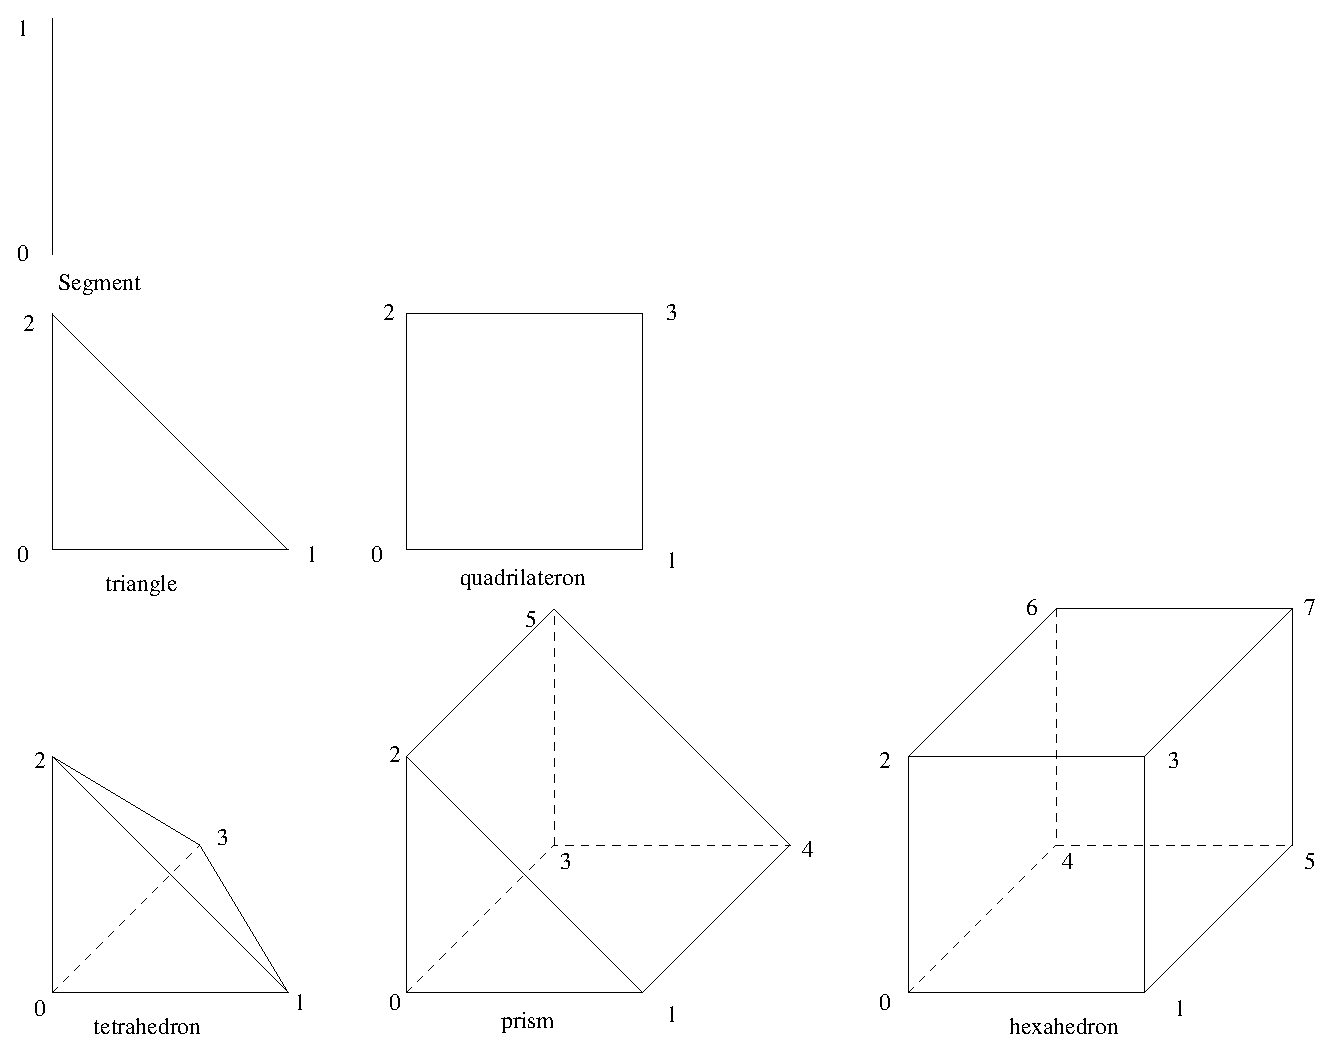
\includegraphics[width=15cm,angle=0]{getfemuserelem}}
    \htmlonly{\htmlimg{getfemuserelem.png}{vertex numeration for usual elements}}
  \end{center}
  \caption{ \it vertex numeration for usual elements }
  \label{fig:elem}
\end{figure}

\subsection{Remove an element from a mesh}
To remove an element from a mesh, simply use\\[0.5cm]
\index{GETFEM!mymesh.sup\_convex(i)}
\cpp{mymesh.sup\_convex(i); }\\[0.5cm]
where \cpp{i} is the index of the element.

\subsection{Simple structured meshes}

For parallelepiped domains, it is possible to obtain structured meshes with simplices, parallelepipeds or prisms elements from three functions defined in \getfemregularmeshesh. \\[0.5cm]

The simplest function is to use 
\begin{cppcode}
  void regular_unit_mesh(mesh& m, std::vector<size_type> nsubdiv, 
                       bgeot::pgeometric_trans pgt, bool noised = false);
\end{cppcode}
which fills the mesh \cpp{m} with a regular mesh of simplices/parallelepipeds/prisms (depending on the value of \cpp{pgt}). The number of cells in each direction if given by \cpp{nsubdiv}. The following example builds a mesh of quadratic triangles on the unit square (the mesh can be scaled and translated afterwards)
\begin{cppcode}
  std::vector<getfem::size_type> nsubdiv(2);
  nsubdiv[0] = 10; nsubdiv[1] = 20;
  regular_unit_mesh(m, nsubdiv, bgeot::simplex_geotrans(2,2));
\end{cppcode}


More specialized regular mesh function are also available:\\


\index{GETFEM!getfem::parallelepiped\_regular\_mesh}
\begin{cppcode}
  getfem::parallelepiped\_regular\_simplex\_mesh(mymesh, N, org, ivect, iref); \\
  getfem::parallelepiped\_regular\_prism\_mesh(mymesh, N, org, ivect, iref); \\
  getfem::parallelepiped\_regular\_mesh(mymesh, N, org, ivect, iref);
\end{cppcode}
where \cpp{mymesh} is a mesh variable in which the structured mesh will be built, \cpp{N} is the dimension (limited to 4 for simplices, 5 for prisms, unlimited for parallelepipeds), \cpp{org} is of type \cpp{bgeot::base\_node} and represents the origin of the mesh, \cpp{ivect} is an iterator on an array of \cpp{N} vectors to build the parallelepiped domain, \cpp{iref} is an iterator on an array of \cpp{N} integers representing the number of division on each direction. \\[0.5cm]
For instance, to build a mesh with tetrahedrons for a unit cube with $10�10�10$ cells one can write\\[0.5cm]
\begin{cppcode}
  getfem::mesh mymesh; \\
  bgeot::base\_node org(0.0, 0.0, 0.0); \\
  std::vector<bgeot::base\_small\_vector> vect(3); \\
  vect[0] = bgeot::base\_small\_vector(1.0, 0.0, 0.0); \\
  vect[1] = bgeot::base\_small\_vector(0.0, 1.0, 0.0); \\
  vect[2] = bgeot::base\_small\_vector(0.0, 0.0, 1.0); \\
  std::vector<int> ref(3); \\
  ref[0] = ref[1] = ref[2] = 10; \\
  getfem::parallelepiped\_regular\_simplex\_mesh(mymesh, 3, org, vect.begin(), ref.begin()); 
\end{cppcode}

Remark: \cpp{base\_node} and \cpp{base\_small\_vector} are almost identical, they are both ``small'' vector classes (they cannot store more than 16 elements), used to describe geometrical points, and geometrical vectors. Their memory footprint is lower than a \cpp{std::vector}.

\subsection{Mesh regions}
A mesh object can contain many \getfemmeshregion objects (declaration in \getfemmeshregionh). These objects are containers for a set of convexes and convex faces. They are used to define boundaries, or a partition of the mesh for parallel solvers, etc.
\begin{cppcode}
  mymesh.region(30).add(3);   // add convex 3 into region 30
  mymesh.region(30).add(4,3); // add face 3 of convex 4 into region 30
  mymesh.sup_convex(4);  // the correspounding entry will be removed from mesh.region(30)
  for (getfem::mr\_visitor i(mymesh.region(30)); !i.finished(); ++i) \{
    cout << "convex: " << i.cv() << " face:" << i.f() << endl;
  \}
\end{cppcode}

\subsection{Methods of the \cpp{getfem::mesh} object}

The list is not exhaustive.

\begin{ctableau}{|m{0.4\linewidth}|m{0.55\linewidth}|}{ll}\hline
  \cpp{mymesh.dim()} & main dimension of the mesh.  \\ \hline
  
  \cpp{mymesh.points\_index()} & gives a \cpp{dal::bit\_vector} object
  which represents all the indexes of valid points of a mesh (see below) \\ \hline
  
  \cpp{mymesh.points()[i]} & gives the point of index \cpp{i} (a
  \cpp{bgeot::base\_node} ). \\ \hline
  
  \cpp{mymesh.convex\_index()} & gives a \cpp{dal::bit\_vector} object
  which represents all the indexes of valid elements of a mesh (see below) \\ \hline
  
  \cpp{mymesh.structure\_of\_convex(i)} & gives the description of the
  structure of element of index \cpp{i}. The function return a
  \bgeotpconvexstructure. \\ \hline
  
  \cpp{mymesh.structure\_of\_convex(i)\hspace{5em}->nb_faces()} & number
  of faces of element of index \cpp{i}. \\ \hline
  
  \cpp{mymesh.structure\_of\_convex(i)\hspace{5em}->nb\_points()} &
  number of vertices of element of index \cpp{i}. \\ \hline
  
  \cpp{mymesh.structure\_of\_convex(i)->dim()} & intrinsic dimension of
  element of index \cpp{i}. \\ \hline
  

  \cpp{mymesh.structure\_of\_convex(i)\hspace{5em}->nb\_points\_of\_face(f)}
  & number of vertices of the face of local index \cpp{f} of element
  of index \cpp{i}.\\ \hline
 

  \cpp{mymesh.structure\_of\_convex(i)\hspace{5em}->ind\_points\_of\_face(f)}
  & return a container with the local indexes of all vertices of the
  face of local index \cpp{f} of element of index \cpp{i}. For
  instance \cpp{mesh.structure\_of\_convex(i)
    ->ind\_points\_of\_face(f)[0]} is the local index of the first
  vertex. \\ \hline
  
  \cpp{mymesh.structure\_of\_convex(i)\hspace{5em}->face\_structure(f)}
  & gives the structure (a \bgeotpconvexstructure) of local
  index \cpp{f} of element of index \cpp{i}.\\ \hline
  
  \cpp{mymesh.ind\_points\_of\_convex(i)} & gives a container with the
  global indexes of vertices of element of index \cpp{i}.\\ \hline
  
  \cpp{mymesh.points\_of\_convex(i)} & gives a container with the
  vertices of element of index \cpp{i}. This is an array of
  \cpp{bgeot::base\_node}.\\ \hline
  
  \cpp{mymesh.convex\_to\_point(ipt)} & gives a container with the
  indexes of all elements attached to the point of global index
  \cpp{ipt}.\\ \hline
  
  \cpp{mymesh.neighbours\_of\_convex(ic, f)} & gives a container with
  the indexes of all elements in \cpp{mesh} having the common face of
  local index \cpp{f} of element \cpp{ic} except element \cpp{ic}. \\ 
  \hline

  \cpp{mymesh.neighbour\_of\_convex(ic, f)} & gives the index of the
  first elements in \cpp{mesh} having the common face of
  local index \cpp{f} of element \cpp{ic} except element \cpp{ic}.
  return size_type(-1) if none is found. \\ 
  \hline

  \cpp{mymesh.is\_convex\_having\_neighbour(ic, f)} & return whether or not
  the element \cpp{ic} has a neighbour with respect to its face of
  local index \cpp{f}. \\ 
  \hline
  
  \cpp{mymesh.clear()} & delete all elements and points from the mesh.
  \\ \hline

  \cpp{mymesh.optimize\_structure()} & compact the structure (renumbers points and convexes such that there is no hole in their numbering). \\ \hline
  
  \cpp{mymesh.trans\_of\_convex(i)} & return the geometric transformation of the
  element of index \cpp{i} (in a \bgeotpgeometrictrans).
  See \cite{BASCOMP} for more details about geometric transformations.  \\ \hline
  
  \cpp{mymesh.normal\_of\_face\_of\_convex(ic, f, pt)} & gives a
  \cpp{bgeot::base\_small\_vector} representing an outward normal to
  the element at the face of local index \cpp{f} at the point of local
  coordinates (coordinates in the element of reference) \cpp{pt}. The
  point \cpp{pt} has no influence if the geometric transformation is
  linear. This is not a unit normal, the norm of the resulting vector
  is the ratio between the surface of the face of the reference
  element and the the surface of the face of the real element. \\ 
  \hline
  
  \cpp{mymesh.convex\_area\_estimate(ic)} & gives an estimate
  of the area of convex \cpp{ic}. \\ \hline

  \cpp{mymesh.convex\_quality\_estimate(ic)} & gives an rought estimate
  of the quality of element \cpp{ic}. \\ \hline
  
  \cpp{mymesh.convex\_radius\_estimate(ic)} & gives an estimate of the
  radius of element \cpp{ic}. \\ \hline 
  
  \cpp{mymesh.region(irg)} & return a \getfemmeshregion. 
  The region is stored in the mesh, and can contain a set of convex
  numbers and or convex faces. \\ \hline

  \cpp{mymesh.has\_region(irg)} & returns true if the region of index \cpp{irg} has been created.\\ \hline
\end{ctableau}

The methods of the convexes/convex faces container \cpp{getfem::mesh\_region} are:
\begin{ctableau}{|m{0.4\linewidth}|m{0.55\linewidth}|}{ll}\hline
  \cpp{add(ic)} & add the convex of index \cpp{ic} to the region\\ \hline
  \cpp{add(ic,f)} & add the face number \cpp{f} of the convex \cpp{ic}\\ \hline
  \cpp{sup(ic)}, \cpp{sup(ic,f)} & remove the convex or the convex face from the region\\ \hline
  \cpp{is\_in(ic)}, \cpp{is\_in(ic,f)} & return true if the convex (or convex face) is in the region.\\ \hline
  \cpp{is\_only\_faces()} & return true if the region does not contain any convex.\\ \hline
  \cpp{is\_only\_convexes()} & return true if the region does not contain any convex face.\\ \hline
  \cpp{index()} & return a \cpp{dal::bit\_vector} containing the list of convexes which are stored (or whose faces are stored) in the region.\\\hline
\end{ctableau}

Iteration over a \getfemmeshregion should be done with \getfemmrvisitor:
\begin{cppcode}
  getfem::mesh\_region &rg = mymesh.region(2);
  for (getfem::mr\_visitor i(rg); !i.finished(); ++i) \{
    cout << "contains convex " < < i.cv();
    if (i.is\_face()) cout  << "face " << i.f() << endl;
  \}
\end{cppcode}

\subsection{Using dal::bit_vector}
The object \dalbitvector (declared in \dalbitvectorh) is a structure heavily used in \gf.
It is very close to \cpp{std::bitset} and \cpp{std::vector<bool>} but
with additional functionalities to represent a set of non negative
integers and iterate other them. 

If \cpp{nn} is declared to be a \cpp{dal::bit\_vector}, the
two instructions \cpp{nn.add(6)} or \cpp{nn[6] = true} are equivalent
and means that integer 6 is added to the set. 

In a same way \cpp{nn.sup(6)} or \cpp{nn[6] = false} remove the integer 6 from the
set. The instruction \cpp{nn.add(6, 4)} adds 6,7,8,9 to the set.

To iterate on a
\cpp{dal::bit\_vector}, it is possible to use iterators as usual, but,
most of the time, as this object represents a set of integer, one just
wants to iterate on the integers included into the set. The simplest
way to do that is to use the pseudo-iterator \dalbvvisitor.

For instance, here is the code to iterate on
the points of a mesh and print it to the standard output
\begin{cppcode}
  for (dal::bv\_visitor i(mymesh.points\_index()); !i.finished(); ++i)
    cout << "Point of index " << i << " of the mesh : " << mymesh.points()[i] << endl;
\end{cppcode}

\subsection{Face numbering}
The numeration of faces on usual elements is given in figure~\ref{fig:elemf}.
\begin{figure}[htb]
  \begin{center}
    \texonly{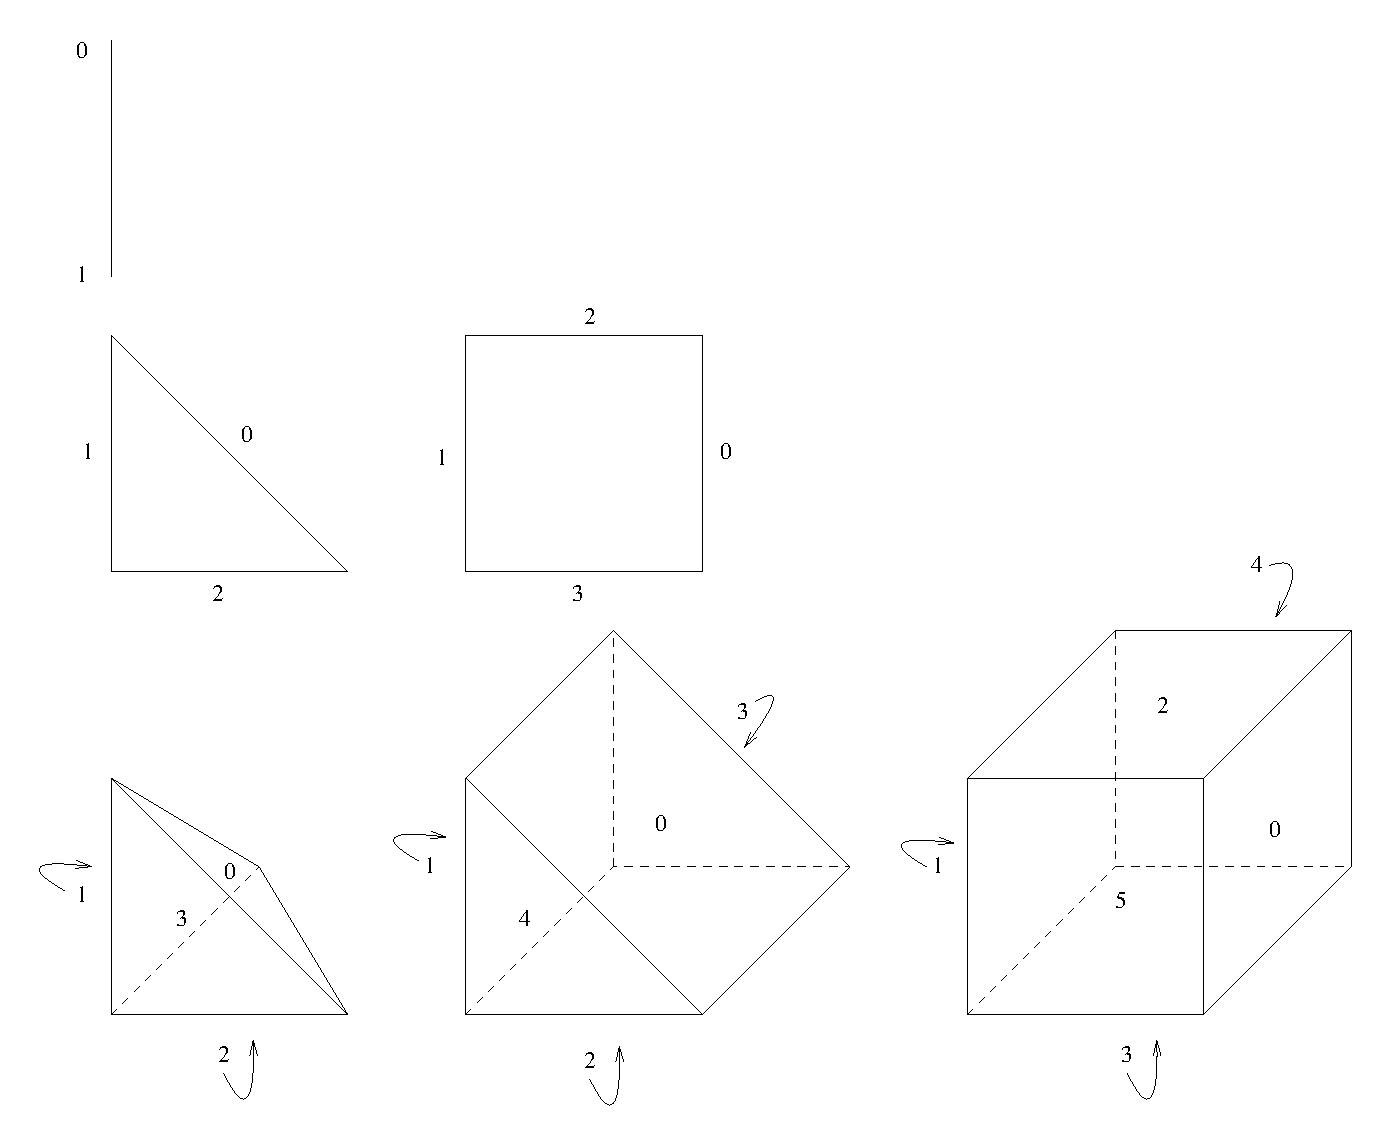
\includegraphics[width=15cm,angle=0]{getfemuserelemf}}
    \htmlonly{\htmlimg{getfemuserelemf.png}{faces numeration for usual elements}}
  \end{center}
  \caption{ \it faces numeration for usual elements }
  \label{fig:elemf}
\end{figure}

Note that, while the convexes and the points are globaly numbered in a \cpp{getfem::mesh} object, there is no global numbering of the faces, so the only way to refer to a given face, is to give the convex number, and the local face number in the convex.

\subsection{Save and load meshes}

\subsubsection{ From getfem file format}

In \getfemmeshh, two methods are defined to load meshes from file and write meshes to a file. \\[0.5cm]
\index{GETFEM!mymesh.write\_to\_file(name)}
\index{GETFEM!mymesh.read\_from\_file(name)}
\begin{ctableau}{|m{0.4\linewidth}|m{0.55\linewidth}|}{ll}\hline

  \cpp{mymesh.write\_to\_file(const std::string \&name)} & save the mesh into a file.\\ \hline

  \cpp{mymesh.read\_from\_file(const std::string \&name)} & load the mesh from a file.\\ \hline
\end{ctableau}


The following is an example of how to load a mesh and extract information on it.
\begin{cppcode}
  \#include <getfem/getfem\_mesh.h>
  
  getfem::mesh mymesh; 
  
  int main(int argc, char *argv[]) \{ 
    try \{ 
     
      // read the mesh from the file name given by the first argument 
      mymesh.read\_from\_file(std::string(argv[1])); 
     
      // List all the convexes
      dal::bit\_vector nn = mymesh.convex\_index(); 
      bgeot::size\_type i; 
      for (i << nn; i != bgeot::size\_type(-1); i << nn) \{
        cout << "Convex of index " << i << endl; 
        bgeot::pconvex\_structure cvs =  mymesh.structure\_of\_convex(i); 
        cout << "Number of vertices : " << cvs->nb\_points() << endl; 
        cout << "Number of faces : " << cvs->nb\_faces() << endl;
        for (bgeot::size\_type f = 0; f < cvs->nb\_faces(); ++f) \{
          cout << "face " << f << " has " << cvs->nb\_points\_of\_face(f); 
          cout << " vertices with local indexes : "; 
          for (bgeot::size\_type k = 0; k < cvs->nb\_points\_of\_face(f); ++k) 
          cout << cvs->ind\_points\_of\_face(f)[k] << " "; 
          cout << " and global indexes : ";
          for (bgeot::size\_type k = 0; k < cvs->nb\_points\_of\_face(f); ++k) 
            cout << mymesh.ind\_points\_of\_convex(i)[cvs->ind\_points\_of\_face(f)[k]] << " ";
        \}
     \}
     
   \} GMM\_STANDARD\_CATCH\_ERROR; // catches standard errors
 \}
\end{cppcode}

\subsubsection{Import a mesh}

The file \getfemimporth provides the function:
\begin{cppcode}
  void import_mesh(const std::string\& fmtfilename, mesh\& m);
\end{cppcode}
Here the string \cpp{fmtfilename} must contain a descriptor of the file format ("gid", "gmsh", "am_fmt", "emc2_mesh", or "structured") , followed by a colon and the file name (if there is not format descriptor, it is assumed that the file is a native getfem mesh and the \cpp{mesh::read_from_file()} method is used).

Example:
\begin{cppcode}
getfem::mesh m;
getfem::import_mesh("gid:../tests/meshes/tripod.GiD.msh",m);
\end{cppcode}

The "gid" format is for meshes generated by \WEB{http://gid.cimne.upc.es/}{GiD}. The "gmsh" is for meshes generated by the open-source mesh generator \WEB{http://www.geuz.org/gmsh/}{GMSH}, and the "am_fmt" and "emc2_mesh" are for files built with \WEB{http://www-rocq1.inria.fr/gamma/cdrom/www/emc2/eng.htm}{emc2} (free but 2D only)

The "structured" format is just a short specification for regular meshes: the rest of \cpp{fmtfilename} in that case is not a filename, but a string whos format is following:
\begin{cppcode}
getfem::import_mesh("structured:GT='GT_PK(2,1)'; NSUBDIV=[5,5]; ORG=[0,0]; SIZES=[1,1]; NOISED=0", m);
\end{cppcode}
where GT is the name of the geometric transformation, NSUBDIV a vector of the number of subdivisions in each coordinate (default value 2), ORG is the origin of the mesh (default value [0,0,...]), SIZES is a vector of the sizes
in each direction (default value [1, 1, ...] and if NOISED=1 the nodes
of the interior of the mesh are randomly "shaken"(default value NOISED=0).
In that string, all the parameters are optional except GT.



\section{Build a finite element method on a mesh}
The object \getfemmeshfem defined in \getfemmeshfemh is desined to describe a finite element method on a whole mesh, i.e. to describe the finite element space on which some variables will be describe. This is a rather complex object which is central in \gf. Basically, this structure describes the finite element method on each element of the mesh and some additional optional transformations. It is possible to have an arbitrary number of finite element description for a single mesh. This is particularly necessary for mixed methods, but also to describe different data on the same mesh. One can instantiate a \cpp{getfem::mesh\_fem} object as follows
\begin{cppcode}
  getfem::mesh\_fem mf(mymesh);
\end{cppcode}
where \cpp{mymesh} is an already existing mesh. The structure will be linked to this mesh and will react when modifications will be done on it. \\[0.5cm]
It is possible to specify element by element the finite element method, so that element of mixed types can be treated, even if the dimensions are different. For usual elements, the connection between two elements is done when the two elements are compatibles (same degrees of freedom on the common face). A numeration of the degrees of freedom is automatically done with a Cuthill Mc Kee like algorithm. You have to keep in mind that there is absolutely no connection between the numeration of vertices of the mesh and the numeration of the degrees of freedom. Every \cpp{getfem::mesh\_fem} object has its own numeration. \\[0.5cm]

There is three levels in the \getfemmeshfem object:
\begin{itemize}
  \item The element level : one finite element method per element. It is possible to mix the dimensions of the elements and the property to be vectorial or scalar.
  \item The optional vectorization (the qdim in getfem jargon, see \WEB{http://download.gna.org/getfem/doc/getfem_project/getfem_project_4.html}). For instance to represent a deplacement fiels in continuum mechanics. Scalar elements are used componentwise. Note that you can mix some intrinsic vectorial elements (Raviart-Thomas element for instance) which will not be vectorized and some scalar element which will be.
\item (\gf version 4.0) The optional additional linear transformation (reduction) of the degrees of freedom. It will consist in giving two matrices, the reduction matrix and the extension matrix. The reduction matrix should transform the basic dofs into the reduced dofs (the number of reduced dofs should be less or equal than the number of basic dofs). The extension matrix should describe the inverse transformation. The product of the reduction matrix with the extension matrix should be the identity matrix (ensuring in particular that the two matrices are of maximal rank). This optional transformation can be used to reduced the finite element space to a certain region (tipically a boundary) or to prescribe some matching conditions between non naturally compatible fems (for instance fems with different degrees).
\end{itemize}

One has to keep in mind this construction manipulating the degrees of freedom of a \getfemmeshfem object.

\subsection{first level : manipulating fems on each elements}

To select a particular finite element method on a given element, use the method
\index{GETFEM!mf.set\_finite\_element(i, pf)}
\begin{cppcode}
  mf.set\_finite\_element(i, pf);
\end{cppcode}
where \cpp{i} is the index of the element and \cpp{pf} is the descriptor (of type \getfempfem, basically a pointer to an object which inherits from \getfemvirtualfem) of the finite element method. Alternative forms of this member function are:
\begin{cppcode}
  void mesh\_fem::set\_finite\_element(const dal::bit\_vector &cvs, 
                                    getfem::pfem pf);
  void mesh\_fem::set\_finite\_element(getfem::pfem pf);
\end{cppcode}
which set the finite elements for either the convexes listed in the \cpp{bit\_vector cvs}, or all the convexes of the mesh. Note that the last method make an call to the method
\begin{cppcode}
  void mesh\_fem::set_auto_add(pfem pf);
\end{cppcode}
which defines the default finite element method which will be automatically added on new elements of the mesh (this is very usefull, for instance, when a refinement of the mesh is performed).

Descriptors for finite element methods and integration methods are available thanks to the following function\\[0.5cm]
\index{GETFEM!getfem::fem\_descriptor("name")}\index{GETFEM!getfem::pfem}
\begin{cppcode}
  getfem::pfem pf = getfem::fem\_descriptor("name of method");
\end{cppcode}
where \cpp{"name of method"} is to be chosen among the existing methods.
A name of a method can be retrieved thanks to the following functions\\[0.5cm]
\begin{cppcode}
  std::string femname = getfem::name\_of\_fem(pf);
\end{cppcode}
A non exhautive list (see Appendix A or \getfemfemh for exhaustive lists) of finite element methods is given by

\begin{center} \begin{tabular}{|m{0.40\linewidth}|m{0.55\linewidth}|} \hline
{\tt "FEM\_PK(n,k)"} & Classical $P_K$ methods on simplexes of dimension  {\tt n} with degree {\tt k} polynomials.\\ \hline
\end{tabular}  
\begin{tabular}{|m{0.40\linewidth}|m{0.55\linewidth}|} \hline
{\tt "FEM\_QK(n,k)"} & Classical $Q_K$ methods on parallelepiped of dimension {\tt n}. Tensorial product of degree {\tt k} $P_K$ method on the segment. \\ \hline
\end{tabular}  
\begin{tabular}{|m{0.40\linewidth}|m{0.55\linewidth}|} \hline
{\tt "FEM\_PK\_PRISM(n,k)"} & Classical methods on prism of dimension {\tt n}. Tensorial product of two degree {\tt k} $P_K$ method. \\ \hline
\end{tabular}  
\begin{tabular}{|m{0.40\linewidth}|m{0.55\linewidth}|} \hline
{\tt "FEM\_PRODUCT(a,b)"} & Tensorial product of the two polynomial finite element method {\tt a} and {\tt b}. \\ \hline
\end{tabular}   
\begin{tabular}{|m{0.40\linewidth}|m{0.55\linewidth}|} \hline
{\tt "FEM\_PK\_DISCONTINUOUS(n,k)"} & discontinuous $P_K$ methods on simplexes of dimension  {\tt n} with degree {\tt k} polynomials. \\ \hline
\end{tabular}  
\end{center}

An alternative way to obtain a Lagrange polynomial fem suitable for a given geometric transformation is to use
\index{GETFEM!getfem::classical\_fem(pgt,degree)}\index{GETFEM!getfem::classical\_discontinuous\_fem(pgt,degree)}
\begin{cppcode}
 getfem::pfem getfem::classical\_fem(bgeot::pgeometric\_trans pg, short\_type degree);
 pfem getfem::classical\_discontinuous\_fem(bgeot::pgeometric\_trans pg, short\_type degree);
\end{cppcode}

The \cpp{mesh\_fem} can call directly these functions via:\index{GETFEM!getfem::set_classical\_finite\_element}\index{GETFEM!getfem::set\_classical\_discontinuous\_finite\_element}
\begin{cppcode}
  void mesh\_fem::set\_classical\_finite\_element(const dal::bit\_vector &cvs, 
                                              dim\_type fem\_degree);
  void mesh\_fem::set\_classical\_discontinuous\_finite\_element
         (const dal::bit\_vector &cvs, dim\_type fem\_degree);
  void mesh\_fem::set\_classical\_finite\_element(dim\_type fem\_degree);
  void mesh\_fem::set\_classical\_discontinuous\_finite\_element(dim\_type fem\_degree);                           
\end{cppcode}

Some other methods: \\[0.5cm]
\begin{center} \texonly{\begin{tabular}{|m{0.4\linewidth}|m{0.55\linewidth}|} \hline}\htmlonly{\xmlattributes*{table}{border}\begin{tabular}{l|l}}

  \cpp{mf.convex\_index()} & Set of indexes (a \cpp{dal::bit\_vector}) on which a finite element method is defined.  \\ \hline

  \cpp{mf.linked\_mesh()} & gives a reference to the linked mesh.  \\ \hline

  \cpp{mf.fem\_of\_element(i)} & gives a descriptor on the finite element method defined on element of index \cpp{i} (does not take into account the qdim nor the optional reduction).  \\ \hline

  \cpp{mf.clear()} & Clear the structure, no finite element method is still defined.  \\ \hline
\end{tabular} \end{center}

\subsection{Examples}
For instance if one needs to have a description of a $P_1$ finite element method on a triangle, the way to set it is
\begin{cppcode}
 mf.set\_finite\_element(i, getfem::fem\_descriptor("FEM\_PK(2, 1)"));
\end{cppcode}
where \cpp{i} is still the index of the triangle. It is also possible to select a particular method directly on a set of element, passing to \cpp{mf.set\_finite\_element} a \cpp{dal::bit\_vector} instead of a single index. For instance
\begin{cppcode}
 mf.set\_finite\_element(mymesh.convex\_index(), 
                         getfem::fem\_descriptor("FEM\_PK(2, 1)"));
\end{cppcode}
selects the method on all the elements of the mesh.\\[0.5cm]

\subsection{Second level : the optional ``vectorization''}

If the finite element represents an unknown for a vectorial
problem, one should
use \cpp{mf.set\_qdim(Q)} to set the target dimension for the definition of the target dimension $Q$).\\[0.5cm]
If the target dimension $Q$ is set to a value different of $1$, the
scalar FEMs (such as $P_k$ fems etc.) are automatically
``vectorized'', i.e. each scalar degree of freedom is duplicated $Q$
times, from the \cpp{mesh\_fem} object point of vue. To sum it up,
\begin{itemize}
\item if the fem of the $ith$ element is intrinsically a vector FEM,\\
 \cpp{mf.get\_qdim() == mf.fem\_of\_element(i)->target\_dim()} 
\\ and\\ \cpp{mf.nb\_dof\_of\_element(i) == mf.fem\_of\_element(i).nb\_dof()}.
\item if the fem has a \cpp{target\_dim} equal to $1$, \\
\cpp{mf.nb\_dof\_of\_element(i) == mf.get\_qdim()*mf.fem\_of\_element(i).nb\_dof()}.
\end{itemize}

At this level are defined the basic degrees of freedom. Some methods of the \getfemmeshfem allows to obtain information on the basic dofs:\\[0.5cm]
\begin{center} \texonly{\begin{tabular}{|m{0.4\linewidth}|m{0.55\linewidth}|} \hline}\htmlonly{\xmlattributes*{table}{border}\begin{tabular}{l|l}}

  \cpp{mf.nb\_basic\_dof\_of\_element(i)} & gives the number of basic degrees of freedom on the element of index \cpp{i}.  \\ \hline

  \cpp{mf.ind\_basic\_dof\_of\_element(i)} & gives a container (an array) with all the global indexes of the basic degrees of freedom of element of index \cpp{i}.  \\ \hline

  \cpp{mf.point\_of\_basic\_dof(i, j)} & gives a \cpp{bgeot::base\_node} which represents the point associated with the basic dof of local index \cpp{j} on element of index \cpp{i}.  \\ \hline

  \cpp{mf.point\_of\_basic\_dof(j)} & gives a \cpp{bgeot::base\_node} which represents the point associated with the basic dof of global index \cpp{j}.  \\ \hline

  \cpp{mf.reference\_point\_of\_basic\_dof(i, j)} & gives a \cpp{bgeot::base\_node} which represents the point associated with the basic dof of local index \cpp{j} on element of index \cpp{i} in the coordinates of the reference element.  \\ \hline

  \cpp{mf.first\_convex\_of\_basic\_dof(j)} & gives the index of the first element on which the basic degree of freedom of global index \cpp{j} is defined.  \\ \hline
  
  \cpp{mf.nb\_basic\_dof()} & gives the total number of different basic degrees of freedom.  \\ \hline

  \cpp{mf.get_qdim()} & gives the target dimension \cpp{Q}.  \\ \hline

  \cpp{mf.basic\_dof\_on\_region(i)} & Return a \cpp{dal::bit_vector} which represent the indices of basic dof which are in the set of convexes or the set of faces of index \cpp{i} (see the \cpp{getfem::mesh} object).  \\ \hline

  \cpp{mf.dof\_on\_region(i)} & Return a \cpp{dal::bit_vector} which
  represent the indices of dof which are in the set of convexes or the
  set of faces of index \cpp{i} (see the \cpp{getfem::mesh} object).
  For a reduced mesh_fem,
  a dof is lying on a region if its potential corresponding shape
  function is nonzero on this region. The extension matrix is used
  to make the correspondance between basic and reduced dofs. \\ \hline
\end{tabular} \end{center}


\subsection{Third level : the optional linear transformation (or reduction)}

As describe above, it is possible to provide two matrices, a reduction matrix $R$ and an extension matrix $E$ which will describe a linear transforamtion of the degrees of freedom. If $V$ is the vector of basic degrees of freedom, then $U=RV$ will be the vector of reduced degrees of freedom. Contrarily, given a vector $U$ of reduced dof, $V=EU$ will correspond to a vector of basic dof. In simle cases, $E$ will be simply the transpose of $R$. NOTE that every line of the extension matrix should be sparse. Otherwise, each assembled matrix will be plain !

A natural condition is that $RE = I$ where $I$ is the identity matrix.


\begin{center} \texonly{\begin{tabular}{|m{0.4\linewidth}|m{0.55\linewidth}|} \hline}\htmlonly{\xmlattributes*{table}{border}\begin{tabular}{l|l}}

  \cpp{mf.nb\_dof()} & gives the total number of different degrees of freedom. If the optional reduction is used, this will be the number of columns of the reduction matrix. Otherwise it will return the number of basic degrees of freedom.  \\ \hline

  \cpp{mf.is\_reduced()} & return a boolean. True if the reduction is used.  \\ \hline

  \cpp{mf.reduction\_matrix()} &  return a const reference to the reduction matrix $R$. \\ \hline

  \cpp{mf.extension\_matrix()} &  return a const reference to the extension matrix $E$. \\ \hline

  \cpp{mf.set\_reduction\_matrices(R, E)} &  Set the reduction and extension matrices to \cpp{R} and \cpp{E} and valid their use. \\ \hline

  \cpp{mf.set\_reduction(b)} &  Where $b$ is a boolean. Cancel the reduction if $b$ is true and valid it is \cpp{b} is true. If \cpp{b} is true, the extension and reduction matrices have to be set previously.\\ \hline

  \cpp{mf.reduce_to_basic_dof(idof)} & Set the reduction and extension matricescorrespondinf to keep only the basic dofs present in \cpp{idof}. The parameter \cpp{idof} is either a \cpp{dal::bit_vector} or a \cpp{std::set<size\_type>}. This is equivalent to the use of a \cpp{getfem::partial\_mesh\_fem} object.\\ \hline

\end{tabular} \end{center}

\subsection{Obtaining generic mesh\_fems}

It is possible to use the function
\begin{cppcode}
  const mesh_fem &getfem::classical_mesh_fem(const getfem::mesh &mymesh, dim_type K);  
\end{cppcode}
to get a classical polynomial \cpp{mesh_fem} of order $K$ on the given
\cpp{mymesh}.  The returned mesh\_fem will be destroyed automatically
when its linked_mesh is destroyed. All the \cpp{mesh_fem} built by
this function are stored in a cache, which means that calling this
function twice with the same arguments will return the same
\cpp{mesh_fem} object. A consequence is that you should NEVER modify
this mesh\_fem!

\subsection{The  partial\_mesh\_fem object}
\index{GETFEM!getfem::partial\_mesh\_fem}

The \cpp{getfem::partial\_mesh\_fem} object defined in the file \cpp{getfem_partial\_mesh\_fem.h} allows to reduce a \cpp{getfem::mesh\_fem} object to a set of dofs. The interest is this is not a complete description of a finite element method, it refers to the original \cpp{getfem::mesh\_fem} and just add reduction and extension matrices. For instance, you can reduce a \cpp{mesh\_fem} obtained by the function \cpp{getfem::classical\_mesh\_fem(mesh, K)} to obtain a finite element method on a mesh region (which can be a boundary). The \cpp{getfem::partial\_mesh\_fem} is in particular used to obtain multiplier description to prescribed boundary conditions. 

The declaration of a \cpp{getfem::partial\_mesh\_fem} object is the following:
\begin{cppcode}
  getfem::partial\_mesh\_fem(mf) partial\_mf;
\end{cppcode}

Then, one has to call the adapt method as follows:
\begin{cppcode}
  partial\_mf.adapt(kept\_dof, rejected\_elt = dal::bit\_vector());
\end{cppcode}
where \cpp{kept\_dof} and \cpp{rejected\_elt} are some \cpp{dal::bit\_vector()}. \cpp{kept\_dof} is the list of dof indices of the original \cpp{mesh\_fem} \cpp{mf} to be kept. \cpp{rejected\_elt} is an optional parameter that contains a list of element indices on which the \cpp{getfem::partial\_mesh\_fem} states that there is no finite element method. This is to avoid unnecessary computations during assembly procedures.

\section{Selecting integration methods}
\index{GETFEM!getfem::mesh\_im}

The description of an integration method on a whole mesh is done
thanks to the structure \cpp{getfem::mesh\_im}, defined in the file
\getfemmeshimh. Basically, this structure describes the integration
method on each element of the mesh. One can instantiate a
\cpp{getfem::mesh\_im} object as follows\\[0.5cm]

\begin{cppcode}
 getfem::mesh\_im mim(mymesh);
\end{cppcode}

where \cpp{mymesh} is an already existing mesh. The structure will be
linked to this mesh and will react when modifications will be done on
it (for example when the mesh is refined, the integration method will
be also refined).\\[0.5cm]

It is possible to specify element by element the integration method,
so that element of mixed types can be treated, even if the dimensions
are different.\\[0.5cm]

To select a particular integration method on a given element, one can
use\\[0.5cm]
\index{GETFEM!mim.set\_integration\_method(i, ppi)}
\cpp{mf.set\_integration\_method(i, ppi); }\\[0.5cm]
where \cpp{i} is the index of the element and \cpp{ppi} is the
descriptor of the integration method. Alternative forms of this member
function are:
\begin{cppcode}
  void mesh\_fem::set\_integration\_method(const dal::bit\_vector &cvs, 
    getfem::pintegration\_method ppi);
  void mesh\_fem::set\_integration\_method(getfem::pintegration\_method ppi);
\end{cppcode}
which set the integration method for either the convexes listed in the \cpp{bit\_vector} cvs, or all the convexes of the mesh.

The list of all available descriptors of integration methods is in the file \getfemintegrationh. \\[0.5cm]
Descriptors for integration methods are available thanks to the following function:
\index{GETFEM!getfem::int\_method\_descriptor("name")}\index{GETFEM!getfem::pintegration_method}
\begin{cppcode}
  getfem::pintegration_method ppi = 
            getfem::int\_method\_descriptor("name of method");
\end{cppcode}
where \cpp{"name of method"} is to be chosen among the existing methods.
A name of a method can be retrieved with
\begin{cppcode}
  std::string im\_name = getfem::name\_of\_int\_method(ppi);
\end{cppcode}
A non exhautive list (see Appendix B or \getfemintegrationh for exhaustive lists) of integration methods is given below.

Examples of exact integration methods:
\begin{center} \begin{tabular}{|m{0.4\linewidth}|m{0.55\linewidth}|} \hline
{\tt "IM\_NONE()"} & Dummy integration method (new in getfem++-1.7).\\ \hline
\end{tabular}  
\begin{tabular}{|m{0.4\linewidth}|m{0.55\linewidth}|} \hline
{\tt "IM\_EXACT\_SIMPLEX(n)"} & Description of the exact integration of polynomials on the simplex of reference of dimension {\tt n}. \\ \hline
\end{tabular}  
\begin{tabular}{|m{0.4\linewidth}|m{0.55\linewidth}|} \hline
{\tt "IM\_PRODUCT(a, b)"} & Description of the exact integration on the convex which is the direct product of the convex in {\tt a} and in {\tt b}.\\ \hline
\end{tabular}  
\begin{tabular}{|m{0.4\linewidth}|m{0.55\linewidth}|} \hline
{\tt "IM\_EXACT\_PARALLELEPIPED(n)"} & Description of the exact integration of polynomials on the parallelepiped of reference of dimension {\tt n}\\ \hline
\end{tabular}  
\begin{tabular}{|m{0.4\linewidth}|m{0.55\linewidth}|} \hline
{\tt "IM\_EXACT\_PRISM(n)"} & Description of the exact integration of polynomials on the prism of reference of dimension {\tt n}\\ \hline
\end{tabular} \end{center}
Examples of approximated integration methods:
\begin{center} \begin{tabular}{|m{0.55\linewidth}|m{0.4\linewidth}|} \hline
{\tt "IM\_GAUSS1D(k)" } & Description of the Gauss integration on a segment of order {\tt k}. \\ \hline
\end{tabular}  
\begin{tabular}{|m{0.55\linewidth}|m{0.4\linewidth}|} \hline
{\tt "IM\_NC(n,k)"} & Description of the integration on a simplex of reference of dimension {\tt n} for polynomials of degree {\tt k} with the Newton Cotes method (based on Lagrange interpolation).\\ \hline
\end{tabular}  
\begin{tabular}{|m{0.55\linewidth}|m{0.4\linewidth}|} \hline
{\tt "IM\_PRODUCT(a,b)"} & Build a method doing the direct product of methods {\tt a} and {\tt b}. \\ \hline
\end{tabular}  
\begin{tabular}{|m{0.55\linewidth}|m{0.4\linewidth}|} \hline
{\tt "IM\_TRIANGLE(2)"} & Integration on a triangle of order 2 with 3 points. \\ \hline
\end{tabular}
\begin{tabular}{|m{0.55\linewidth}|m{0.4\linewidth}|} \hline
{\tt "IM\_TRIANGLE(7)"} & Integration on a triangle of order 7 with 13 points. \\ \hline
\end{tabular} 
\begin{tabular}{|m{0.55\linewidth}|m{0.4\linewidth}|} \hline
{\tt "IM\_QUAD(2)"} & Integration on quadrilaterals of order 2 with 3 points. \\ \hline
\end{tabular}
\begin{tabular}{|m{0.55\linewidth}|m{0.4\linewidth}|} \hline
{\tt "IM\_TETRAHEDRON(5)"} & Integration on a tetrahedron of order 5 with 15 points. \\ \hline
\end{tabular} \end{center}

%\begin{center} \begin{tabular}{|m{0.4\linewidth}|m{0.55\linewidth}|} \hline
%{\tt "IM\_GAUSS1D(k)" } & Description of the Gauss integration on a segment of order {\tt k}. Available for all odd values of k <= 99.\\ \hline
%\end{tabular}  
%\begin{tabular}{|m{0.4\linewidth}|m{0.55\linewidth}|} \hline
%{\tt "IM\_NC(n,k)"} & Description of the integration on a simplex of reference of dimension {\tt n} for polynomials of degree {\tt k} with the Newton Cotes method (based on Lagrange interpolation).\\ \hline
%\end{tabular}  
%\begin{tabular}{|m{0.4\linewidth}|m{0.55\linewidth}|} \hline
%{\tt "IM\_PRODUCT(a,b)"} & Build a method doing the direct product of methods {\tt a} and {\tt b}. \\ \hline
%\end{tabular}  
%\begin{tabular}{|m{0.4\linewidth}|m{0.55\linewidth}|} \hline
%{\tt "IM\_TRIANGLE(2)"} & Integration on a triangle of order 2 with 3 points. \\ \hline
%\end{tabular}
%\begin{tabular}{|m{0.4\linewidth}|m{0.55\linewidth}|} \hline
%{\tt "IM\_TRIANGLE(7)"} & Integration on a triangle of order 7 with 13 points. \\ \hline
%\end{tabular} 
%\begin{tabular}{|m{0.4\linewidth}|m{0.55\linewidth}|} \hline
%{\tt "IM\_TRIANGLE(19)"} & Integration on a triangle of order 19 with 73 points. \\ \hline
%\end{tabular} 
%\begin{tabular}{|m{0.4\linewidth}|m{0.55\linewidth}|} \hline
%{\tt "IM\_QUAD(2)"} & Integration on quadrilaterals of order 2 with 3 points. \\ \hline
%\end{tabular}
%\begin{tabular}{|m{0.4\linewidth}|m{0.55\linewidth}|} \hline
%{\tt "IM\_GAUSS\_PARALLELEPIPED(2,3)"} & Integration on quadrilaterals of order 3 with 4 points (shortcut for {\tt "IM\_PRODUCT(IM\_GAUSS1D(3),IM\_GAUSS1D(3))"}). \\ \hline
%\end{tabular}
%\begin{tabular}{|m{0.4\linewidth}|m{0.55\linewidth}|} \hline
%{\tt "IM\_TETRAHEDRON(5)"} & Integration on a tetrahedron of order 5 with 15 points. \\ \hline
%\end{tabular} \end{center}
\begin{center} \begin{tabular}{|m{0.4\linewidth}|m{0.55\linewidth}|} \hline
{\tt "IM\_GAUSS1D(k)" } & Description of the Gauss integration on a segment of order {\tt k}. Available for all odd values of k <= 99.\\ \hline
{\tt "IM\_NC(n,k)"} & Description of the integration on a simplex of reference of dimension {\tt n} for polynomials of degree {\tt k} with the Newton Cotes method (based on Lagrange interpolation).\\ \hline
{\tt "IM\_PRODUCT(a,b)"} & Build a method doing the direct product of methods {\tt a} and {\tt b}. \\ \hline
{\tt "IM\_TRIANGLE(2)"} & Integration on a triangle of order 2 with 3 points. \\ \hline
{\tt "IM\_TRIANGLE(7)"} & Integration on a triangle of order 7 with 13 points. \\ \hline
{\tt "IM\_TRIANGLE(19)"} & Integration on a triangle of order 19 with 73 points. \\ \hline
{\tt "IM\_QUAD(2)"} & Integration on quadrilaterals of order 2 with 3 points. \\ \hline
{\tt "IM\_GAUSS\_PARALLELEPIPED(2,3)"} & Integration on quadrilaterals of order 3 with 4 points (shortcut for {\tt "IM\_PRODUCT(IM\_GAUSS1D(3),IM\_GAUSS1D(3))"}). \\ \hline
{\tt "IM\_TETRAHEDRON(5)"} & Integration on a tetrahedron of order 5 with 15 points. \\ \hline
\end{tabular} \end{center}

Remark: note that \texttt{IM\_QUAD(3)} is not able to integrate
exactly the base functions of the \texttt{FEM_QK(2,3)} finite element!
Since its base function are tensorial product of 1D polynomials of
degree 3, one would need to use \texttt{IM\_QUAD(7)} (6 is not
available). Hence \texttt{IM\_GAUSS\_PARALLELEPIPED(2,k)} should
always be prefered over \texttt{IM\_QUAD(2*k)} since it has less
integration points.

An alternative way to obtain integration methods: \index{GETFEM!getfem::classical\_exact\_im(pgt)}\index{GETFEM!getfem::classical\_approx\_im(pgt,degree)}
\begin{cppcode}
  getfem::pintegration\_method 
    getfem::classical\_exact\_im(bgeot::pgeometric\_trans pgt);
  getfem::pintegration\_method 
    getfem::classical\_approx\_im(bgeot::pgeometric\_trans pgt, dim\_type d);
\end{cppcode}
These functions return an exact (i.e. analytical) integration method, or select an approximate integration method which is able to integrate exactly polynomials of degree <= \cpp{d} (at least) for convexes defined with the specified geometric transformation.

\subsection{Methods of the \cpp{mesh\_im} object}

Once an integration method is defined on a mesh, it is possible to obtain information on it with the following methods (the list is not exhaustive).\\[0.5cm]
\begin{center} \texonly{\begin{tabular}{|m{0.4\linewidth}|m{0.55\linewidth}|} \hline}\htmlonly{\xmlattributes*{table}{border}\begin{tabular}{l|l}}

  \cpp{mim.convex\_index()} & Set of indexes (a \cpp{dal::bit\_vector}) on which an integration method is defined.  \\ \hline

  \cpp{mim.linked\_mesh()} & gives a reference to the linked mesh.  \\ \hline

  \cpp{mim.int\_method\_of\_element(i)} & gives a descriptor on the integration method defined on element of index \cpp{i}.  \\ \hline

  \cpp{mim.clear()} & Clear the structure, no finite element method is still defined.  \\ \hline

\end{tabular} \end{center}


\section{Mesh refinement}

Mesh refinement with the Bank et all method (see \cite{bank1983}) is available in dimension
1, 2 or 3 for simplex meshes (segments, triangles and tetrahedrons).
For a given object \cpp{mymesh} of type \getfemmesh, the method
\begin{cppcode}
  mymesh.Bank_refine(bv);
\end{cppcode}
refines the elements whose indices are stored in \cpp{bv} (a
\dalbitvector object). The conformity of the mesh is kept
thanks to additional refinement (the so called green triangles). Information about green triangles is stored on the mesh object to gather them for further refinements (see \cite{bank1983}).


\begin{figure}[htb]
  \begin{center}
    \texonly{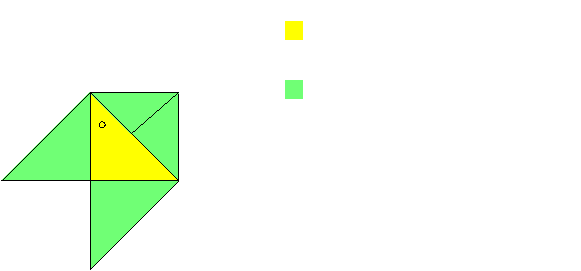
\includegraphics[width=10cm,angle=0]{getfemuserrefine.pdf}}
    \htmlonly{\htmlimg{getfemuserrefine.png}{Example of refinement}}
  \end{center}
  \caption{ \it Exemple of Bank refinement in 2D.}
  \label{fig:refine}
\end{figure}


Mesh refinement is most of the time coupled with an {\it a posteriori} error estimate. A basic error estimate is available in the file \getfemerrorestimateh. 
\begin{cppcode}
  error_estimate(mim, mf, U, err, cvlist);
\end{cppcode}
where \cpp{mim} is the integration method (a \getfemmeshim object),  \cpp{mf} is the finite element method on which the unknow has been computed (a \getfemmeshfem object), \cpp{U} is the vector of degrees of freedom of the unknow, \cpp{err} is a sufficiently large vector in which the error estimate is computed for each element of the mesh, and \cpp{cvlst} if a list of indices of element on which the error estimate should be computed (a \dalbitvector object).

This basic error estimate is only valid for order two problems and just compute the sum of the jump in normal derivative across the elements on each edge (for two-dimensional problems) or each face (for three-dimensional problems). This means that for each face $e$ of the mesh the following quantity is computed:

\texonly{$$}
\htmlonly{$}
\int_e |\hspace{0.01em}[\hspace{-0.12em}[ \partial_n u ]\hspace{-0.12em}]\hspace{0.01em}|^2 d \Gamma,
\htmlonly{$}
\texonly{$$}

where $[\hspace{-0.12em}[ \partial_n u ]\hspace{-0.12em}]$ is the jump of the normal derivative.
Then, for each element the mean value is computed with respect to its faces and stored in the vector \cpp{err}. This basic error estimate can be taken as a model for more elaborated ones.



\section{Linear algebra procedures} \label{sec:linalgproc}
The linear algebra library used by \gf is Gmm++ which is now a separate library. Please see the \WEB{http://www-gmm.insa-toulouse.fr/getfem/gmm_intro}{GMM++ user documentation}.\\

Note that Getfem++ includes (since release 1.7) its own version of SuperLU 3.0 ( \WEBB{http://crd.lbl.gov/\tilda xiaoye/SuperLU/} ), hence a direct sparse solver is available out of the box.\\


A small interface to MUMPS ( \WEBB{http://graal.ens-lyon.fr/MUMPS/} or \WEBB{http://www.enseeiht.fr/apo/MUMPS} ) is also provided. See the file \gmmMUMPSinterfaceh. In order to use MUMPS, you have to indicates some options to the configure shell:
\begin{cppcode}
  MUMPS_CFLAGS=" -I /path/to/MUMPS/include "
  MUMPS_LIBS=" F90 libraries and libs of MUMPS to be linked "
\end{cppcode}

For instance if you want to use the sequential version of MUMPS with double and complex double:
\begin{cppcode}
  MUMPS_CFLAGS=" -I /path/to/MUMPS/include "
  MUMPS_LIBS=" ...F90libs...  -L /path/to/MUMPS/lib -ldmumps -lzmumps -lpord -L /path/to/MUMPS/libseq -lmpiseq "
\end{cppcode}
where \textit{...F90libs...} are the libraries of the fortran compiler
used to compile MUMPS (these are highly dependant on the fortran 90
compiler used, the ./configure script should detect the options
relative to the default f90 compiler on your machine and display it --
for example, with the intel \texttt{ifort} compiler, it is
``\cpp{-L/opt/icc8.0/lib -lifport -lifcoremt -limf -lm -lcxa -lunwind
  -lpthread}'')

\section{Standard assembly procedures}

Procedures defined in the file \getfemassemblingh allow the assembly
of stiffness matrices, mass matrices and boundary conditions for a few
amount of classical partial differential equation problems. All the
procedures have vectors and matrices template parameters in order to
be used with any matrix library.

\subsection{Laplacian (Poisson) problem}
\index{laplacian}
\index{Poisson problem}

An assembling procedure is defined to solve the problem
\texonly{\begin{eqnarray*}
  \Div (a(x)\ \Grad u(x)) = f(x), \ \ \text{in $\Omega$}, \\
  u(x) = U(x),  \ \ \text{on $\Gamma_{D}$}, \\
  \Frac{\partial u}{\partial \bf n} = F(x),  \ \ \text{ on $\Gamma_{N}$}, 
\end{eqnarray*}
}\htmlonly{
  \begin{equation*}
    \Div (a(x)\ \Grad u(x)) = f(x), \ \ \text{in $\Omega$},
  \end{equation*}
}
where $\Omega$ is an open domain of arbitrary dimension, $\Gamma_{D}$ and $\Gamma_{N}$ are parts of the boundary of $\Omega$, $u(x)$ is the unknown, $a(x)$ is a given coefficient, $f(x)$ is a given source term, $U(x)$ the prescribed value of $u(x)$ on $\Gamma_{D}$ and $F(x)$ is the prescribed normal derivative of $u(x)$ on $\Gamma_{N}$.
The function to be called to assemble the stiffness matrix is
\index{GETFEM!getfem::asm\_stiffness\_matrix\_for\_laplacian}
\begin{cppcode}
  getfem::asm\_stiffness\_matrix\_for\_laplacian(SM, mim, mfu, mfd, A);
\end{cppcode}
where
\begin{itemize}
\item \cpp{SM} is a matrix of any type having the right dimension
  (i.e. \cpp{me1.nb\_dof()}), 
\item \cpp{mim} is a variable of type
  \getfemmeshim defining the integration method used, 
\item \cpp{mfu}
  is a variable of type \getfemmeshfem and should define the
  finite element method for the solution, 
\item \cpp{mfd} is a variable of
  type \cpp{getfem::mesh\_fem} (possibly equal to \cpp{mfu}) describing
  the finite element method on which the coefficient $a(x)$ is defined,
  
\item \cpp{A} is the (real or complex) vector of the values of this 
  coefficient on each degree of freedom of \cpp{mfd}. 
\end{itemize}
Both mesh_fem should use the same mesh (i.e. \cpp{\&mfu.linked_mesh()
  == \&mfd.linked_mesh()}). 

It is important to pay attention to the fact that the integration
methods stored in \cpp{mim}, used to compute the elementary matrices,
have to be chosen of sufficient order. The order has to be determined
considering the polynomial degrees of element in \cpp{mfu}, in
\cpp{mfd} and the geometric transformations for non-linear cases.  For
example, with linear geometric transformations, if \cpp{mfu} is a
$P_{K}$ FEM, and \cpp{mfd} is a $P_{L}$ FEM, the integration will
have to be chosen of order $\geq 2(K-1) + L$, since the elementary
integals computed during the assembly of \cpp{SM} are $\int\nabla\varphi_i\nabla\varphi_j\psi_k$
(with $\varphi_i$the basis functions for \cpp{mfu} and $\psi_i$ the basis
functions for \cpp{mfd}).
\\[0.5cm]

To assemble the source term, the  function to be called is
\index{GETFEM!getfem::asm\_source\_term}
\begin{cppcode}
  getfem::asm\_source\_term(B, mim, mfu, mfd, V);
\end{cppcode}
where \cpp{B} is a vector of any type having the correct dimension
(still \cpp{mfu.nb\_dof()}), \cpp{mim} is a variable of type
\cpp{getfem::mesh\_im} defining the integration method used, \cpp{mfd}
is a variable of type \cpp{getfem::mesh\_fem} (possibly equal to
\cpp{mfu}) describing the finite element method on which $f(x)$ is
defined, and \cpp{V} is the vector of the values of $f(x)$ on each degree
of freedom of \cpp{mfd}.\\[0.5cm]

The function \cpp{asm_source_term} also has an optional argument, which is a
reference to a \getfemmeshregion (or just an integer \cpp{i}, in which
case \cpp{mim.linked_mesh().region(i)} will be considered).
Hence for the Neumann condition on $\Gamma_{N}$, the same function
\begin{cppcode}
  getfem::asm\_source\_term(B, mim, mfu, mfd, V, nbound);
\end{cppcode}
is used again, with \cpp{nbound}
is the index of the boundary $\Gamma_{N}$ in the linked mesh of mim,mfu and mfd.
\\[0.5cm]

There is two manner (well not really, since it is also possible to use Lagrange multipliers, or to use penalization) to take into account the Dirichlet condition on $\Gamma_{D}$, changing the linear system or explicitly reduce to the kernel of the Dirichlet condition. For the first manner, the following function is defined 
\index{GETFEM!getfem::assembling\_Dirichlet\_condition}
\begin{cppcode}
  getfem::assembling\_Dirichlet\_condition(SM, B, mfu, nbound, R);
\end{cppcode}
where \cpp{nbound} is the index of the boundary $\Gamma_D$ where the
Dirichlet condition is applied, \cpp{R} is the vector of the values of
$R(x)$ on each degree of freedom of \cpp{mfu}. This operation should
be the last one because it transforms the stiffness matrix \cpp{SM}.
It works only for Lagrange elements. At the end, one obtains the
discrete system
\begin{equation*} [SM] U = B, \end{equation*}
where $U$ is the discrete unknown.\\[0.5cm]

For the second manner, one should use the more general
\index{GETFEM!getfem::asm\_dirichlet\_constraints}
\begin{cppcode}
  getfem::asm\_dirichlet\_constraints(H, R, mim, mf\_u, mf\_mult, mf\_rh, $R$, nbound).
\end{cppcode}
See the Dirichlet condition as a general linear constraint that must
satisfy the solution $u$. This function does the assembly of 
Dirichlet conditions of type $\int_{\Gamma} u(x)v(x) = \int_{\Gamma}r(x)v(x)$ for all $v$ in the space of multiplier defined by \cpp{mf\_mult}. The fem \cpp{mf\_mult} could be often chosen equal to \cpp{mf\_u} except when \cpp{mf\_u} is too ``complex''.
 
This function just assemble these
constraints into a new linear system $H u=R$, doing some
additional simplification in order to obtain a ``simple'' constraints
matrix.\\[0.5cm]

\index{GETFEM!getfem::Dirichlet\_nullspace} Then, one should
call
\begin{cppcode}
  ncols = getfem::Dirichlet\_nullspace(H, N, R, Ud);
\end{cppcode}
which will return a vector $U_d$ which satisfies the Dirichlet
condition, and an orthogonal basis $N$ of the kernel
of $H$. Hence, the discrete system that must be solved is
\begin{equation*} (N'[SM]N) U_{int}=N'(B-[SM]U_d),\end{equation*}
and the solution is $U=N U_{int}+U_d$.
The output matrix $N$ should be a $nbdof � nbdof$ (sparse) matrix but should be resized to \cpp{ncols} columns. The output vector $U_d$ should be a $nbdof$ vector.
A big advantage of this approach is to be generic, and do not prescribed for the finite element method \cpp{mf\_u} to be of Lagrange type. If \cpp{mf\_u} and 
\cpp{mf\_d} are different, there is implicitly a projection (with respect to the $L^2$ norm) of the data on the finite element \cpp{mf\_u}.\\[0.5cm]

If you want to treat the more general scalar elliptic equation $\Div A(x)\nabla u$, where $A(x)$ is square matrix, you should use
\begin{cppcode}
  getfem::asm_stiffness_matrix_for_scalar_elliptic(M, mim, mfu, mfdata, A);
\end{cppcode} The matrix data \cpp{A} should be defined on \cpp{mfdata}. It is expected as a vector representing a $n� n� nbdof$ tensor (in Fortran order), where $n$ is the mesh dimension of \cpp{mfu}, and $nbdof$ is the number of dof of \cpp{mfdata}.

\subsection{Linear Elasticity problem}

The following function assembles the stiffness matrix for linear elasticity
\index{GETFEM!getfem::asm\_stiffness\_matrix\_for\_linear\_elasticity}
\begin{cppcode}
 getfem::asm\_stiffness\_matrix\_for\_linear\_elasticity(SM, mim, mfu, mfd, LAMBDA, MU);
\end{cppcode}
where \cpp{SM} is a matrix of any type having the right dimension (i.e. here \cpp{me1.nb\_dof()}), \cpp{mim} is a variable of type  \cpp{getfem::mesh\_im} defining the integration method used, \cpp{mfu} is a variable of type \cpp{getfem::mesh\_fem} and should define the finite element method for the solution, \cpp{mfd}  is a variable of type \cpp{getfem::mesh\_fem} (possibly equal to \cpp{mfu}) describing the finite element method on which the Lam{�} coefficient are defined, \cpp{LAMBDA} and \cpp{MU} are vectors of the values of Lam{�} coefficients on each degree of freedom of \cpp{mfd}.\\

CAUTION : Linear elasticity problem is a vectorial problem, so the target dimension of \cpp{mfu} (see \cpp{mf.set_qdim(Q)}) should be the same as the dimension of the mesh.\\[0.5cm]

In order to assemble source term, Neumann and Dirichlet conditions, same functions as in previous section can be used.

\subsection{Stokes Problem with mixed finite element method}

The assembly of the mixed term $B = - \int p\nabla.v$ is done with:
\begin{cppcode}
getfem::asm_stokes_B(MATRIX \&B, const mesh_im \&mim, 
                    const mesh_fem \&mf_u, const mesh_fem \&mf_p);
\end{cppcode}
 
\subsection{Assembling a mass matrix}

Assembly of a mass matrix between two finite elements:
\begin{cppcode}
 getfem::asm_mass\_matrix(M, mim, mf1, mf2);
\end{cppcode}
It is also possible to obtain  mass matrix on a boundary with the same function:
\begin{cppcode}
  getfem::asm_mass\_matrix(M, mim, mf1, mf2, nbound);
\end{cppcode}
where \cpp{nbound} is the region index in \cpp{mim.linked_mesh()}, or a \cpp{mesh_region} object.



\section{Compute arbitrary elementary matrices - generic assembly procedures}
As it can be seen in the file \getfemassemblingh, all the
previous assembly procedures use a \getfemgenericassembly object and
provide it an adequate description of what must be done. For example, 
the assembly of a volumic source term for a scalar FEM is done with the following excerpt of code:
\index{GETFEM!getfem::generic_assembly}
\begin{cppcode}
  getfem::generic_assembly assem;
  assem.push_im(mim);
  assem.push_mf(mf);
  assem.push_mf(mfdata);
  assem.push_data(F);
  assem.push_vec(B);
  assem.set("Z=data(#2); V(#1)+=comp(Base(#1).Base(#2))(:,j).Z(j);");
  assem.assembly();
\end{cppcode}

The first instructions declare the object, and set the data that it
will use: a \cpp{mesh\_im} object which holds the integration methods,
two \cpp{mesh\_fem} objects, the input data \cpp{F}, and the
destination vector \cpp{B}.

The input data is the vector $F$, defined on \cpp{mfdata}. One wants
to evaluate $\sum_{j} f_j (\int_\Omega \phi^i \psi^j)$. The instruction must be seen as
something that will be executed for each convex \cpp{cv} of the mesh.
The terms \cpp{\#1} and \cpp{\#2} refer to the first \cpp{mesh\_fem} and
the second one (i.e. \cpp{mf} and \cpp{mfdata}).  The instruction
\cpp{Z=data(\#2);} means that for each convex, the ``tensor'' \cpp{Z}
will receive the values of the first data argument provided with
\cpp{push\_data}, at indexes corresponding to the degrees of freedom
attached to the convex of the second (\cpp{\#2}) \cpp{mesh_fem} (here,
\cpp{Z = F[mfdata.ind_dof_of_element(cv)]}.

The part \cpp{V(\#1)+=\ldots} means that the result of the next expression
will be accumulated into the output vector (provided with
\cpp{push\_vec}). Here again, \cpp{\#1} means that we will write the
result at indexes corresponding to the degrees of freedom of the
current convex with respect to the first (\cpp{\#1}) \cpp{mesh_fem}.

The left hand side \cpp{comp(Base(\#1).Base(\#2))(:,j).Z(j)} contains
two operations. The first one is a computation of a tensor on the
convex: \cpp{comp(Base(\#1).Base(\#2))} is evaluated as a 2-dimensions
tensor, $\int\phi^i \psi^j$, for all degrees of freedom $i$ of \cpp{mf} and $j$
of \cpp{mfdata} attached to the current convex. The next part is a
reduction operation, \cpp{C(:,j).Z(j)}: each named index (here $j$) is
summed, i.e. the result is $\sum_j c_{i,j} z_j$.

The integration method used inside \cpp{comp(Base(\#1).Base(\#2))} is
taken from \cpp{mim}. If you need to use integration methods from
another \cpp{mesh\_im} object, you can specify it as the first argument
of \cpp{comp}, for example \cpp{comp(\%2, Base(\#1).Grad(\#2))} will use
the second \cpp{mesh\_im} object (New in getfem++-2.0).

An other example is the assembly of the stiffness matrix for a vector Laplacian:
\begin{cppcode}
  getfem::generic_assembly assem;
  assem.push\_im(mim);
  assem.push_mf(mf);
  assem.push_mf(mfdata);
  assem.push_data(A);
  assem.push_mat(SM);
  assem.set("a=data$1(#2);"
            "M$1(\#1,\#1)+=sym(comp(vGrad(\#1).vGrad(\#1).Base(\#2))(:,j,k,:,j,k,p).a(p))");
  assem.assembly();
\end{cppcode}

Now the output is written in a sparse matrix, inserted with
\cpp{assem.push_mat(SM)}. The \cpp{\$1} in \cpp{M\$1(\#1,\#1)} just
indicates that we refer to the first matrix ``pushed'' (it is
optional, but if the assembly builds two matrices, the second one must
be referred this way). The \cpp{sym} function ensure that the result
is symmetric (if this is not done, some round-off errors may cancel
the symmetricity, and the assembly will be a little bit slower). Next,
the \cpp{comp} part evaluates a 7D tensor,
\begin{equation*}\int\partial_k \varphi^{i}_{j} \partial_l \varphi^m_n \psi^p,\end{equation*} where
$\varphi^i_j$ is a $jth$ component of the $ith$ base function of \cpp{mf}
and $\psi^p$ is a (scalar) base function of the second \cpp{mesh_fem}.
Since we want to assemble
\begin{equation*}\int a(x).\nabla\phi^i.\nabla\phi^j,\quad\text{with}\quad a(x)=\sum_p a^p \psi^p(x),\end{equation*}
the reduction is:
\begin{equation*}\sum_{j,k,p}\left(\int \partial_k\varphi^{i}_{j} \partial_k\varphi^m_j \psi^p\right)a^p\end{equation*}
In the \cpp{comp} function, \cpp{vGrad} was used instead of \cpp{Grad} since we
said that we were assembling a {\em vector} Laplacian: that is why
each \cpp{vGrad} part has three dimensions (dof number, component
number, and derivative number). For a scalar Laplacian, we could have
used \cpp{comp(Grad(\#1).Grad(\#1).Base(\#2))(:,k,:,k,p).a(p)}. But the
vector form has the advantage to work in both vector and scalar case.

The last instruction, \cpp{assem.assembly()}, does evaluate the
expression on each convex. For an assembly over a boundary just call
\cpp{assem.assembly(rg)}, where \cpp{rg} is a
\cpp{getfem::mesh\_region} object.  \cpp{rg} might also be a number, in that
case the mesh region taken into account is
\cpp{mim.linked\_mesh().region(rg)}.


The third example shows how to compute the $L^2$ norm of a scalar or vector field on a mesh boundary:
\begin{cppcode}
    assem.push_im(mim);
    assem.push_mf(mf);
    assem.push_data(U);
    std::vector<scalar_type> v(1);
    assem.push_vec(v);
    assem.set("u=data(#1); V()+=u(i).u(j).comp(vBase(#1).vBase(#1))(i,k,j,k)");
    assem.assembly(boundary_number);
\end{cppcode}
This one is easy to read. When \cpp{assembly} returns, \cpp{v[0]} will contain 
\begin{equation*}\sum_{i,j,k}\left(\int_{boundary} u_i \varphi^{i}_{k} u_j \varphi^j_k \right)\end{equation*}


The fourth and last example shows an (sub-optimal) assembly of the linear elasticity problem with a complete Hooke tensor:
\begin{cppcode}
 assem.set("h=data\$1(qdim(\#1),qdim(\#1),qdim(\#1),qdim(\#1),\#2);"
           "t=comp(vGrad(\#1).vGrad(\#1).Base(\#2));"
           "e=(t\{:,2,3,:,5,6,:\}+t\{:,3,2,:,5,6,:\}+t\{:,2,3,:,6,5,:\}+t\{:,3,2,:,6,5,:\})/4;"
           "M(\#1,\#1)+= sym(e(:,j,k,:,m,n,p).h(j,k,m,n,p))");
\end{cppcode}
The original equations are:
\begin{equation*}\int\varepsilon(\varphi^i):\sigma(\phi^j),\quad\text{with}\quad
\sigma(u)_{ij}=\sum_{kl} h_{ijkl}(x) \varepsilon_{kl}(u)\end{equation*}
where $h$ is the Hooke tensor, and ':' means the scalar product between matrices.
Since we assume it is not constant, $h$ is given on the second \cpp{mesh_fem}: $h_{ijkl}(x)=\sum_p h_{ijkl}^p \psi^p$.  Hence the first line
declares that the first data ``pushed'' is indeed a five-dimensions
tensor, the first fourth ones being all equal to the target dimension
of the first \cpp{mesh_fem}, and the last one being equal to the
number of degrees of freedom of the second \cpp{mesh_fem}.  The \cpp{comp} part still computes the same 7D tensor than for the
vector Laplacian case.  From this tensor, one evaluates
$\varepsilon(\varphi^i)_{jk}\varepsilon(\phi^l)_{mn}\psi^p$ via permutations, and finally the
expression is reduced against the hook tensor.

{\bf availaible operations inside the \cpp{comp} command}

\begin{itemize}

\item[\cpp{Base(\#i)}] : evaluate the value of the base functions of
  the \textit{ith} \cpp{mesh\_fem}

  \item[\cpp{Grad(\#i)}] : evaluate the value of the gradient of the
    base functions of the \textit{ith} \cpp{mesh\_fem}

  \item[\cpp{Hess(\#i)}] : evaluate the value of the Hessian of the
    base functions of the \textit{ith} \cpp{mesh\_fem}

  \item[\cpp{Normal()}]: evaluate the unit
    normal (should not be used for volumic integrations !)

  \item[\cpp{NonLinear\$x(\#mf1,\ldots\#mfn)}] :
    evaluate the \textit{xth} non-linear term (inserted with
    \cpp{push\_nonlinear\_term(pnonlinear\_elem\_term)}) using the listed
    mesh\_fem objects.
  
  \item you may reference any data object inside
    the \cpp{comp} command, and perform reductions inside the
    \cpp{comp()}. This feature is mostly interesting for speeding up
    assembly of nonlinear terms (see \getfemnonlinearelasticityh for
    an example of use).

  \item[\cpp{GradGT()}, \cpp{GradGTInv}] : evaluate the gradient (and
    its inverse) of the geometric transformation of the current
    convex.

\end{itemize}

{\bf others operations}

Slices may be mixed with reduction operations \cpp{t(:,4,i,i)} takes a
slice at index 4 of the second dimension, and reduces the diagonal of
dimension 3 and 4. {\em Please note that index numbers for slices
  start at 1 and not 0 !!}

\cpp{mdim(\#2)} is evaluated as the mesh dimension associated to the
second \cpp{mesh_fem}, while \cpp{qdim(\#2)} is the target dimension of
the \cpp{mesh_fem}.

The diagonal of a tensor can be obtained with \cpp{t\{:,:,3,3\}} (which
is strictly equivalent to \cpp{t\{1,2,3,3\}}: the colon is just here to
improve the readability). This is the same operator than for
permutation operations. Note that \cpp{t\{:,:,1,1\}} or \cpp{t\{:,:,4,4\}}
are not valid operations.

The \cpp{print} command can be used to see the tensor: \cpp{"print
  comp(Base(\#1));"} will print the integrals of the base functions for
each convex.

If there is more than one data array, output array or output sparse
matrix, one can use \cpp{data\$2, data\$3, V\$2, M\$2,}\ldots

\section{Incorporate new finite element methods in \gf }

Basically, It is sufficient to describe an element on the reference
element, i.e. to describe each base function of each degree of
freedom. Vectorial elements elements are partially supported \ldots
(supported by the finite element kernel but none vector element is
implemented for now).

To be done ... please read \cite{BASCOMP} for more details and see the
files \getfemfemh , \getfemfemcc for practical implementation.

\section{Incorporate new approximated integration methods in \gf }

A perl script automatically incorporates new cubature methods from a
description file. You can see in the directory {\tt cubature} such
description files (with extension {\tt.IM}) . For instance for {\tt
  IM_TETRAHEDRON(5)} the following file describes the method:

\begin{alltt}
NAME = IM_TETRAHEDRON(5)
N = 3
GEOTRANS = GT_PK(3,1)
NBPT = 4
0, 0.25, 0.25, 0.25, 0.008818342151675485
1, 0.31979362782962991, 0.31979362782962991, 0.31979362782962991, 0.011511367871045398 
1, 0.091971078052723033, 0.091971078052723033, 0.091971078052723033, 0.01198951396316977
1, 0.056350832689629156, 0.056350832689629156, 0.44364916731037084, 0.008818342151675485
NBF = 4
IM_TRIANGLE(5)
IM_TRIANGLE(5)
IM_TRIANGLE(5)
IM_TRIANGLE(5)
\end{alltt}


where {\tt NAME} is the name of the method in \gf (constant integer
parameter are allowed), {\tt N} is the dimension, {\tt GEOTRANS}
describes a valid geometric transformation of \gf. This geometric
transformation just defines the reference element on which the
integration method is described. {\tt NBPT} is the number of
integration node definitions. Integration node definitions include a
symmetry definition such that the total number of integration nodes
would be greater than {\tt NBPT}.


Composition of the integration node definition :
\begin{itemize}
  \item an integer : 0 = no symmetry, 1 = full symmetric (x6 for a triangle, x4 for a quadrangle, x24 for a tetrahedron ...),
  \item the {\tt N} coordinates of the integration node,
  \item the load.
\end{itemize}

{\tt NBF} is the number of faces of the reference element (should correspond to {\tt GEOTRANS}). Then follows an already existing integration method for each face (each on a line). This is necessary to make integrations on boundaries.


The file format is inspired from \cite{EncyclopCubature}.

\section{Level-sets, Xfem, fictitious domains}

\gf offers (since v2.0) a certain number of functionalities concerning level-sets, support for Xfem and fictitious domain methods and discontinuous field across a level-set.\\[0.5cm]

Important : All the tools listed below needs the package \WEB{http://www.qhull.org/}{qhull} installed on your system. This package is widely available. It computes convex hull and delaunay triangulations in arbitrary dimension. Everything here is considered ``work in progress'', it is still subject to major changes if needed.\\[0.5cm]

The program \cpp{crack.cc} on the \cpp{tests} directory of the distribution is a good example of use of these tools.

\subsection{Representation of level-sets}
\gf deals with level-set defined by piecewise polynomial function on a mesh. It will be defined as the zero of this function. In the file \getfemlevelseth a level-set is represented by a function defined on a lagrange fem of a certain degree on a mesh. The constructor to define a new \getfemlevelset is the following\index{GETFEM!getfem::level\_set}:

\begin{cppcode}
  getfem::level_set ls(mesh, degree = 1, with_secondary = false);  
\end{cppcode}
where \cpp{mesh} is a valid mesh of type \cpp{getfem::mesh},
\cpp{degree} is the degree of the polynomials (1 is the defaule
value), and \cpp{with_secondary} is a boolean whose default value is
false. The secondary level-set is used to represent fractures (if
$p(x)$ is the primary levelset function and $s(x)$ is the secondary
levelset function, the crack is defined by $p(x) = 0$ and $s(x) \leq 0$ :
the role of the secondary is to stop the crack).


Each level-set function is defined by a mesh\_fem \cpp{mf} and the dof
values over this mesh\_fem, in a vector. The object
\cpp{getfem::level\_set} contains a mesh\_fem and the vectors of dof
for the corresponding function(s). The method \cpp{ls.value(0)}
returns the vector of dof for the primary level-set function, so that
these values can be set. The method \cpp{ls.value(1)} returns the dof
vector for the secondary level-set function if any. The method
\cpp{ls.get_mesh_fem()} returns a reference on the
\cpp{getfem::mesh_fem} object.

\subsection{Mesh cut by level-sets}

In order to compute adapted integration methods and finite element
methods to represent a field which is discontinuous accross a
level-set, a certain number of pre-computations have to be done at the
mesh level. The file \getfemmeshlevelseth defines the object
\getfemmeshlevelset which handles these pre-computations. The
constructor of this object is the following:

\begin{cppcode}
  getfem::mesh_level_set mls(mesh);
\end{cppcode}
where \cpp{mesh} is a valid mesh of type \cpp{getfem::mesh}. In order to indicate that the mesh is cut by a level-set, one has to call the method \cpp{mls.add\_level\_set(ls)}, where \cpp{ls} is an object of type \cpp{getfem::level_set}. An arbitrary number of level-sets can be added. To initialize the object or to actualize it when the value of the level-set function is modified, one has to call the method \cpp{mls.adapt()}.\\[0.5cm]

In particular a subdivision of each element cut by the level-set is made with simplices. 

\subsection{Adapted integration methods}

For fields which are discontinuous across a level-set, integration methods have to be adapted. The object \cpp{getfem::mesh\_im\_level\_set} defined in the file \getfemmeshimlevelseth defines a composite integration method for the elements cut by the level-set. The constructor of this object is the following:
\begin{cppcode}
  getfem::mesh_im_level_set mim(mls, where, regular_im = 0, singular_im = 0);
\end{cppcode}
where \cpp{mls} is an object of type \cpp{getfem::mesh\_level\_set}, \cpp{where} is an enum for which possible values are
\begin{itemize}
\item \cpp{getfem::mesh\_im\_level\_set::INTEGRATE\_INSIDE} (integrate over $p(x)<0$),
\item \cpp{getfem::mesh\_im\_level\_set::INTEGRATE\_OUTSIDE} (integrate over $p(x)>0$),
\item \cpp{getfem::mesh\_im\_level\_set::INTEGRATE\_ALL},
\item \cpp{getfem::mesh\_im\_level\_set::INTEGRATE\_BOUNDARY} (integrate over $p(x)=0$ and $s(x)\leq 0$)
\end{itemize}
The argument \cpp{regular\_im} should be of type
\cpp{pintegration\_method}, and will be the integration method applied
on each sub-simplex of the composite integration for convexes cut by
the levelset. The optional \cpp{singular\_im} should be also of type
\cpp{pintegration\_method} and is used for crack singular functions: it
is applied to sub-simplices which share a vertex with the crack tip
(the specific integration method \cpp{IM_QUASI_POLAR(..)} is well
suited for this purpose).
\\[0.5cm]

The object \getfemmeshimlevelset can be used as a classical
\cpp{getfem::mesh_im} object (for instance the method
\cpp{mim.set_integration_method(...)} allows to set the integration
methods for the elements which are not cut by the level-set).
\\[0.5cm]

To initialize the object or to actualize it when the value of the
level-set function is modified, one has to call the method
\cpp{mim.adapt()}.
\\[0.5cm]


\subsection{Discontinuous field across some level-sets}

The object \getfemmeshfemlevelset is defined in the file
\getfemmeshfemlevelseth. It is derivated from \cpp{getfem::mesh\_fem} object and can be used in the same way. It defines a finite element method with discontinuity across the level-sets (it can deal with an arbitrary number of level-sets). The constructor is the following:
\begin{cppcode}
  getfem::mesh\_fem\_level\_set mfls(mesh, mf);
\end{cppcode}
where \cpp{mesh} is a valid mesh of type \cpp{getfem::mesh} and \cpp{mf} is the an object of type \cpp{getfem::mesh_fem} which defines the finite element method used for elements which are not cut by the level-sets.\\[0.5cm]

To initialize the object or to actualize it when the value of the level-set function is modified, one has to call the method \cpp{mfls.adapt()}.\\[0.5cm]

To represent discontinuous fields, the finite element method is enriched with discontinuous functions which are the product of a Heaviside function by the base functions of the finite element method represented by \cpp{mf} (see \cite{Xfem} for more details).

\subsection{Fictitious domain approach with Xfem}

An example of a Poisson problem with a Dirichlet condition posed on a boundary independant of the mesh is present on the \cpp{tests} directory of the distribution. See \cpp{xfem_dirichlet.cc} file.

\section{Support for Xfem methods}

\textbf{(outdated, to be done again ...)}

\index{GETFEM!Xfem} 
Xfem are finite element method with a particular
enrichment with non-polynomials functions (see \cite{Xfem} for
instance). The file \getfemXfemh gives a support for this kind
of method. Any ($\tau$-equivalent) valid finite element method can be
extended. If {\tt pf} is a valid descriptor of a finite element
method, one can build a Xfem with the declaration
\begin{cppcode}
  Xfem  xf(pf);
\end{cppcode}
then one adds a global function with
\begin{cppcode}
  xf.add_function(pXf, pXg, pXh, ind);
\end{cppcode}
where {\tt pXf} should be a pointer on a type derived from the object
{\tt virtual_Xfem_func} representing the global function, {\tt pXg}
should be a pointer on a type derived from the object {\tt
  virtual_Xfem_grad} representing the global function gradient, {\tt
  pXh} is an optional parameter (only for fourth order derivative
problems) which should be a pointer on a type derived from the object
{\tt virtual_Xfem_hess} representing the global function Hessian and
{\tt ind} is an index which should correspond to this function to
identify the degrees of freedom (this should be different for each
function added). It is possible to add an arbitrary number of global
functions. The total number of degrees of freedom of the Xfem is the
number of degrees of freedom of the initial fem times $N_f+1$ where
$N_f$ is the number of global functions added.


If $\varphi_i$ for $i=1..N_d$ are the basis functions of {\tt pf} and $f_j$
for $j=1..N_f$ the additional global functions, the basis functions of
the Xfem are the basis function $\varphi_i$ for $i=1..N_d$ and the basis
functions $f_j\varphi_i$ for $i=1..N_d$ and $j=1..N_f$. From an element to
another and for each function $f_j$, the corresponding degrees of
freedom are connected in a same manner as the corresponding degrees of
freedom of {\tt pf}.


Most of the time, one only needs an enrichment on a subset of node of
the original element. If it is so, one should a posteriori eliminate
the unwanted extra-dofs.

\section{Interpolation of a finite element method on non-matching meshes}


(evolution of \cpp{virtual\_link\_fem}) A special finite element method
is defined in \getfeminterpolatedfemh which is not a real
finite element method, but a pseudo-fem which interpolates a finite element
method defined on another mesh. If you need to assemble a
matrix with finite element methods defined on different meshes, you
may use the ``interpolated fem'' for that purpose:


\index{GETFEM!getfem::interpolated\_fem}
\begin{cppcode}
  getfem::new_interpolated\_fem(getfem::mesh\_fem mf, getfem::mesh\_im mim)
\end{cppcode}

Because each base function of the finite element method has to be
interpolated, such a computation can be a heavy procedure. By default,
the interpolated fem object store the interpolation data.

The interpolation is made on each Gauss point of the integration
methods of \cpp{mim}, so that you have to use these integration
methods in the assembling procedures.

For instance if you need to compute the mass matrix between to
different finite element methods defined on two different meshes, this
is an example of code which interpolate the second f.e.m. on the mesh
of the first f.e.m., assuming that \cpp{mf} describes the finite
element method and \cpp{mim} is the chosen integration method.

\begin{cppcode}
  getfem::mesh\_fem mf\_interpole(mfu.linked\_mesh());
  pfem ifem = getfem::new_interpolated\_fem(mf, mim);
  dal::bit\_vector nn = mfu.convex\_index();
  mf\_interpole.set\_finite\_element(nn, ifem);
  getfem::asm\_mass\_matrix(SM1, mim, mfu, mf\_interpole);
  del_interpolated_fem(ifem);
\end{cppcode}

The object pointed by \cpp{ifem} contains all the information
concerning the interpolation. It could use a lot of memory. As pfem is
a smart pointer (a boost 
\WEB{http://www.boost.org/libs/smart_ptr/intrusive_ptr.html}{intrusive_ptr}), the interpolated fem will be automatically
destroyed when the last pointer on it is destroyed. To obtain a
better accuracy, it is better to refine the integration method (with
\cpp{IM_STRUCTURED_COMPOSITE} for instance) rather than increase its
order.

\subsection{mixed methods with different meshes}
  to be described ...
\subsection{mortar methods}
  to be described ...


\section{Compute $L^2$ and $H^1$ norms}

The file \getfemassemblingh defines the functions to compute $L^2$ and $H^1$ norms of a solution. The following functions compute the different norms\\[0.5cm]
\index{GETFEM!asm_L2\_norm}
\index{GETFEM!asm_H1\_norm}
\begin{cppcode}
 getfem::asm_L2\_norm(mim, mf, U);
 getfem::asm_H1\_semi\_norm(mim, mf, U);
 getfem::asm_H1\_norm(mim, mf, U);
\end{cppcode}
where \cpp{mim} is a \getfemmeshim used for the integration, \cpp{mf}
is a \getfemmeshfem and describes the finite element method on which
the solution is defined, \cpp{U} is the vector of values of the
solution on each degree of freedom of \cpp{mf}. The size of \cpp{U}
should be \cpp{mf.nb\_dof()}.

In order to compare two solutions, it is often simpler and faster to use the following function than to interpolate one mesh_fem on another:
\index{GETFEM!asm_L2_dist}
\index{GETFEM!asm_H1_dist}
\begin{cppcode}
  getfem::asm_L2_dist(mim, mf1, U1, mf2, U2);
  getfem::asm_H1_dist(mim, mf1, U1, mf2, U2);  
\end{cppcode}
These functions return the $L^2$ and $H^1$ norms of $u_1 - u_2$.

\section{Compute derivatives}

The file \getfemderivativesh  defines the following function to compute the gradient of a solution
\index{GETFEM!getfem::compute\_gradient}
\begin{cppcode}
getfem::compute\_gradient(mf1, mf2, U, V);
\end{cppcode}
where \cpp{mf1} is a variable of type \getfemmeshfem and describes the finite element method on which the solution is defined, \cpp{mf2} describes the finite element method to compute the gradient, \cpp{U} is a vector representing the solution and should be of size \cpp{mf1.nb\_dof()}, \cpp{V} is the vector on which the gradient will be computed and should be of size
\cpp{N * mf2.nb\_dof()} , with \cpp{N} the dimension of the domain. IMPORTANT : This function only works when \cpp{mf2} is a Lagrange element. This element should be, most of the time, a discontinuous Lagrangian element, because for usual element (for instance \cpp{getfem::FEM\_PK\_DISCONTINUOUS(n, k)}), the gradient is not continuous.

\section{Export and view a solution}

There are essentially three ways to view the result of getfem computations:
\begin{itemize}
\item Matlab, with the matlab-interface.
\item the open-source Mayavi or any other VTK files viewer.
\item the open-source OpenDX program.
\end{itemize}

The objects that can be exported are, meshes, mesh_fem objects, and mesh slices.

\subsection{Saving mesh and mesh_fem objects for the Matlab interface}
If you have installed the Matlab interface, you can simply use \cpp{mesh_fem::write_to_file} and save the solution as a plain text file, and then, load them into Matlab. For example, supposing you have a solution \cpp{U} on a \cpp{mesh_fem mf},
\begin{cppcode}
  std::fstream f("solution.U",std::ios::out);
  for (unsigned i=0; i < gmm::vect_size(U); ++i) 
    f << U[i] << "\verb+\+n";

  // when the 2nd arg is true, the mesh is saved with the mesh_fem
  mf.write_to_file("solution.mf", true); 
\end{cppcode}
and then, under matlab:
\begin{cppcode}
>> U=load('solution.U')';
>> mf=gfMeshFem('load','solution.mf');
>> gf_plot(mf,U,'mesh','on');
\end{cppcode}

See the getfem-matlab interface documentation for more details.



Two other file formats are supported for export: the \WEB{http://http://www.kitware.com/}{VTK file format} and the \WEB{http://www.opendx.org/}{OpenDX} file format. Both can export either a \cpp{getfem::mesh} or \cpp{getfem::mesh_fem} , but also the more versatile \cpp{getfem::stored_mesh_slice}.

Examples of use can be found in the examples of the tests directory. 

\subsection{Producing mesh slices}
Getfem++ provides ``slicers'' objects which are dedicated to
generating post-treatment data from meshes and solutions. These
slicers, defined in the file \getfemmeshslicersh take a mesh
(and sometimes a mesh_fem with a solution field) on input, and produce
a set of simplices after applying some operations such as
``intersection with a plane'', ``extraction of the mesh boundary'',
``refinement of each convex'', ``extraction of isosurfaces'', etc. The
output of these slicers can be stored in a
\getfemstoredmeshslice object (see the file
\getfemmeshsliceh. A \cpp{stored_mesh_slice} object may be
considered as a P1 discontinuous FEM on a non-conformal mesh with fast
interpolation ability. Slices are made of segments, triangles and tetrahedrons, so the convexes of the original mesh are always simplexified.


All slicer operation inherit from \getfemsliceraction, it is very easy to create a new slicer. 
Example of slicers are (some of them use a \getfemmeshslicecvdofdatabase which is just a reference to a \cpp{mesh\_fem mf} and a field \cpp{U} on this \cpp{mesh_fem}.
\begin{ctableau}{|m{0.4\linewidth}|m{0.55\linewidth}|}{ll}\hline

  \getfemslicernone & empty slicer.\\

  \getfemslicerboundary\cpp{(const mesh \&m, \ldots)} & extract the boundary of a mesh. \\

  \getfemslicerapplydeformation\cpp{(mesh_slice_cv_dof_data_base \&)} & apply a deformation to the mesh , the deformation field is defined on a mesh_fem. \\
  
  \getfemslicerhalfspace\cpp{(base_node x0, base_node n, int orient)} & cut
  the mesh with a half space (if \cpp{orient} = -1 or +1), or a plane
  (if \cpp{orient} = 0), \cpp{x0} being a node of the plane, and
  \cpp{n} being a normal of the plane.\\
  
  \getfemslicersphere\cpp{(base_node x0, scalar_type R, int orient)} &
  cut with the interior (\cpp{orient}=-1), boundary (\cpp{orient}=0) or exterior (\cpp{orient}=+1) or a sphere of center \cpp{x0} and radius \cpp{R}.\\
  
  \getfemslicercylinder\cpp{(base_node x0, base_node x1, scalar_type R, int orient)} &
  slice with the interior/boundary/exterior of a cylinder of axis \cpp{(x0,x1)} and radius \cpp{R}.\\
    
  \getfemslicerisovalues\cpp{(const mesh_slice_cv_dof_data_base\& mfU, scalar_type val, int orient)} & cut with the isosurface defined by the scalar field \cpp{mfU} and \cpp{val}. Keep only simplices where $u(x)$<\cpp{val} (\cpp{orient}=-1), $u(x)$=cpp{val} (\cpp{orient=0} or $u(x)$>\cpp{val}.\\

  \getfemslicermeshwithmesh\cpp{(const mesh\& m2)} & cut the convexes with the convexes of the mesh \cpp{m2}.\\

  \getfemslicerunion\cpp{(const slicer_action \&sA, const slicer_action \&sB)} & merges the output of two slicer operations.\\

  \getfemslicerintersect\cpp{(slicer_action \&sA, slicer_action \&sB)} & intersect the output of two slicer operations.\\
    
  \getfemslicercomplementary\cpp{(slicer_action \&s)} & return the complementary of a slicer operation.\\
  
  \getfemslicerbuildedgesmesh\cpp{(mesh\& edges\_m)} & slicer whose side-effect is to build the mesh \cpp{edges_m} with the edges of the sliced mesh.\\

  \getfemslicerbuildmesh\cpp{(mesh \&m)} & in some (rare) occasions , it might be useful to build a mesh from a slice. Note however that there is absolutely no guaranty that the mesh will be conformal (although it is often the case).\\

  \getfemslicerbuildstoredmeshslice\cpp{(stored_mesh_slice\& sl)} & record the output of the slicing operation into a \cpp{stored_mesh_slice} object. Note that it is often more convenient to use the \cpp{stored_mesh_slice::build(\ldots)} method to achieve the same result.\\

  \getfemslicerexplode\cpp{(c)} & shrink or expand each convex with respect to its gravity center.\\
\end{ctableau}

In order to apply these slicers, a \getfemmeshslicer\cpp{(mesh\&m)}
object should be created, and the \getfemsliceraction are then stacked
with \cpp{mesh_slicer::push_back_action(slicer_action\&)} and
\cpp{mesh_slicer::push_front_action(slicer_action\&)}. The slicing
operation is finally executed with \cpp{mesh_slicer::exec(int
  nrefine)} (or \cpp{mesh_slicer::exec(int nrefine, const mesh_region
  \&cvlst)} to apply the operation to a subset of the mesh, or its
boundary etc.).

The \cpp{nrefine} parameter is very important, as the ``precision'' of
the final result will depend on it: if the data that is represented on
the final slice is just P1 data on convexes with a linear geometric
transformation, \cpp{nrefine = 1} is the right choice, but for P2, P3,
non linear transformation etc, it is better to refine each convex of
the original mesh during the slicing operation. This allows an
accurate representation of any finite element field onto a very simple
structure (linear segment/triangles/tetrahedrons with P1 discontinuous
data on them) which is what most vizualisation programs (mayavi,
opendx, matlab, etc.) expect.


Example of use (cut the boundary of a mesh \cpp{m} with a half-space, and
save the result into a \cpp{stored_mesh_slice}):
\begin{cppcode}
getfem::slicer_boundary a0(m);
getfem::slicer_half_space a1(base_node(0,0), base_node(1, 0), -1);
getfem::stored_mesh_slice sl;
getfem::slicer_build_stored_mesh_slice a2(sl);
getfem::mesh_slicer slicer(m);
slicer.push_back_action(a1);
slicer.push_back_action(a2);
int nrefine = 3;
slicer.exec(nrefine);
\end{cppcode}

In order to build a \getfemstoredmeshslice object during the slicing operation, the \cpp{stored_mesh_slice::build()} method is often more convenient than using explicitely the \cpp{slicer_build_stored_mesh_slice} slicer:

\begin{cppcode}
getfem::stored_mesh_slice sl;
sl.build(m, getfem::slicer_boundary(m),
         getfem::slicer_half_space(base_node(0,0), base_node(1, 0), -1), 
         nrefine);
\end{cppcode}

The simplest way to use these slices is to export them to VTK or opendx. The file \getfemexporth contains two classes: \getfemvtkexport and \getfemdxexport.

\subsection{Exporting mesh, mesh_fem or slices to VTK}

First, it is important to know the limitation of VTK data files: each file can contain only one mesh, with at most one scalar field and one vector field and one tensor field on this mesh (in that order).  VTK files can handle data on segment, triangles, quadrangles, tetrahedrons and hexahedrons. Although quadratic triangles, segments etc are said to be supported, it is just equivalent to using \cpp{nrefine=2} when building a slice. VTK data file do support meshes with more than one type of element (i.e. meshes with triangles and quadrangles, for example).


For example, supposing that a \cpp{stored_mesh_slice sl} has already been built: 
\begin{cppcode}
// an optional the 2nd argument can be set to true to produce
// a text file instead of a binary file
vtk_export exp("output.vtk");
exp.exporting(sl); // will save the geometrical structure of the slice
exp.write_point_data(mfp, P, "pressure"); // write a scalar field
exp.write_point_data(mfu, U, "displacement"); // write a vector field
\end{cppcode}

In this example, the fields \cpp{P} and \cpp{U} are interpolated on the slice nodes, and then written into the VTK field. The vector fields should always be written after the scalar fields (and the tensor fields should be written last). 


It is also possible to export a \cpp{mesh_fem} without having to build a slice:
\begin{cppcode}
// an optional the 2nd argument can be set to true to produce
// a text file instead of a binary file
vtk_export exp("output.vtk");
exp.exporting(mfu); 
exp.write_point_data(mfp, P, "pressure"); // write a scalar field
exp.write_point_data(mfu, U, "displacement"); // write a vector field
\end{cppcode}

Note however that with this approach, the \cpp{vtk_export} will map each convex/fem of \cpp{mfu} to a VTK element type. As VTK does not handle elements of degree greater than 2, there will be a loss of precision for higher degree FEMs.

\subsection{Exporting mesh, mesh\_fem or slices to OpenDX}

The opendx data file is more versatile than the VTK one. It is able to
store more that one mesh, any number of fields on these meshes etc.
However, it does only handle elements of degree 1 and 0 (segments,
triangles, tetrahedrons, quadrangles etc.). And each mesh can only be
made of one type of element, it cannot mix triangles and quadrangles
in a same object. For that reason, it is generally preferable to
export \getfemstoredmeshslice objects (in which non simplex
elements are simplexified, and which allows refinement of elements)
than \getfemmeshfem and \getfemmesh objects.

The basic usage is very similar to \getfemvtkexport:

\begin{cppcode}
  \getfemdxexport exp("output.dx");
  exp.exporting(sl);
  exp.write_point_data(mfu, U, "displacement");
\end{cppcode}

Moreover, \getfemdxexport is able to reopen a '.dx' file and append
new data into it.  Hence it is possible, if many time-steps are to be
saved, to view intermediate results in OpenDX during the computations. The prototype of the constructor is:
\begin{cppcode}
  dx_export(const std::string\& filename, bool ascii = false, bool append = false);
  dx_export(std::ostream \&os_, bool ascii = false);
\end{cppcode}

An example of use, with multiple time steps (taken from \filename{tests/dynamic_friction.cc}):
\begin{cppcode}
  getfem::stored_mesh_slice sl;
  getfem::dx_export exp("output.dx", false);
  if (N <= 2) sl.build(mesh, getfem::slicer_none(),4);
  else        sl.build(mesh, getfem::slicer_boundary(mesh),4);
  exp.exporting(sl,true);

  // for each mesh object, a corresponding ``mesh'' object will be
  // created in the data file for the edges of the original mesh
  exp.exporting_mesh_edges();
  
  while (t <= T) \{
    \ldots
    exp.write_point_data(mf_u, U0);
    exp.serie_add_object("deformation");
    exp.write_point_data(mf_vm, VM); 
    exp.serie_add_object("von_mises_stress");
  \}
\end{cppcode}

In this example, an OpenDX ``time series'' is created, for each time step, two data fields are saved: a vector field called ``deformation'', and a scalar field called ``von_mises_stress''. 

Note also that the \cpp{dx_export::exporting_mesh_edges()} function has been called. It implies that for each mesh exported, the edges of the original mesh are also exported (into another opendx mesh). In this example, you have access in OpenDX to 4 data fields: ``deformation'', ``deformation_edges'', ``von_mises_stress'' and ``von_mises_stress_edges''.

The \filename{tests/dynamic_friction.net} is an example of opendx program for these data (run it with \texttt{cd tests; dx -edit dynamic_friction.net} , menu ``Execute/sequencer'' ).


\section{Interpolation on different meshes}

The file \getfeminterpolationh defines the function \cpp{getfem:�nterpolation(\ldots)} to interpolate a solution from a given mesh/finite element method on another mesh and/or another Lagrange finite element method.
\index{GETFEM!getfem::interpolation}

\begin{cppcode}
  getfem::interpolation(mf1, mf2, U, V);
\end{cppcode}
where \cpp{mf1}  is a variable of type \getfemmeshfem and describes the finite element method on which the source field \cpp{U} is defined, \cpp{mf2} is the finite element method on which \cpp{U} will be interpolated.

The dimension of \cpp{U} should be a multiple of \cpp{mf1.nb_dof()}, and the interpolated data \cpp{V} should be correctly sized (multiple of \cpp{mf2.nb_dof()}).

IMPORTANT : \cpp{mf2} should be of Lagrange type for the interpolation to make sense but the meshes linked to \cpp{mf1} and \cpp{mf2} may be different (and this is the interest of this function). There is no restriction for the dimension of the domain (you can interpolate a 2D mesh on a line etc.).\\

If you need to perform more than one interpolation between the same finite element methods, it might be more efficient to use the function
\begin{cppcode}
  getfem::interpolation(mf1, mf2, M);
\end{cppcode}
where \cpp{M} is a row matrix which will be filled with the linear map representing the interpolation (i.e. such that \cpp{V = MU}). The matrix should have the correct dimensions (i.e. \cpp{mf2.nb\_dof()} x \cpp{mf1.nb\_dof()}). Once this matrix is built, the interpolation is done with a simple matrix multiplication: \cpp{gmm::mult(M, U, V); }

\section{The model description}
\label{sec:model}
\index{model description}

This part is a work in progress for future \gf 4.0. The model description of \gf allows to quickly build some fem applications on complex linear or nonlinear PDE models. The principle is to propose predefined bricks which can be assembled to describe a complex situation. A brick can describe either an equation (Poisson equation, linear elasticity ...) or a boundary condition (Dirichlet, Neumann ...) or any relation between two variables. Once a brick is written, it is possible to use it in very different situations. This allows a reusability of the produced code and the possibility of a growing library of bricks. An effort as been made in order to facilitate as much as possible the definition of a new brick. A brick is mainly defined by its contribution in the tangent linear system to be solved.

This model description is an evolution of the model bricks of previous versions of \gf. Compared to the old system, it is more flexible, more general, allows the coupling of model (multiphysics) in a easier way and facilitate the writing of new components.

The kernel of the model description is contained in the file \cpp{getfem_models.h}. The two main objects are the \cpp{model} and the \cpp{bricks}.


\subsection{The model object}
\index{model}

The aim of the \cpp{model} object, defined in file \cpp{getfem\_models.h}, is to globally describe a PDE model. It mainly contains two lists: a list of variables (related or not to the \cpp{mesh\_fem} objects) and data (also related or not to the \cpp{mesh\_fem} objects) and a list of bricks. The role of the \cpp{model} object is to coordinate the module and make them produce a linear system of equations. If the model is linear, this will simply be the linear system of equation on the corresponding dofs. If the model is nonlinear, this will be the tangent linear system. There is two versions of the \cpp{model} object : a real one and complex one.

The declaration of a model object is done by
\begin{cppcode}
  getfem::model md(complex_version = false);
\end{cppcode}
The parameter of the constructor is a boolean which sets if the model deals with complex number or real numbers. The default is false for a model dealing with real numbers.

\begin{figure}[H]
  \begin{center}
    \icgraphic{12cm}{getfemuserlinearsys}{The (tangent) linear system}
  \end{center}
  \caption{ \it The (tangent) linear system} \label{fig:syslin}
\end{figure}

There are different kinds of variables/data in the model. The
variables are the unknown of the model. They will be (generally)
computed by solving the (tangent) linear system build by the model.
Generally, the model will have several variables. Each variable as a
certain size (number of degrees of freedom) and the different
variables are sorted in alphanumeric order to form the global
unknown($U$ in Fig. \ref{fig:syslin}). Each variable will be
associated to an interval $I = [n_1, n_2]$ which will represent the
degrees of freedom indices correspondig to this variable in the global
system. The model stores also some data (in the same format than the
variables). The difference between data and variables is that a data
is not an unknown of the model. The value of the data should be
provided. In some cases (nonlinear models) some variables can be
considered as some data for certain terms. Variables and data are of
two kind. They can have a fixed size, or they can depend on a finite
element method (be the d.o.f. of a finite element method).

For instance, in the situation described in Fig. \ref{fig:syslin},
there is four variables in the model, namely $X, Y, V$ and $W$. The
role of the model object will be to assemble the linear system, i.e.
to fill the sub matrices corresponding to each variable ($R_{X,X},
R_{Y,Y}, R_{V,V}$, and $R_{X,X}$) and the coupling terms between two
variables ($R_{X,Y}, R_{X,V}, R_{W,V}, \cdots$). This different
contributions will be given by the different bricks added to the model.


The main usefull methods on a \cpp{model} object are

\begin{ctableau}{|m{0.4\linewidth}|m{0.55\linewidth}|}{ll}\hline
\cpp{m.is\_complex()} & A boolean which says if the model deals with real or complex unknowns and data. \\ \hline
\cpp{add\_fixed\_size\_variable(name, size, niter=1)} & Add a variable of fixed size. \cpp{name} is a string which designate the variable. \cpp{niter} is the number of copy of the variable (used for time integration schemes). \\ \hline
\cpp{add\_fixed\_size\_data(name, size, niter=1)} & Add a data of fixed size. \cpp{name} is a string which designate the data. \cpp{niter} is the number of copy of the data (used for time integration schemes). \\ \hline
\cpp{add\_fem\_variable(name, mf, niter=1)} & Add a variable being the dofs of a finite element method \cpp{mf}. \cpp{name} is a string which designate the variable. \cpp{niter} is the number of copy of the variable (used for time integration schemes). \\ \hline
\cpp{add\_fem\_data(name, mf, niter=1)} & Add a data being the dofs of a finite element method \cpp{mf}. \cpp{name} is a string which designate the data. \cpp{niter} is the number of copy of the data (used for time integration schemes). \\ \hline
\cpp{add\_mult\_on\_region(name, mf, mim, primal\_name, region, niter=1)} & Add a special variable linked to the finite element method \cpp{mf} and being a multiplier for certain contraints (Dirichlet condition for instance) on a primal variable \cpp{primal\_name}. \cpp{mim} is a an obeject of type \cpp{getfem::mesh\_im} which will used to compute a mass matrix in order to select some independent dof of \cpp{mf}. \cpp{name} is a string which designate the variable. \cpp{niter} is the number of copy of the variable (used for time integration schemes). \\ \hline
\cpp{real_variable(name, niter=1)} & Gives the access to the vector value of a variable or data. Real version. \\ \hline
\cpp{complex_variable(name, niter=1)} & Gives the access to the vector value of a variable or data. Complex version. \\ \hline
\cpp{mesh_fem_of_variable(name)} & Gives a reference on the mesh_fem on which the variable is defined. Throw an exception if this is not a fem variable. \\ \hline
\cpp{real_tangent_matrix()} & Gives the access to tangent matrix. Real version. A computation of the tangent system have to be done first. \\ \hline
\cpp{complex_tangent_matrix()} & Gives the access to tangent matrix. Complex version. A computation of the tangent system have to be done first. \\ \hline
\cpp{real_rhs()} & Gives the access to right hand side vector of the linear system. real version. A computation of the tangent system have to be done first. \\ \hline
\cpp{complex_rhs()} & Gives the access to right hand side vector of the linear system. Complex version. A computation of the tangent system have to be done first. \\ \hline
\end{ctableau}

\subsection{The brick object}
\index{model bricks}
\index{bricks}

A model brick is an object which is supposed to represent a part of a model. It aims to represent some integral terms in a weak formulation of a pde model. The model object will contain a list of brick. All the terms described by the brick will be finally assembled to build the linear system to be solved (the tangent linear system for a nonlinear problem). For instance if a term $\Delta u$ is present on the pde model (Laplacian of $u$) then the weak formulaiton will contain the term
$ \int_{\Omega} \nabla u.\nabla v dx, $
where $v$ is the test function corresponding to u. Then the role of the correspponding brick is to assemble the term
$ \int_{\Omega} \nabla \varphi_i.\nabla \varphi_j dx, $
where $\varphi_i$ and $\varphi_j$ are the shape functions of the finite element method describing $u$. This term will be added by the model object to the global linear system on a diagonal block corresponding to the variable $u$. The only role of the brick is thus to call the corresponding assembly procedure when the model object ask for it. The construction of a brick for such a linear term is thus very simple.

Basically, the brick object will derive from the object 
\cpp{virtual\_brick} defined in \cpp{getfem/getfem\_model.h} and should redefine the method \cpp{asm_real_tangent_terms} or \cpp{asm_complex_tangent_terms} depending on whether it is a real term or an intrinsic complex term.

\subsection{How to build a new brick}

According to the spirit in which the brick has been designed, a brick should avoid as much as possible to store additional data. The parameter of a brick should be contained in the variable and data of the model. For instance, the parameter of a linear elasticity brick are the elasticity coefficient. This coefficients have to be some data of the model. When the brick is called by the model obejct, a list of variables and data is given to the brick. The great majority of the predefined bricks do not store any data. This allows to instantiate such a bricks only once.

An example of a brick corresponding to the laplacian term is the following (other examples can be found in the file \cpp{src/getfem_models.cc} which contains the very standards bricks) :

\begin{cppcode}
  struct my_Laplacian_brick : public getfem::virtual_brick \{

    void asm_real_tangent_terms(const getfem::model &md,
                                const getfem::model::varnamelist &varl,
                                const getfem::model::varnamelist &datal,
                                const getfem::model::mimlist &mims,
                                getfem::model::real_matlist &matl,
                                getfem::model::real_veclist &vecl,
                                size_type region, nonlinear_version nl) const \{
      GMM_ASSERT1(matl.size() == 1,
		  "My Laplacian brick has one and only one term");
      GMM_ASSERT1(mims.size() == 1,
		  "My Laplacian brick need one and only one mesh_im");
      GMM_ASSERT1(varl.size() == 1 && datal.size() == 0,
		  "Wrong number of variables for my Laplacian brick");

      const getfem::mesh_fem &mf_u = md.mesh_fem_of_variable(varl[0]);
      const getfem::mesh_im &mim = *mims[0];

      getfem::asm_stiffness_matrix_for_homogeneous_laplacian
	      (matl[0], mim, mf_u, region);
      \}
    
      my_Laplacian_brick(void)
      \{ set_flags("My Laplacian brick", true  /* linear       */,
                                         true  /* symmetric    */,
                                         true  /* coercivity   */,
                                         true  /* real version defined */,
                                         false /* no complex version */); \}
  \};
\end{cppcode}

The constructor of a brick should call the method \cpp{set_flags}. The first parameter of this method is a name for the brick (this allows to list the bricks of a model and facilitate their identification). The other parameters are some flags, respectively 
\begin{itemize}
\item if the brick terms are all linear or not
\item if the brick terms are globally symmetric (conjugated in the complex version) or at least do not affect the symmetry. The terms corresponding to two different variables and declared symmetric are added twice in the global linear system (the term and the transpose of the term).
\item if the terms do not affect the coercivity.
\item if the terms have a real version or not. If yes, the method \cpp{asm_real_tangent_terms} should be redefined.
\item if the terms have a complex version or not. If yes, the method \cpp{asm_complex_tangent_terms} should be redefined.
\end{itemize}

The method \cpp{asm_real_tangent_terms} will be called by the model object for the assembly of the tangent system. The model object gives the whole framework to the brick to build its terms. The parameter \cpp{md} of the \cpp{asm_real_tangent_terms} method is the model that called the brick. The parameter \cpp{varl} is an array of variable/data names defined in this model and needed in the brick. \cpp{mims} is an array of \cpp{mesh_im} pointers. It corresponds to the integration methods needed to assemble the terms. \cpp{matl} is an array of matrices to be computed. \cpp{matl} is an array of vectors to be computed (rhs or residual vectors). A brick can have an arbitrary number of terms. For each term, at least the corresponding matrix or the corresponding vector as to be filled (or both the two%, but only in the nonlinear case, see the description of the terms below, next section
). \cpp{region} is a mesh region number indicated that the terms have to be assembled on a certain region. \cpp{nl} is for nonlinear bricks only. It says if the tangent matrix or the residual or both the two are to be computed (for linear bricks, all is to be computed at each call).

For the very simple Laplacian brick defined above, only one variable is used and no data and there is only one term. The lines
\begin{cppcode}
      GMM_ASSERT1(matl.size() == 1,
		  "My Laplacian brick has one and only one term");
      GMM_ASSERT1(mims.size() == 1,
		  "My Laplacian brick need one and only one mesh_im");
      GMM_ASSERT1(varl.size() == 1 && datal.size() == 0,
		  "Wrong number of variables for my Laplacian brick");
\end{cppcode}
are not mandatory and just verify that the good number of terms (1), integration methods (1), variables(1), data(0) are passed to the \cpp{asm_real_tangent_terms} method.

The lines
\begin{cppcode}
      const getfem::mesh_fem &mf_u = md.mesh_fem_of_variable(varl[0]);
      const getfem::mesh_im &mim = *mims[0];
\end{cppcode}
takes the \cpp{mesh_fem} object from the variable on which the Laplacian term will be added adn the \cpp{mesh_im} object in the list of integrations methods. Finally, the lines
\begin{cppcode}
getfem::asm_stiffness_matrix_for_homogeneous_laplacian
	      (matl[0], mim, mf_u, region);
\end{cppcode}
call a standard assembly procedure for the Laplacian term defined in the file \cpp{getfem/getfem_assembling.h}.

Note that this simple brick have only one term and is linear. In the case of a linear birck, either the matrix or the right hand side vector have to be filled but not both the two. Depending on the declaration of the term. See below the integration of the birck to the model.

Le us see now a second example of a simple brick which prescribe a Dirichlet condition thanks to the use of a Lagrange multiplier. The Dirichlet condition is of the form

$u = u_D \text{ on } \Gamma, $

where $u$ is the variable, $u_D$ is a given value and $\Gamma$ is a part on the boundary of the considered domain. The weak terms corresponding to this condition prescribed with a Lagrange multiplier are

$ \int_{\Gamma} u \mu d\Gamma = \int_{\Gamma} u_D \mu d\Gamma, ~~\forall \mu \in M, $

where $M$ is a appropriate multiplier space. The contributions to the global linear system can be viewed in Fig. \ref{fig:syslinDir}. The matrix $B$ is the ``mass matrix'' between the finite element space of the variable $u$ and the finite element space of the multiplier $\mu$. $L_{u}$ is the right end side corresponding to the data $u_D$.  

\begin{figure}[H]
  \begin{center}
    \icgraphic{12cm}{getfemuserlinsysDir}{The parts added by the simple Dirchlet brick}
  \end{center}
  \caption{ \it Contributions of the simple Dirchlet brick} \label{fig:syslinDir}
\end{figure}

The brick can be defined as follows:

\begin{cppcode}
  struct my_Dirichlet_brick : public getfem::virtual_brick \{
  
    void asm_real_tangent_terms(const getfem::model &md,
                                const getfem::model::varnamelist &varl,
                                const getfem::model::varnamelist &datal,
                                const getfem::model::mimlist &mims,
                                getfem::model::real_matlist &matl,
                                getfem::model::real_veclist &vecl,
                                size_type region, nonlinear_version nl) const \{
      GMM_ASSERT1(matl.size() == 1,
		  "My Dirichlet brick has one and only one term");
      GMM_ASSERT1(mims.size() == 1,
		  "My Dirichlet brick need one and only one mesh_im");
      GMM_ASSERT1(varl.size() == 2 && datal.size() == 1,
		  "Wrong number of variables for my Laplacian brick");

      const getfem::mesh_fem &mf_u = md.mesh_fem_of_variable(varl[0]);
      const getfem::mesh_fem &mf_mult = md.mesh_fem_of_variable(varl[1]);
      const getfem::mesh_im &mim = *mims[0];
      const getfem::model_real_plain_vector &A = md.real_variable(datal[ind]);
      const getfem::mesh_fem *mf_data = md.pmesh_fem_of_variable(datal[ind]);

      if (mf_data)
        getfem::asm_source_term(vecl[0], mim, mf_mult, *mf_data, A, rg);
      else
        getfem::asm_homogeneous_source_term(vecl[0], mim, mf_mult, A, rg);

      getfem::asm_mass_matrix(matl[0], mim, mf_mult, mf_u, region);
      \}
    
      my_Dirichlet_brick(void)
      \{ set_flags("My Laplacian brick", true  /* linear       */,
                                         true  /* symmetric    */,
                                         false /* coercivity   */,
                                         true  /* real version defined */,
                                         false /* no complex version */); \}
  \};
\end{cppcode}

This brick has again only one term but define both the matrix and the right hand side parts. Two variables are concerned, the primal variable on which the Dirichlet condition is prescribed, and the multiplier variable which should be defined on a mesh region corresponding to a boundary (it should be added to the model with the method \cpp{add_mult_on_region}). The term of the brick will be declared symmetric (see the next section).

The lines 
\begin{cppcode}
      const getfem::model_real_plain_vector &A = md.real_variable(datal[ind]);
      const getfem::mesh_fem *mf_data = md.pmesh_fem_of_variable(datal[ind]);
\end{cppcode}
allow to have the access to the value of the data corresponding to the right hand side of the Dirichlet condition and to the \cpp{mesh_fem} on which this data is defined. If the data is constant (no derscribe on a fem) then \cpp{mf_data} is a null pointer. The lines
\begin{cppcode}
      if (mf_data)
        getfem::asm_source_term(vecl[0], mim, mf_mult, *mf_data, A, rg);
      else
        getfem::asm_homogeneous_source_term(vecl[0], mim, mf_mult, A, rg);
\end{cppcode}
make the assembly of the right hand side. The two versions correspond to a data defined on a finite element method or constant size data.




( + some example with a nonlinear term ... )
  

\subsection{How to add the brick to a model}

In order to add a brick to a model, a certain information have to be passed to the model :
\begin{itemize}
  \item A pointer to the brick itself.
  \item The set of variable names concerned with the terms of the brick.
  \item The set of data names concerned with the terms of the brick.
  \item A list of terms description.
  \item A list of integration methods.
  \item Eventually the concerned mesh region.
\end{itemize}

This is done by the call of the \cpp{getfem::model} object method
\begin{cppcode}
   md.add_brick(pbr, const getfem::model::varnamelist &varnames,
                     const getfem::model::varnamelist &datanames,
                     const getfem::model::termlist &terms,
                     const getfem::model::mimlist &mims, 
                     size_t region);
\end{cppcode}
The method return the index of the brick in the model. The call of this method is rather complex because it can be adapted to many situations. The construction of a new brick should be accompagned to the definition of a function that add the new brick to the model calling this method and more simple to use.

For instance, for the simple Laplacian brick described above, this function can be defined as folows:
\begin{cppcode}
size_t add_my_Laplacian_brick(getfem::model &md, const getfem::mesh_im &mim,
                              const std::string &varname,
                              size_t region = size_t(-1)) \{
    pbrick pbr = new my_Laplacian_brick;
    getfem::model::termlist tl;
    tl.push_back(getfem::model::term_description(varname, varname, true));
    return md.add_brick(pbr, getfem::model::varnamelist(1, varname),
			getfem::model::varnamelist(), tl,
			getfem::model::mimlist(1, &mim), region);
\}
\end{cppcode}
This function will be called by the user of your brick. The type \cpp{getfem::model::varnamelist} is a \cpp{std::vector<std::string>} and represent an array of variable names. The type \cpp{getfem::model::mimlist} is a \cpp{std::vector<const getfem::mesh_im *>} and represent an array of pointer to integration methods. The type \cpp{getfem::model::termlist} is an array of terms description. There is two kind of terms. The terms adding only a right hand side to the linear (tangent) system which have to be added to the list by
\begin{cppcode}
  tl.push_back(getfem::model::term_description(varname));
\end{cppcode}
and the terms having a contribution to the matrix of the linear system which have to be added to the list by
\begin{cppcode}
  tl.push_back(getfem::model::term_description(varname1, varname2, true/false));
\end{cppcode}
In this case, the matrix term is added in the rows corresponding to the
variable \cpp{varname1} and the columns corresponding to the variable
\cpp{varname2}. The boolean being the third parameter is to declare if
the term is symmetric or not. If it is symmetric and if the two
variables are different then the assembly procedure add the
corresponding term AND its transpose. The number of terms is
arbitrary. For each term declared, the brick have to fill the
corresponding right hand side vector (parameter \cpp{vecl} of
\cpp{asm_real_tangent_terms} above) or/and the matrix term (parameter
\cpp{matl} of \cpp{asm_real_tangent_terms}) depending on the
declaration of the term. Note that for nonlinear bricks, both the
matrix and the right hand side vectors have to be filled.
% For linear bricks, if the right hand side is filled for a term declared
% to be a matrix term, it is IGNORED.

The variable names and the data names are given in two separate arrays because the dependence of the brick is not the same in both cases. A linear term have to be recomputed if the value of a data is changed but not if the value of a variable is changed.

The function allowing to add the simple Dirichlet brick described above can be defined as follows:

\begin{cppcode}
size_t add_my_Dirichlet_condition_brick
  (model &md, const mesh_im &mim, const std::string &varname,
   const std::string &multname, size_t region, const std::string &dataname) \{
    pbrick pbr = new my_Dirichlet_brick;
    model::termlist tl;
    tl.push_back(model::term_description(multname, varname, true));
    model::varnamelist vl(1, varname);
    vl.push_back(multname);
    model::varnamelist dl;
    if (dataname.size()) dl.push_back(dataname);
    return md.add_brick(pbr, vl, dl, tl, model::mimlist(1, &mim), region);
  \}
\end{cppcode}
Again, here, the term is declared symmetric and then the matrix term and its transpose will be added.


\subsection{Generic elliptic brick}
\index{generic elliptic brick}

This brick add an elliptic term on a variable of a model.  The shape
of the elliptic term depends both on the variable and a given
coefficient.  This corresponds to a term
$$ -\text{div}(a\nabla u), $$
where $a$ is the coefficient and $u$ the variable. The coefficient can
be a scalar, a matrix or an order four tensor. The variable can be
vector valued or not. This means that the brick treats several
different situations. If the coefficient is a scalar or a matrix and
the variable is vector valued then the term is added componentwise.
An order four tensor coefficient is allowed for vector valued variable
only.  The coefficient can be constant or describbed on a fem. Of
course, when the coefficient is a tensor describe on a finite element
method (a tensor field) the corresponding data can be a huge vector.
The components of the matrix/tensor have to be stored with the fortran
order (columnwise) in the data vector corresponding to the coefficient
(compatibility with blas). The symmetry and coercivity of the given
matrix/tensor is not verified (but assumed).

This brick can be added to a model \cpp{md} thanks to two functions.  The first one is

\begin{cppcode}
size_type getfem::add_Laplacian_brick(md, mim, varname, region = -1);
\end{cppcode}

which add an elliptic term on the variable \cpp{varname} of the model with a
coefficient assumed to be equal to the scalar $1$. This corresponds to the Laplace operator. \cpp{mim} is the integration method which will be used to compute the term. \cpp{region} is an optional region number. If it is ommited, it is assumed that the term will be computed on the whole mesh. The result of the function is the brick index in the model.

The second function is

\begin{cppcode}
size_type getfem::add_generic_elliptic_brick(md, mim, varname, dataname, 
				             region = -1);
\end{cppcode}
It add a term with an arbitrary coefficient given by the data \cpp{dataname} of the model. This data have to be defined first in the model.


Note that very general equations can be obtained with this brick. For instance, linear anisotropic elasticity can be obtained with a tensor data. When an order four tensor is used, the corresponding weak term is the following 

$ \int_{\Omega} \sum_{i,j,k,l} a_{i,j,k,l}\partial_i u_j \partial_k v_l dx$

where $a_{i,j,k,l}$ is the order four tensor and $\partial_i u_j$ is the partial derivative with respect to the i$^{th}$ variable of the component $j$ of the unknown $k$. $v$ is the test function. However, for linear isotropic elasticity, a more adapted brick is available (see below).

The brick has a working complex version.

~\\

\subsection{Dirichlet condition brick}
\index{Dirichlet brick}

The aim of the Dirichlet condition brick is to prescribe a Dirichlet condition on a part of the boundary of the domain for a variable of the model. This means that the value of this variable is prescribed on the boundary. The is two versions of this brick. The first version prescribe the Dirichlet thank to a multiplier. The associated weak form of the term is the following:

$ \int_{\Gamma} u \mu d\Gamma = \int_{\Gamma} u_D \mu d\Gamma, \forall \mu \in M. $

where $u$ is the variable, $M$ is the space of multipliers,$u$ is the variable and $\Gamma$ the Dirichlet boundary. For this version, and additional variable have to be added to represent the multiplier. It can be done directly to the model or thanks to the functions below. There is three functions for the addition of a Dirichlet condition prescribe with a multiplier. The first one is
\begin{cppcode}
  add_Dirichlet_condition_with_multipliers(md, mim, varname,
          multname, region, dataname = std::string());
\end{cppcode}
and add a Dirichlet condition on \cpp{varname} thanks to a multiplier variable
\cpp{multname} on the mesh region \cpp{region} (which should be a boundary). The value of the variable on that boundary is described by the data \cpp{dataname} which should be previously defined in the model. If the data is ommitted, the Dirichlet condition is assumed to be an homogeneous one (vanishing variable on the boundary). The data can be constant or described on a fem. It can also be scalar or vector valued, depending on the variable. The variable \cpp{multname} should be added to the model by the method \cpp{add_mult_on_region}. The function return the brick index in the model. The second function is
\begin{cppcode}
  add_Dirichlet_condition_with_multipliers(md, mim, varname,
          mf_mult, region, dataname = std::string());
\end{cppcode}
The only difference is that \cpp{multname} is replaced by \cpp{mf_mult} which means that only the finite element on which the multiplier will be built is given. The function declare itself the multiplier variable to the model. The third function is very similar
\begin{cppcode}
  add_Dirichlet_condition_with_multipliers(md, mim, varname,
          degree, region, dataname = std::string());
\end{cppcode}
The  parameter \cpp{mf_mult} is replaced by a integer \cpp{degree} indicating thzt the multiplier will be build on a classical finite element method of that degree.

Note, that in all the cases, when a variable is add by the method \cpp{add_mult_on_region} of the model object, the mesh_fem will be filtered (thank to a \cpp{partial_mesh_fem_object} in order to retain only the degrees of freedom having a non vanishing contribution on the considered boundary.

Finally, the variable name of the multiplier can be obtained thank to the function
\begin{cppcode}
  mult_varname_Dirichlet(md, ind_brick);
\end{cppcode}
where \cpp{ind_brick} is the brick index in the model. This function has an undefined behavior if it applied to another kind of brick.



The second version of the Dirichlet condition brick is the one with penalization. The function allowing to add this brick is
\begin{cppcode}
  add_Dirichlet_condition_with_penalization(md, mim, varname,
          penalization_coeff, region, dataname = std::string());
\end{cppcode}
The penalization consists in computing the mass matrix of the variable and add it multiplied by the penalization coefficient to the stiffness matrix. The penalization coefficient is added as a data of the model and can be changed thanks to the function
\begin{cppcode}
  change_penalization_coeff_Dirichlet(md, ind_brick, penalisation_coeff);
\end{cppcode}

\subsection{Source term bricks (and Neumann condition) }
\index{source term brick}

This brick add a source term, i.e. a term which occurs only in the right hand side of the linear (tangent) system build by the model. If $f$ denotes the value of the source term, the weak form of such a term is

$\int_{\Omega} f v dx$

where $v$ is the test function. The value $f$ can be constant or described on a finite element method.

It can also represent a Neumann condition if it is applied on a boundary of the domain.

The function to add a source term to a model is
\begin{cppcode}
add_source_term_brick(md, mim, varname, dataname, region = -1,
                      directdataname = std::string());
\end{cppcode}
where \cpp{md} is the model object, \cpp{mim} is the integration method,
\cpp{varname} is the variable of the model for which the source term is added,
\cpp{dataname} is the name of the data in the model which represents the source term. It have to be scalar or vector valued depending on the fact that the variable is scalar or vector valued itself. \cpp{region} is a mesh region on which the term is added. If the region corresponds to a boundary, the source term will represent a Neumann condition. \cpp{directdataname} is an optional additional data which will directly be added to the right hand sie without assembly.

The brick has a working complex version.

A silghtly different brick, especially dedicated to deal with a Neumann condition, is added by the following function
\begin{cppcode}
add_normal_source_term_brick(md, mim, varname, dataname, region);
\end{cppcode}
The difference compared to the basic source term brick is that the data should be a vector field (a matrix field if the variable \cpp{varname} is itself vector valued) and a scalar product with the outward unit normal is performed on it.


\subsection{Predefined solvers}

Of course, for many problems, it will be more convenient to make a specific solver. Even so, one generic solver is available to test your models quickly. It can also be taken as an examplt to build your own solvers. It is defined in \getfemmodelsolversh and the call is
\begin{cppcode}
  getfem::standard_solve(md, iter);
\end{cppcode}
where \cpp{md} is the model object and \cpp{iter} is an iteration object from Gmm++. See also the next section for an example of use.\\

Note that SuperLu is used by default on ``small'' problems. You can also link MUMPS with Getfem (see section \ref{sec:linalgproc}) and used the parallele version.

\subsection{Example of a complete Poisson problem}

The following example is a part of the test program \cpp{tests/laplacian_with_bricks.cc}. Construction of the mesh and finite element methods are omitted. It is assumed that a mesh is build and two finite element methods \cpp{mf_u} and \cpp{mf_rhs} are build on this mesh. Is is also assumed that \cpp{NEUMANN_BOUNDARY_NUM} and \cpp{DIRICHLET_BOUNDARY_NUM} are two valid boundary indices on that mesh. The code begin by the definition of three functions which are interpolated on \cpp{mf_rhs} in ordre to build the data for the source term, the Neumann condition and the Dirichlet condition. Follows the declaration of the model object, the addition of the bricks and the solve.

\begin{cppcode}
using bgeot::base_small_vector;
// Exact solution. Allows an interpolation for the Dirichlet condition.
scalar_type sol_u(const base_node &x) \{ return sin(x[0]+x[1]); \}
// Righ hand side. Allows an interpolation for the source term.
scalar_type sol_f(const base_node &x) \{ return 2*sin(x[0]+x[1]); \}
// Gradient of the solution. Allows an interpolation for the Neumann term.
base_small_vector sol_grad(const base_node &x)
\{ return base_small_vector(cos(x[0]+x[1], cos(x[0]+x[1]); \}

int main(void) \{

  // ... definition of a mesh
  // ... definition of a finite element method mf_u
  // ... definition of a finite element method mf_rhs
  // ... definition of boundaries NEUMANN_BOUNDARY_NUM
  //                and DIRICHLET_BOUNDARY_NUM

  // Model object
  getfem::model laplacian_model;

  // Main unknown of the problem
  laplacian_model.add_fem_variable("u", mf_u);

  // Laplacian term on u.
  getfem::add_Laplacian_brick(laplacian_model, mim, "u");

  // Volumic source term.
  std::vector<scalar_type> F(mf_rhs.nb_dof());
  getfem::interpolation_function(mf_rhs, F, sol_f);
  laplacian_model.add_initialized_fem_data("VolumicData", mf_rhs, F);
  getfem::add_source_term_brick(laplacian_model, mim, "u", "VolumicData");

  // Neumann condition.
  gmm::resize(F, mf_rhs.nb_dof()*N);
  getfem::interpolation_function(mf_rhs, F, sol_grad);
  laplacian_model.add_initialized_fem_data("NeumannData", mf_rhs, F);
  getfem::add_normal_source_term_brick
    (laplacian_model, mim, "u", "NeumannData", NEUMANN_BOUNDARY_NUM);

  // Dirichlet condition.
  gmm::resize(F, mf_rhs.nb_dof());
  getfem::interpolation_function(mf_rhs, F, sol_u);
  laplacian_model.add_initialized_fem_data("DirichletData", mf_rhs, F);
    getfem::add_Dirichlet_condition_with_multipliers
      (laplacian_model, mim, "u", mf_u,
       DIRICHLET_BOUNDARY_NUM, "DirichletData");
 
  gmm::iteration iter(residual, 1, 40000);
  getfem::standard_solve(laplacian_model, iter);

  std::vector<scalar_type> U(mf_u.nb_dof());
  gmm::copy(laplacian_model.real_variable("u"), U);

  // ... doing something with the solution ...

  return 0;
\}

\end{cppcode}

Note that the brick can be added in an arbitrary order.

\subsection{Constraint brick (and ``direct'' bricks)}



\section{The model bricks (old system)}
\index{model bricks}
The brick system of \gf 3.x described in this section will evoluate on \gf 4.x. The new system is describe in previous section \ref{sec:model}. The system of \gf 3.x is kept for compatibility reasons but is someow deprecated.

It is
 possible to use predefined bricks to build up very quickly a
certain number of models. Most of the bricks are defined in
\getfemmodelingh.
Note that the brick system of \gf 3.x will evoluate on \gf 4.x. The new system is describe in previous section \ref{sec:model}. The system of \gf 3.x is kept for compatibility reasons.

A model brick is basically an object which modifies a global tangent
matrix and its associated right hand side. Typical modifications are
insertion of the stiffness matrix for the problem considered (linear
elasticity, laplacian, \ldots), handling of a set of contraints, Dirichlet
condition, addition of a source term to the right hand side etc. The
global tangent matrix and its right hand side are stored in a
\cpp{model\_state} structure.\\

\subsection{The model state variable}
\index{GETFEM!getfem::model\_state} The \getfemmodelstate object is an
object which stores the state of the system and the tangent system
with eventual constraints. There are two predefined \cpp{model_state} types:
\begin{cppcode}
  getfem::standard_model_state
  getfem::standard_complex_model_state
\end{cppcode}
The second one is for models with complex degrees of freedom like
Helmholtz problem. These two predefined \cpp{model_state} type are built
with the following predefined sparse matrices and plain vectors:
\begin{cppcode}
  getfem::modeling_standard_sparse_matrix (gmm::col_matrix<gmm::rsvector<double> >)
  getfem::modeling_standard_plain_vector (std::vector<double>)
  getfem::modeling_standard_complex_sparse_matrix (gmm::col_matrix<gmm::rsvector<std::complex<double> > >)
  getfem::modeling_standard_complex_plain_vector (std::vector<std::complex<double> >)
\end{cppcode}
But you can define your own model state type with arbitrary types of sparse matrices and plain vectors (see the file \getfemmodelingh)

\subsection{Basic properties of a brick}

A brick represents a basic problem (elasticity, Helmholtz, Poisson
problems ...) or a modifier of such problems (addition of a Dirichlet
or Neumann condition, source term, incompressibility term ...).  Each
brick will participate on the global linear system to be solved (the
tangent system for non linear problem).
A brick is an object which derives from \getfemmdbrickabstract\cpp{<MODEL_STATE>} (which itself derive from the non-template class \getfemmdbrickabstractcommonbase) with 
the following virtual methods to be defined:\\[0.5cm]

\begin{ctableau}{|m{0.4\linewidth}|m{0.55\linewidth}|}{ll}\hline

  \cpp{brick.proper_update()} & called each time the brick should
  update itself. In particular, this function is expected to assign
  the correct values to \cpp{proper_nb_dof} (the nb of new dof
  introduced by this brick), \cpp{proper_nb_constraints} and
  \cpp{proper_mixed_variables}. It may also precompute certain
  components (like stiffness matrices for linear problems).\\ \hline

  \cpp{brick.do_compute_tangent_matrix}\cpp{(MS, i0, j0)} & the brick
  has to compute its own part of the tangent and constraint matrices
  (\cpp{i0} and \cpp{j0} are optional arguments representing the
  shifts in the matrices defined in \cpp{MS}).\\ \hline

  \cpp{brick.do_compute_residual(MS, i0, j0)} & the brick has to
  compute its own part of the residual of the linear system and of the
  constraint system (\cpp{i0} and \cpp{j0} are the shifts in the
  residual vectors defined in \cpp{MS}). \\ \hline

\end{ctableau}

Of course, each specific brick may have additional methods to build
the brick, define some parameters and extract the solution from the
model state variable. The brick may also do some extra efforts
in order to avoid unecessary recomputations (see for example the
\cpp{K_uptodate} flag of the \getfemmdbrickabstractlinearpde brick).

\subsection{Brick parameters}
\index{GETFEM!getfem::mdbrick_parameter}

Many bricks depend on one or more parameter fields. For example, the
linear elasticity brick uses the two Lam� coefficients $\lambda$ and
$\mu$.  These Lam� coefficients are described as a field (i.e. and
\cpp{mesh_fem} and a vector of dof values), in a template structure
\getfemmdbrickparameter\cpp{<VECTOR_TYPE>}.

Some problems require a matrix or a tensor field, instead of a scalar
field. For example, the brick responsible for the Dirichlet condition
is used to impose $h(x)u(x) = r(x)$ on a region of the mesh. When the
\cpp{mesh_fem} is a vector one ($Q \geq 1$), $h(x)$ is a $Q � Q$
matrix field, and $r(x)$ is a vector field of dimension $Q$. That case
is also handled by the \getfemmdbrickparameter structure.

Basically, this structure contains
\begin{itemize}
  \item a \getfemmeshfem (whose Qdim is always equal to one!).
  \item a description of the field dimensions (scalar, matrix, ..)
  \item a vector, whose length is the field number of elements times
    the \cpp{nb_dof()} of the mesh_fem. For a matrix field $h(x)$, the
    order is the fortran one, with the dof number as the slowest
    varying index:
    $$[h_{11}^1, h_{21}^1, h_{12}^1, h_{22}^1, h_{11}^2, ..., h_{11}^n, h_{21}^n, h_{12}^n, h_{22}^n]$$
\end{itemize}

This structure provides these methods:
\begin{ctableau}{|m{0.4\linewidth}|m{0.55\linewidth}|}{ll}\hline
  \cpp{field.mf()} & return the \cpp{mesh_fem} on which the field is
  defined.\\ \hline

  \cpp{field.get()}    & return the current dof data of the field.\\ \hline
  
  \cpp{field.fsizes()} & return the field size, as a vector. For a
  scalar field, this is an empty vector, for a $n� p$ matrix
  field, this is the vector $[n,p]$, etc.\\ \hline
  
  \cpp{field.fsize()} & return the product of the elements of the
  vector \cpp{fsizes()}. \\ \hline
  
  \cpp{field.set([mf, ] V)} & change the field value. The value V can
  be a scalar value (constant field), a vector of length \cpp{fsize()}
  to set a constant non-scalar field, or a large vector of length
  \cpp{fsize()*mf().nb_dof()} to set a non-constant field. The
  \cpp{mesh_fem mf} is an optional paramater, hence it is possible to
  change the mesh\_fem associated to the parameter (typically it is a
  polynomial \cpp{mesh\_fem} of degree 0).\\ \hline

  \cpp{set_diagonal(V)} & can be used with matrix fields, to set only the diagonal elements (V length should be \cpp{fsize()[0]} or \cpp{fsize()[0]*mf().nb_dof()}).  \\ \hline
\end{ctableau}


\subsection{generic elliptic brick}
The generic elliptic brick is a basic brick representing a term such as\\
$$
-div(k\nabla u) = ... $$
where $u$ is a scalar field and the coefficient $k$ is a
positive scalar or a symmetric positive definite order two tensor
field, or a symmetric positive definite order four tensor (and $u$ a vector field).
The constructor initializes the brick for a scalar constant coefficient $k$:
\begin{cppcode}
  \getfemmdbrickgenericelliptic<MODEL_STATE> brick(mim, mf_u, k = 1.0);
\end{cppcode}
where \cpp{mim} is a variable of type \getfemmeshim defining
the integration method used, and \cpp{mf_u} is a \getfemmeshfem on the
same mesh.  \cpp{mf_u} describes the finite element method used for
the unknown.

A local copy of the stiffness matrix $K$ is stored in the brick, this
obviously has a memory cost but allows not to recompute it each time
when \cpp{compute_tangent_matrix(...)} is
called.\\

In fact this bricks cover several situations. When \cpp{k} is a scalar
coefficient, the brick represent a laplace operator which is
componentwise if the \cpp{mf_u} represent a vector field (\cpp{mf_u.get_qdim()>1}). When
\cpp{k} is an order two tensor coefficient, the brick represent a
scalar generic elliptic operator which is componentwise if 
\cpp{mf_u} is a vector field. And finally, When \cpp{k} is
an order four tensor coefficient, the brick represents a vectorial
generic elliptic operator (for example linear elasticity with a generic Hooke tensor).


A general tensor field \cpp{k} can be set thanks to the two functions:
\cpp{brick.set_coeff_dimension(d)}  (with $d = 0, 2$ or $4$) sets the tensor dimension,
and \cpp{brick.coeff().set(mf_data, new_k)} sets the value of the
tensor field (\cpp{mf_data} could be ommited, it is an order 0 element
by default).


The following additional methods are available on this brick:
\begin{ctableau}{|m{0.4\linewidth}|m{0.55\linewidth}|}{ll}\hline
  \cpp{brick.coeff()} & gives the access to the parameter \cpp{k} (see
  section on bricks parameters).  \\ \hline
  
  \cpp{brick.set_coeff_dimension(d)} & Set the tensor dimension of
  \cpp{k}. $d=1$ for laplacian operator, $d=2$ for generic scalar
  elliptic operator and $d=4$ for generic vectorial elliptic operator.\\ \hline
  
  \cpp{brick.get_solution(MS, V)} & After a solve, extract the
  solution of the model state variable MS and put it in the vector
  V.\\ \hline
\end{ctableau}
~\\


\subsection{Source term brick}
The brick \getfemmdbricksourceterm represents either a volumic source term or a Neumann
condition, i.e. a term $\int_{\Omega} f.v dx$ or $\int_{\Gamma} f.v
dx$ in the weak formulation , with $\Gamma$ a part of$\partial
\Omega$. This brick works for both real or complex terms in scalar or
vectorial problems. The constructor of this brick is:

\begin{cppcode}
  \getfemmdbricksourceterm<MODEL_STATE> brick(problem, mf_data, F, 
                                                 bound=-1, num_fem=0);
  \getfemmdbricksourceterm<MODEL_STATE> brick(problem, 
                                                 bound=-1, num_fem=0);
\end{cppcode}

where \cpp{problem} is the problem on which the source term will be
added (a scalar elliptic brick for instance), \cpp{mf_data} is the
finite element description for the source term $f$, \cpp{F} is a
vector of type \cpp{MODEL_STATE::vector_type} which contains the
values of the source term on each degree of freedom of \cpp{mf_data},
\cpp{bound} is an optional parameter specifying on which boundary of
the main mesh fem of \cpp{problem} the Neumann condition is applied.
If this parameter is omitted, a volumic source term will be taken into
account. \cpp{num_fem} is an optional parameter allowing to choose a
fem is the problem has several fems (for example, in a mixed problem
the num_fem 0 may correspond to the mesh_fem used for the velocity,
and the num_fem 1 may correspond to the mesh_fem used for the
pressure).

The following additional methods are available on this brick:
\begin{ctableau}{|m{0.4\linewidth}|m{0.55\linewidth}|}{ll}\hline

  \cpp{brick.source_term()} &  give the access to the parameter \cpp{F} defining the source term (see section on bricks parameters for how to change the value of the parameter)  \\ \hline
\end{ctableau}



\subsection{Constraint brick}
The constraint brick \getfemmdbrickconstraint adds constraints on the degrees of freedom of a mesh\_fem. This brick is a base class
for the Dirichlet condition bricks for instance. It can also be used
on its own to add constraints on an unknow when this unknow is not
fully determinated (for instance, when only a Neumann condition is
present on the boundary of the domain). This brick deals directly with
the vectorial format of the unknow, i.e. with a system representing
the constraints $BU=R$, where $B$ is a $n_c � n_d$ matrix, $U$ is the
vector of unkown corresponding to a finite element method \cpp{mf_u}
having $n_d$ dofs and $R$ is a vector of size $n_c$ corresponding to
the right hand side of the constraints. This correspond to add $n_c$
constraints to the system. These constraints have to be independant,
which means that the matrix $B$ has to be of maximal rank.

The brick offers three different manners to take the constraints into
account. This is representied by an enum in \getfemmodelingh :
\begin{itemize}
  \item \cpp{getfem::AUGMENTED_CONSTRAINTS} consists in the
  addition of Lagrange multipliers (one multiplier for each constraint)
  so that the final linear system is augmented with the corresponding
  number of multipliers.\\

  The inconvenient of this approach is that the final linear system
  looses is larger, and is not positive definite.

\item \cpp{getfem::PENALIZED_CONSTRAINTS} : add a penalization
  $\frac{1}{\varepsilon} (B^TB U - B^TR)$ to the linear system. The penalization
  parameter $\varepsilon$ has a default value equal to $10^{-9}$.

  This method is simple and robust, and does not increase the linear
  system. However the condition number of the final system is worse.

\item \cpp{getfem::ELIMINATED_CONSTRAINTS} consists in collecting all the
  constraints on the system in a global constraint system (in the
  \getfemmodelstate variable) and to ``eliminate'' the dofs concerned by
  the constraints before solving the linear system. This is done
  computing the kernel of the constraints and projecting the linear
  system on this kernel.

  This method is efficient on ``simple cases'', but it may it is not
  very robust with respect to high degree FEMs, it is not
  parallelisable, and the computation of the kernel takes a
  non-negligible amount of time.
\end{itemize}

The constructor of this brick is

\begin{cppcode}
  \getfemmdbrickconstraint<MODEL_STATE> brick(problem, num_fem);
\end{cppcode}
where \cpp{problem} is the problem on which the constraints
will be added (a generic elliptic brick for instance) and \cpp{num_fem}
is an optional parameter allowing to choose a fem is the problem has several fems (0 is the default).

The specification of the constraints is done using the method
\begin{cppcode}
  brick.set_constraints(B, R);
\end{cppcode}

The following additional methods are available on this brick:
\begin{ctableau}{|m{0.4\linewidth}|m{0.55\linewidth}|}{ll}\hline

  \cpp{brick.set_constraints_rhs(R)} & changes only the right hand side of the constraints. \\ \hline

  \cpp{brick.set_constraints_type(c)} & set the method to take into account the constraints. The parameter \cpp{c} is either \cpp{getfem::AUGMENTED\_CONSTRAINTS}, \cpp{getfem::PENALIZED\_CONSTRAINTS}, or \cpp{getfem::ELIMINATED\_CONSTRAINTS}. \\ \hline

  \cpp{brick.set_penalization_parameter(eps)} & set the penalization parameter for the method \cpp{getfem::PENALIZED\_CONSTRAINTS}. \\ \hline

\end{ctableau}

\subsection{Dirichlet condition brick}
The \getfemmdbrickDirichlet brick allows to define a Dirichlet
condition on a part $\Gamma$ of the boundary of the domain (i.e. set the
value of the unknown on this part of the boundary $u = r$). This brick
is derived from the constraint brick and automatically set the
constraints system $BU=R$. As a consequence, the methods of the
constraint brick are available (\cpp{brick.set\_constraints\_type(c)}
and \cpp{brick.set\_penalization\_parameter(eps)}).\\ In order to be
able to treat arbitraries finite element methods, the Dirichlet
condition is considered in the weak form $\int_{\Gamma} u(x)v(x) d\Gamma = \int_{\Gamma}
r(x)v(x) d\Gamma$ for all $v$ taken in a space of convenient multipliers.
This allows to describe the data $r(x)$ on a different fem than the
unknown $u(x)$ and allows also to have a more stable condition when
the unknow $u(x)$ is describe on a complex fem like an Xfem using a
standard lagrangian fem for the multipliers.

\begin{cppcode}
  \getfemmdbrickDirichlet<MODEL_STATE> brick(problem, bound, mf_mult, num_fem);
\end{cppcode}

where \cpp{problem} is the problem on which the Dirichlet condition
will be added, \cpp{bound}
specifies on which boundary of the main mesh of \cpp{problem} the
Dirichlet condition is applied, \cpp{mf_mult} is an optional parameter representing the fem for the multipliers (the default value is to take the same fem as the unknow) and \cpp{num_fem} is an optional parameter
allowing to choose a fem is the problem has several fems (0 is the
default).

The fem \cpp{mf_mult} has to be chosen in order to satify the Babuska-Brezzi inf-sup condition (i.e. the fact that the matrix $B$, which represent here a mass matrix on the boundary $\Gamma$, is of maximal rank). It is satisfied when \cpp{mf_mult} is the same fem as the one for the unkown and generally when \cpp{mf_mult} is ``less rich'' than this fem.

By default, the prescribed value is zero. For non-homogenous Dirichlet
condition $u = r$, the parameter \cpp{rhs} of the brick has to be set
by the command:
\begin{cppcode}
  brick.rhs().set(mf_data, R);
\end{cppcode}
where \cpp{mf_data} is the finite element description for the data and
\cpp{F} is a vector of type \cpp{MODEL_STATE::vector_type} which
contains the values of the data on each degree of freedom of
\cpp{mf_data}.

The following additional methods are available on this brick:
\begin{ctableau}{|m{0.4\linewidth}|m{0.55\linewidth}|}{ll}\hline

  \cpp{brick.rhs()} & gives the access to the parameter representing the value of the Dirichlet condition. \\ \hline

  \cpp{brick.set_constraints_type(c)} & set the method to take into account the constraints. The parameter \cpp{c} is either \cpp{getfem::AUGMENTED\_CONSTRAINTS}, \cpp{getfem::PENALIZED\_CONSTRAINTS}, or \cpp{getfem::ELIMINATED\_CONSTRAINTS}. \\ \hline

  \cpp{brick.set_penalization_parameter(eps)} & set the penalization parameter for the method \cpp{getfem::PENALIZED\_CONSTRAINTS}. \\ \hline	

\end{ctableau}

Remark: except for the  \cpp{getfem::AUGMENTED\_CONSTRAINTS} option, an algorithm of simplification tries when it is possible to have a matrix $B$ with only one element per line. This is possible when the mass matrix on $\Gamma$ of \cpp{mf\_u} the fem for the unknown and \cpp{mf\_mult} is invertible.

\subsection{Example of a complete Poisson problem}
If \cpp{mf_u} and \cpp{mf_data} are valid finite element description on a mesh representing the domain on which the problem is defined, the following sequence will define a Poisson (laplacian) problem with a Dirichlet condition on boundary 5 of \cpp{mf_u} and a Neumann condition on boundary 7 of \cpp{mf_u}:

\begin{cppcode}
  typedef getfem::modeling_standard_plain_vector  plain_vector;

  plain_vector U(mf_u.nb_dof()), F(mf_data.nb_dof());

  \getfemmdbrickgenericelliptic<> laplacian(mim, mf_u);
  
  plain_vector F(mf_data.nb_dof());
  for (int i = 0; i < mf_data.nb_dof(); ++i) F(i) = ...;
  \getfemmdbricksourceterm<> volumic_source_term(laplacian, mf_data, F);
  
  for (int i = 0; i < mf_data.nb_dof(); ++i) F(i) = ...;
  \getfemmdbricksourceterm<> neumann_condition(volumic_source_term, mf_data, F, 7);
  
  for (int i = 0; i < mf_data.nb_dof(); ++i) F(i) = ...;
  \getfemmdbrickDirichlet<> final_model(neumann_condition, 5);
  final_model.rhs().set(mf_data, F);

  getfem::standard_model_state MS(final_model);
  \gmmiteration iter(residual, 1, 40000);

  getfem::standard_solve(MS, final_model, iter);

  laplacian.get_solution(MS, U);
\end{cppcode}
Remark how the bricks are linked, each condition is applied to the brick defined with the previous condition. The order of the conditions is of course arbitrary, you can define the Dirichlet condition before the source term for instance.


\subsection{Predefined solvers}
Of course, for many problems, it will be more convenient to make a specific solver. Even so, one generic solver is at the moment available to test your models quickly. It can also be taken as a model to build your own solvers. It is defined in \getfemmodelsolversh and the call is
\begin{cppcode}
  getfem::standard_solve(MS, problem, iter);
\end{cppcode}
where \cpp{MS} is a model state variable, \cpp{problem} is the brick  that represent your global problem and \cpp{iter} is an iteration object from Gmm++. See also the previous section for an example of use.\\

Note that SuperLu is used by default on ``small'' problems. You can also link MUMPS with Getfem (see section \ref{sec:linalgproc}) and used the parallele version.


\subsection{Isotropic linearized elasticity brick}
The \getfemmdbrickisotropiclinearizedelasticity is a basic brick representing a term such as\\
$$ -div(\sigma) = ...; $$

with \\
$$ \ \ \ \sigma = \lambda\mbox{tr}(\varepsilon(u))I + 2\mu\varepsilon(u); \ \ \ \varepsilon(u) = (\nabla u + \nabla u^T)/2. $$

$\varepsilon(u)$ is the small strain tensor, $\sigma$ is the stress tensor, $\lambda$ and $\mu$ are the Lam� coefficients. This represents the system of linearized isotropic elasticity. It can also be used with $\lambda=0$ together with the linear incompressible brick to build the Stokes problem.

The constructors build the brick for constant Lam� coefficients:
\begin{cppcode}
  \getfemmdbrickisotropiclinearizedelasticity<MODEL_STATE>
     brick(mim, mf_u);
\end{cppcode}
where \cpp{mim} is a variable of type \getfemmeshim defining the integration method used, \cpp{mf_u} is a valid fem descriptor. \cpp{mf_u} describe the finite element method used for the unknown. 

The brick has two parameters, \cpp{lambda()} and \cpp{mu()} for the usual Lam� coefficients. As they are \getfemmdbrickparameter , it is possible to use either a constant value (with for example \cpp{brick.lambda().set(100.)}, or a non constant value (for example \cpp{brick.lambda().set(mf_lambda, lambdav)} with \cpp{lambdav} of type \cpp{MODEL_STATE::vector_type}).

The stiffness matrix is ``cached'' in the brick (and available with \cpp{brick.get_K()}), it has a memory cost but avoids unnecessary recomputations each time \cpp{compute_tangent_matrix(...)} is called.\\

The following additional methods are available on this brick:
\begin{ctableau}{|m{0.4\linewidth}|m{0.55\linewidth}|}{ll}\hline
  \cpp{brick.lambda()} & gives access to the brick parameter
  \cpp{lambda}.  \\ \hline

  \cpp{brick.mu()} & gives access to the brick parameter \cpp{mu}.  \\
  \hline

  \cpp{brick.get_solution(MS, V)} & After a solve, extract the
  solution of the model state variable MS and put it in the vector
  V.\\ \hline

  \cpp{brick.compute_Von_Mises_or_Tresca(MS, mf_vm, VM, tresca_flag)} &
    Compute the Von Mises criterion (or Tresca is \cpp{tresca_flag} is
    set to true) on the displacement field stored in \cpp{MS}. The
    stress is evaluated on the mesh_fem \cpp{mf_vm} and stored in the
    vector \cpp{VM}.\\ \hline
\end{ctableau}
The program \cpp{elastostatic.cc} in the tests directory of Getfem++ distribution can be taken as a model of use of this brick.

\subsection{Qu term brick}
The \getfemmdbrickQUterm brick can be used to add boundary conditions of Fourier-Robin type like\\
$$ \frac{\partial u}{\partial n} = Qu $$

for scalar problems, or\\
$$ \sigma n = Qu $$

for linearized elasticity problems. \cpp{Q} is a scalar field in the scalar case or a matrix field in the vectorial case. This brick works for both real or complex terms in scalar or vectorial problems.


The constructor is the following :
\begin{cppcode}
  \getfemmdbrickQUterm<MODEL_STATE> brick(problem, Q_diag=0.0, bound=-1, numfem=0);
\end{cppcode}
where \cpp{problem} is the problem on which the condition will be
added. \cpp{Q_diag} is a real for the homogeneous and diagonal case ($Q = Q_dia * I$).
\cpp{bound} is the number of the boundary of \cpp{main_mesh_fem()} on
which the condition will be applied. \cpp{num_fem} is an optional
parameter allowing to choose a fem is the problem has several fems.

The following additional methods are available on this brick:
\begin{ctableau}{|m{0.4\linewidth}|m{0.55\linewidth}|}{ll}\hline

  \cpp{brick.Q()} & gives access to the brick parameter \cpp{Q}. \\ \hline 
\end{ctableau}

\subsection{Helmholtz brick}
This brick represent the complex or real Helmholtz problem \\
$$ \Delta u + k^2 u = ... $$
where $k$ the wave number is a real or complex value. For a complex version, a complex model state variable has to be used (for example \cpp{getfem::standard_complex_model_state}, see \cpp{helmholtz.cc} in the tests directory)

The constructor is
\begin{cppcode}
  getfem::mdbrick_Helmholtz<MODEL_STATE> brick(mim, mf_u, k);
\end{cppcode}
where \cpp{mim} is a variable of type \cpp{getfem::mesh\_im} defining the integration method used, \cpp{mf_u} describe the finite element method used for the unknown. \cpp{k} is the (homogeneous) wave_number.
It can be changed to a non-homogeneous wave number afterwards, with \cpp{brick.wave_number().set(mf_k, k)} etc.

The following additional methods are available on this brick:
\begin{ctableau}{|m{0.4\linewidth}|m{0.55\linewidth}|}{ll}\hline

  \cpp{brick.wave_number()} & gives access to the brick parameter $k$.\\ \hline
  \cpp{brick.get_solution(MS, V)} & After a solve, extract the solution of the
  model state variable MS and put it in the vector V. \\ \hline
\end{ctableau}

\subsection{linear incompressibility (or nearly incompressibility) brick}
The \getfemmdbricklinearincomp brick adds a linear incompressibility condition (or a nearly incompressible condition) in a problem of type\\
$$ \mbox{div}(u) = 0,\ \ (or \mbox{div}(u) = \varepsilon p)$$

This constraint is enforced with Lagrange multipliers representing the pressure, introduced in a mixed formulation.

The constructor for the incompressibility condition is:
\begin{cppcode}
  \getfemmdbricklinearincomp<MODEL_STATE> brick(problem, mf_p, numfem);
\end{cppcode}

where  \cpp{problem} is the problem on which the incompressibility condition is applied, \cpp{mf_p} is the finite element description for the pressure (be aware that the LBB inf-sup condition has to be satisfied between the \cpp{main_mesh_fem()} and \cpp{mf_p}. \cpp{num_fem} is an optional parameter allowing to choose a fem is the problem has several fems.

The nearly incompressibility condition is used when it is switched on with \cpp{brick.set_penalized(true)}. The penalization parameter $\varepsilon$ is accessed with \cpp{brick.penalization_coeff()}.\\

In nearly incompressible homogeneous linearized elasticity, one has $\varepsilon = 1 / \lambda$ where $\lambda$ is one of the Lam� coefficient.\\

For instance, the following program defines a Stokes problem with a source term and an homogeneous Dirichlet condition on boundary 0. \cpp{mf_u}, \cpp{mf_data} and \cpp{mf_p} have to be valid finite element description on the same mesh.

\begin{cppcode}
  typedef getfem::modeling_standard_plain_vector  plain_vector;

  plain_vector U(mf_u.nb_dof()), F(mf_data.nb_dof());

  double mu = 1.0;
  getfem::mdbrick_isotropic_linearized_elasticity<>
    stokes(mim, mf_u, 0.0, mu);

  getfem::mdbrick_linear_incomp<> incomp(stokes, mf_p);
  
  plain_vector F(mf_data.nb_dof());
  for (int i = 0; i < mf_data.nb_dof(); ++i) F(i) = ...;
  getfem::mdbrick_source_term<> volumic_source_term(incomp, mf_data, F);
  
  gmm::clear(F);
  getfem::mdbrick_Dirichlet<> final_model(volumic_source_term, 0);
  final_model.rhs().set(mf_data, F);

  getfem::standard_model_state MS(final_model);
  gmm::iteration iter(residual, 1, 40000);
  getfem::standard_solve(MS, final_model, iter);

  stokes.get_solution(MS, U);
\end{cppcode}

A example for a nearly incompressibility condition can be found in the program \cpp{tests/elastostatic.cc}.

\subsection{Small displacement plasticity brick}
The \getfemmdbrickplasticity brick modelizes small-displacement
quasi-static plasticity problems. It is defined in \getfemplasticityh

Plasticity happens when you stress an object too much, so that even
when you remove the charge, constraints remain 'trapped' into the
object. When a stress is applied to an object, if the stress is small
enough, the displacements stays elastic. If that stress gets greater
than a constant value called stress threshold (intrinsic to the
object), then the displacements becomes plastic.

Quasi-static means that we do not take inertia into account, however
the algorithm used needs some kind of a time representation. It is not
possible to put the charge on the model at once, as it will render
false results. Instead, we have to put the charge only a bit at a
time, and calculate the deformation each time, hence the
'quasi-static' name. For instance, if you wish to put a 100N/m charge
on your object, you should put it by small steps (20,40,60,80,100 is
ok). We have to use that method to keep the consistency of the
problem.

The constructor is 
\begin{cppcode}
  \getfemmdbrickplasticity(mesh_im &mim_, mesh_fem &mf_u_, 
                              value_type lambdai, value_type mui,
                              value_type stress_threshold, 
                              const abstract_constraints_project &t_proj_);
\end{cppcode}

The \cpp{stress_threshold} is the 'elasticity limit' : if constraints
are below that limit, the problem is an elasticity problem. Else, it
is a plasticity one. \cpp{t_proj_} is an instance of a constraints projection objects, such as \cpp{getfem::VM_projection}.

Using that constructor, you can build the problem like with any other
bricks, adding the Volumic, Neumann and Dirichlet bricks as usual
(look at \cpp{elastostatic.cc} and \cpp{plasticity.cc} in tests
directory for examples), and call the solver with
\cpp{getfem::standard_solve(MS, final_model, iter);}.


Once it's done, you need to know what the results are.  You can know
the displacement using \cpp{brick.get_solution(MS, U);} where MS is
defined by \cpp{getfem::standard_model_state MS(final_model);}, and U
the displacement vector.

The Von Mises constraints can be obtained with 
\cpp{brick.compute_Von_Mises_or_Tresca(mf_vm,VM,tresca_flag)} (see the description in the linearized isotropic elasticity brick).

\subsection{Contact and friction conditions brick}
(to be documented, see the test program \cpp{tests/dynamic_friction.cc}, and the source file \getfemCoulombfrictionh)
\subsection{Linearized plate brick}
(to be documented, see the test program \cpp{tests/plate.cc})

\begin{itemize}
\item $u_t$ is the membrane displacement.
\item $u_3$ is the transverse displacement.
\item $\theta$ is the rotation of the normal (section rotation).
\end{itemize}

Many specialized bricks are defined in \getfemlinearizedplatesh:
\begin{itemize}

\item \getfemmdbrickisotropiclinearizedplate : linear plate model
  brick (for moderately thick plates, using the Reissner-Mindlin
  model).

\item \getfemmdbrickmixedisotropiclinearizedplate : mixed linear plate model brick (for thin plates, using Kirchhoff-Love model). The \getfemmdbrickplateclosing has to be used in conjonction with this one.

\item \getfemmdbrickplatesourceterm : apply a classical source term on
  the $u_t$, $u_3$, and $\theta$ fields.

\item \getfemmdbrickplatesimplesupport : Dirichlet condition on $u_t$ and
  $u_3$, free rotation.

\item \getfemmdbrickplateclampedsupport : Dirichlet condition on
  the displacement and the rotation.

\item \getfemmdbrickplateclosing : free edges condition for mixed
  plate model brick. This brick has to be added for the mixed
  linearized plate brick after all other boundary conditions.

\end{itemize}


\subsection{Large strain elasticity brick}
The \getfemmdbricknonlinearelasticity brick represents a large strain elasticity problem. It is defined in \getfemnonlinearelasticityh

The constructor is:
\begin{cppcode}
  \getfemmdbricknonlinearelasticity<MODEL_STATE> brick
       (Hyperelastic_Law, mim, mf_u, lawparams);
\end{cppcode}
where \cpp{Hyperelastic_Law} is an object of type \getfemabstracthyperelasticlaw representing the considered hyperelastic law. It has to be chosen between:
\begin{cppcode}
  \getfemSaintVenantKirchhoffhyperelasticlaw Hyperelastic_Law;
  \getfemCiarletGeymonathyperelasticlaw Hyperelastic_Law;
  \getfemMooneyRivlinhyperelasticlaw Hyperelastic_Law;
\end{cppcode}
The Saint-Venant Kirchhoff law is a linearized law defined with the two Lam� coefficients, Ciarlet Geymonat law is defined with the two Lam� coefficients and an additional coefficient and the Mooney-Rivlin law is defined with two coefficients and is to be used with the large strain incompressibility condition.\\

\cpp{mf_u} describe the finite element method used for the unknown and \cpp{mf_data} the finite element method used for the parameters of the selected hyperelastic law. The parameters of the hyperelastic law are supplied
in the vector \cpp{lawparams} (by default they are constant over the mesh, but of you can change that later with \cpp{brick.params().set(mf, V)}).

The program \cpp{nonlinear_elastostatic.cc} in tests directory is an example of use of this brick with or without an incompressibility condition.

\subsection{Large strain incompressibility brick}
The \getfemmdbricknonlinearincomp brick adds an incompressibility condition in a large strain problem of type\\
$$ \mbox{det}(I+\nabla u) = 1, $$

For this, Lagrange multipliers representing the pressure are introduced in a mixed formulation.

The constructor is:
\begin{cppcode}
  \getfemmdbricknonlinearincomp<MODEL_STATE> brick(problem, mf_p, numfem);
\end{cppcode}

where  \cpp{problem} is the problem on which the incompressibility condition is applied, \cpp{mf_p} is the finite element description for the pressure (be aware that the LBB (Ladyzhenskaja-Babuska-Brezzi) inf-sup condition has to be satisfied between the \cpp{main_mesh_fem()} and \cpp{mf_p}. \cpp{num_fem} is an optional parameter allowing to choose a fem is the problem has several fems.

The program \cpp{nonlinear_elastostatic.cc} in tests directory is an example of use of this brick.


\section{Parallelization of \gf}

Of course, each different problem should require a different parallelization adapted to its specificities. You may build your own parallelization using the mesh regions to parallelize assembly procedures.

Nevertheless, the brick system offers a generic parallelization based
on MPI (communication between processes),
\WEB{http://glaros.dtc.umn.edu/gkhome/metis/metis/overview}{METIS}
(partition of the mesh) and \WEB{http://graal.ens-lyon.fr/MUMPS/}{MUMPS} (parallel sparse direct
solver). One has to compile \gf with the option "-D GETFEM_PARA_LEVEL=2"
to use it. With this option, each mesh used is
implicitely partitionned (using METIS) into a number of regions
corresponding to the number of processors and the assembly procedures
are parallelized. This means that the tangent matrix and the
constraint matrix assembled in the model\_state variable are
distributed. The choice made (for the moment) is not to distribute the
vectors. So that the right hand side vectors in the model\_state
variable are communicated to each processor (the sum of each
contribution is made at the end of the assembly and each processor has
the complete vector).  note that you have to think to the fact that
the matrices stored by the bricks are all distributed.
\\[0.5cm]

Concerning the constraints, it is preferable for a better parallelization to avoid the \cpp{getfem::ELIMINATED_CONSTRAINTS} option (i.e. not to use the constraint matrix).\\[0.5cm]

A model of parallelized program is \cpp{elastostatic.cc} in the directory \cpp{tests} of the distribution.\\[0.5cm]

The following functions are also implicitely parallelized using the option "-D GETFEM_PARA_LEVEL=2":
\begin{itemize}
\item computation of norms (\cpp{asm\_L2\_norm}, \cpp{asm\_H1\_norm},
  \cpp{asm\_H2\_norm} ..., in \getfemassemblingh),
\item \cpp{asm\_mean\_value} (in \getfemassemblingh),
\item \cpp{error_estimate} (in \getfemerrorestimateh).
\end{itemize}
This means that these functions have to be called on each processor.


Parallelization of getfem is still considered a ``work in progress''..

\section{Catch errors}
\index{errors}

Errors used in \gf are defined in the file \gmmexcepth. In order to make easier the error catching all errors derive from the type \cpp{std::logic\_error} defined in the file \cpp{ stdexcept} of the S.T.L.\\[0.5cm]
A standard procedure, \cpp{GMM\_STANDARD\_CATCH\_ERROR}, is defined in \gmmexcepth. This procedure catches all errors and print the error message when an error occurs. It can be used in the main procedure of the program as follows\\[0.5cm]
\begin{cppcode}
  int main(void) \{ 
    try \{ 
      ... main program ... 
        \} 
     GMM\_STANDARD\_CATCH\_ERROR;
  \}
\end{cppcode}

\section{Example : Laplacian program}
\index{laplacian}
\index{Poisson problem}

The program \filename{laplacian} is provided in the directory
\filename{tests} of \gf distribution. This program compute the
solution of the Poisson problem in a parellepiped domain in any
dimension with various finite element methods and elements. This
program can be used as a model to build application programs. It is
built when a {\tt gmake check} is done on the root directory of \gf (or just \texttt{ cd tests; make laplacian }).

Once the program is compiled you can test it executing the command
\\[0.5cm]
{\tt cd tests; ./laplacian laplacian.param}\\[0.5cm]
The file \filename{laplacian.param} is the parameter file. You can edit it and test various situation. The program print the $L^2$ and $H^1$ error from an exact solution.\\[0.5cm]
\index{elastostatic}
The program \filename{elastostatic} is built in a same way and compute the solution of linear elasticity problem. Many more examples can be found in the tests directory.

\newpage

\section{Appendix A. Finite element method list}

Let us recall that all finite element methods defined in \gf are declared in the file \cpp{getfem\_fem.h} and that a descriptor on a finite element method is obtained thanks to the function

\cpp{getfem::pfem pf = getfem::fem\_descriptor("name of method");}

where \cpp{"name of method"} is a string to be choosen among the existing methods.

\subsection{Dof graphical codification}

\begin{figure}[H]
  \begin{center}
    \icgraphic{15cm}{getfemlistsymbols}{Dof graphical codification}
  \end{center}
  \caption{ \it Symbols representing degree of freedom types}
  \label{fig:symbols}
\end{figure}

\subsection{Classical $P_K$ Lagrange elements on simplices}

It is possible to define a classical $P_K$ Lagrange element of arbitrary dimension and arbitrary degree. Each degree of freedom of such an element corresponds to the value of the function on a corresponding node. The grid of node is the so-called Lagrange grid. Figures \ref{fig:segmentpk}, \ref{fig:trianglepk} and \ref{fig:tetrahedronpk} show examples in dimension 1, 2 and 3.
\begin{figure}[H] 
  \begin{center}
    \icgraphic{14cm}{getfemlistsegmentPk}{Lagrange fem on a segment}
    \caption{ \it Examples of classical $P_K$ Lagrange elements on a segment.} \label{fig:segmentpk}
  \end{center}
\end{figure}
\begin{figure}[H]
  \begin{center}
    \begin{tabular}{m{7cm}m{7cm}}
      \icgraphic{5cm}{getfemlisttriangleP1}{Lagrange triangle P1} &
      \icgraphic{5cm}{getfemlisttriangleP2}{Lagrange triangle P2}  \\
      $P_1$ element, 3 d.o.f., $C^0$ & $P_2$ element, 6 d.o.f., $C^0$ \\ \\
      \icgraphic{5cm}{getfemlisttriangleP3}{Lagrange triangle P3} &
      \icgraphic{5cm}{getfemlisttriangleP6}{Lagrange triangle P6}  \\
      $P_3$ element, 10 d.o.f., $C^0$ & $P_6$ element, 28 d.o.f., $C^0$
    \end{tabular}
  \end{center}
  \caption{ \it Examples of classical $P_K$ Lagrange elements on a triangle.} \label{fig:trianglepk}
\end{figure}

The number of degree of freedom for a classical $P_K$ Lagrange element of dimension $P$ and degree $K$ is $\Frac{(P+K)!}{P!K!}$. For instance, in dimension 2 ($P = 2$), this value is $\Frac{(P+1) (P+2)}{2}$ and in dimension 3 ($P = 3$), it is $\Frac{(P+1) (P+2) (P+3)}{6}$.

\begin{figure}[H]
  \begin{center}
    \begin{tabular}{m{7cm}m{7cm}}
      \icgraphic{5cm}{getfemlisttetrahedronP1}{Lagrange tetrahedron P1} &
      \icgraphic{5cm}{getfemlisttetrahedronP2}{Lagrange tetrahedron P2} \\
      $P_1$ element, 4 d.o.f., $C^0$, & $P_2$ element, 10 d.o.f., $C^0$ \\
      \icgraphic{5cm}{getfemlisttetrahedronP4}{Lagrange tetrahedron P4} &\\
      $P_4$ element, 35 d.o.f., $C^0$ &
    \end{tabular}
  \end{center}
  \caption{ \it Examples of classical $P_K$ Lagrange elements on a tetrahedron.} \label{fig:tetrahedronpk}
\end{figure}

The particular way used in \gf to numerate the nodes are also shown in figures \ref{fig:segmentpk}, \ref{fig:trianglepk} and \ref{fig:tetrahedronpk}. Using another numeration, let
\equat{ i_0, i_1, ... i_P, }
be somme indices such that
\equat{0 \leq i_0, i_1, ... i_P \leq K, \ \mbox{ and } \ \sum_{n = 0}^{P} i_n = K.}
Then, the coordinate of a node can be computed as
\equat{ a_{i_0, i_1, ... i_P} = \sum_{n = 0}^{P} \Frac{i_n}{K}S_n, \ \ \mbox{ for } K \neq 0,}
where $S_0, S_1, ... S_N$ are the vertices of the simplex (for $K = 0$ the particular choice $a_{0, 0, ... 0} = \ds \sum_{n = 0}^{P} \Frac{1}{P+1}S_n$ has been chosen).
Then each base function, corresponding of each node $a_{i_0, i_1, ... i_P}$ is defined by
\equat{\phi_{i_0, i_1, ... i_P} = \prod_{n = 0}^{P} \prod_{j=0}^{i_n-1} \left(\Frac{K \lambda_n - j}{j+1}\right).}
where $\lambda_n$ are the barycentric coordinates, i.e. the polynomials of degree 1 whose value is $1$ on the vertex $S_n$ and whose value is $0$ on other vertices. On the reference element, one has
\equat{ \lambda_n = x_n, \ \ 0 \leq n < P,}
\equat{ \lambda_P = 1 - x_0 - x_1 - ... - x_{P-1}.}

When between two elements of the same degrees (even with different dimensions), the d.o.f. of a common face are linked, the element is of class $C^0$. This means that the global polynomial is continuous. If you try to link elements of different degrees, you will get some trouble with the unlinked d.o.f. This is not automatically supported by \gf, so you will have to support it (add constraints on these d.o.f.).\\

For some applications (computation of a gradient for instance) one may not want the d.o.f. of a common face to be linked. This is why there are two versions of the classical $P_K$ Lagrange element.\\[1cm]

\femtab{Classical $P_K$ Lagrange element}{"FEM\_PK(P, K)"}{\small $K$, \mbox{$0 \leq K \leq 255$}}{\small $P$, \mbox{$~ 1 \leq P \leq 255$}}{$\Frac{(K+P)!}{K! P!}$}{$C^0$}{No \mbox{($Q = 1$)}}{Yes \mbox{($M = Id$)}}{Yes}

\femtab{Discontinuous $P_K$ Lagrange element}{"FEM\_PK\_DISCONTINUOUS(P, K)"}
{\small $K$, \mbox{$0 \leq K \leq 255$}}{\small $P$, \mbox{$~ 1 \leq P \leq 255$}}{$\Frac{(K+P)!}{K! P!}$}{discon\-tinuous}{No \mbox{($Q = 1$)}}{Yes \mbox{($M = Id$)}}{Yes}

Even thought Lagrange elements are defined for arbitrary degrees, to choose a hight degree can be problematic for a large number of applications due to the ``noisy'' caracteristic of the lagrange basis. Those element are recommended for the basic interpolation but for p.d.e. applications elements with hierarchical basis are preferable (see the corresponding section).

\subsection{Classical Lagrange elements on other geometries}

Classical Lagrange elements on parallelepipeds or prisms are obtained as tensor product of Lagrange elements on simplices. When two element are defined, one on a dimension $P^1$ and the other in dimension $P^2$, one obtains the base functions of the tensorial product (on the reference element) as
\equat{\phi'_{ij}(x,y) = \phi'^1_i(x) \phi'^2_j(y), ~~ x \in \Reel^{P^1}, y \in  \Reel^{P^2},}
where $\phi'^1_i$ and $\phi'^2_i$ are respectively the base functions of the first and second element.

\begin{figure}[H]
  \begin{center} \begin{tabular}{m{7cm}m{7cm}}
      \icgraphic{5cm}{getfemlistquadQ1}{2D Q1 element} &
      \icgraphic{5cm}{getfemlistquadQ3}{2D Q3 element} \\
    $Q_1$ element, 4 d.o.f., $C^0$ & $Q_3$ element, 16 d.o.f., $C^0$ \\
  \end{tabular} \end{center}
  \caption{ \it Examples of classical $Q_K$ Lagrange elements in dimension 2} \label{fig:prodpkdeux}
\end{figure}

The $Q_K$ element on a parallelepiped of dimension $P$ is obtained as the tensorial product of $P$ classical $P_K$ element on the segment. Examples in dimension $2$ are shown in figure \ref{fig:prodpkdeux} and in dimension $3$ in figure \ref{fig:prodpktrois}. \\

A prism in dimension $P > 1$ is the direct product of a simplex of dimension $P-1$ with a segment. The $P_K \otimes P_K$ element on this prism is the tensorial product of the classical $P_K$ element on a simplex of dimension $P-1$ with the classical $P_K$ element on a segment. For $P=2$ this coincide with a parallelepiped. Examples in dimension $3$ are shown in figure \ref{fig:prodpktrois}. This is also possible not to have the same degree on each dimension. An example is shown on figure \ref{fig:prism_P2_p1}. 

\begin{figure}[H]
  \begin{center} \begin{tabular}{m{7cm}m{7cm}}
      \icgraphic{5cm}{getfemlistcubeQ1}{3D Q1 element} &
      \icgraphic{5cm}{getfemlistcubeQ3}{3D Q3 element} \\
      $Q_1$ element, 8 d.o.f., $C^0$ & $Q_3$ element, 64 d.o.f., $C^0$ \\
      \icgraphic{5cm}{getfemlistprismP1}{3D prism P1 element} &
      \icgraphic{5cm}{getfemlistprismP3}{3D prism P3 element} \\
    $P_1 \otimes P_1$ element, 6 d.o.f., $C^0$ & $P_3 \otimes P_3$ element, 40 d.o.f., $C^0$ \\
  \end{tabular} \end{center}
  \caption{ \it Examples of classical Lagrange elements in dimension 3} \label{fig:prodpktrois}
\end{figure}
\begin{figure}[H]
  \begin{center}
    \icgraphic{3.5cm}{getfemlistprismP2P1}{3D prism P2xP1 element}
  \end{center}
  \caption{ \it $P_2 \otimes P_1$ Lagrange element on a prism, 12 d.o.f., $C^0$} 
  \label{fig:prism_P2_p1}
\end{figure}


\femtab{$Q_K$ Lagrange element on parallelepipeds}{"FEM\_QK(P, K)"}
{\small $KP$, \mbox{$0 \leq K \leq 255$}}{\small $P$, \mbox{$~ 2 \leq P \leq 255$}}{$(K+1)^P$}{$C^0$}{No \mbox{($Q = 1$)}}{Yes \mbox{($M = Id$)}}{Yes}

\femtab{$P_K \otimes P_K$ Lagrange element on prisms}{"FEM\_PK\_PRISM(P, K)"}
{\small $2K$, \mbox{$0 \leq K \leq 255$}}{\small $P$, \mbox{$~ 2 \leq P \leq 255$}}{\mbox{$(K+1)$} \mbox{$\times \Frac{(K+P-1)!}{K! (P-1)!}$}}{$C^0$}{No \mbox{($Q = 1$)}}{Yes \mbox{($M = Id$)}}{Yes}

\femtab{$P_{K_1} \otimes P_{K_2}$ Lagrange element on prisms}{"FEM\_PRODUCT(FEM\_PK(P-1, K$_1$), FEM\_PK(1, K$_2$))"}{\small \mbox{$K_1+K_2$}, \tiny \mbox{$0 \leq K_1,K_2 \leq 255$}}{\small $P$, \mbox{$~ 2 \leq P \leq 255$}}{\mbox{$(K_2+1)$} \mbox{$\times \Frac{(K_1+P-1)!}{K_1! (P-1)!}$}}{$C^0$}{No \mbox{($Q = 1$)}}{Yes \mbox{($M = Id$)}}{Yes}

\begin{figure}[H]
  \begin{center}
    \icgraphic{5cm}{getfemlistquad8}{2D Quad8 element} \\
    Incomplete $Q_2$ element, 8 d.o.f., $C^0$  \\
  \end{center}
\end{figure}

\femtab{Incomplete $Q_2$ Lagrange element on quadrilateral (Quad 8 serendipity element)}{"FEM\_INCOMPLETE\_Q2"}
{$3$}{2}{8}{$C^0$}{No \mbox{($Q = 1$)}}{Yes \mbox{($M = Id$)}}{Yes}

 \subsection{Elements with hierarchical basis}

The idea behind hierarchical basis is the description of the solution at different level : a rought level, a more refined level ... In the same discretisation some degrees of freedom represent the rought description, some other the more rafined and so on. This correspond to imbricated spaces of discretisation. The hierarchical basis contains a basis of each of these spaces (this is not the case in classical Lagrange elements when the mesh is refined).\\[0.5cm]
Among the advantages, the condition number of  rigidity matrices can be greatly improved, it allows local raffinement and a resolution with a multigrid approach.

\subsubsection{Hiercarchical elements with respect to the degree}

\begin{figure}[H]
  \begin{center}
    \icgraphic{5cm}{getfemlistsegmenthier}{$P_K$ Hierarchical element on a segment}
  \end{center}
  \caption{ \it $P_K$ Hierarchical element on a segment, $C^0$} 
  \label{fig:seg_hier}
\end{figure}

\femtab{$P_{K}$ Classical Lagrange element on simplices but with a hierarchical basis with respect to the degree}{"FEM\_PK\_HIERARCHICAL(P,K)"}
{\small \mbox{$K$}, \small \mbox{$0 \leq K\leq 255$}}{\small $P$, \mbox{$~ 1 \leq P \leq 255$}}{\mbox{$\Frac{(K+P)!}{K! P!}$}}{$C^0$}{No \mbox{($Q = 1$)}}{Yes \mbox{($M = Id$)}}{Yes}

\femtab{$Q_{K}$ Classical Lagrange element on parallelepipeds but with a hierarchical basis with respect to the degree}{"FEM\_QK\_HIERARCHICAL(P,K)"}
{\small \mbox{$K$}, \small \mbox{$0 \leq K\leq 255$}}{\small $P$, \mbox{$~ 2 \leq P \leq 255$}}{\mbox{$(K+1)^P$}}{$C^0$}{No \mbox{($Q = 1$)}}{Yes \mbox{($M = Id$)}}{Yes}

\femtab{$P_{K}$ Classical Lagrange element on prisms but with a hierarchical basis with respect to the degree}{"FEM\_PK\_PRISM\_HIERARCHICAL(P,K)"}
{\small \mbox{$K$}, \small \mbox{$0 \leq K\leq 255$}}{\small $P$, \mbox{$~ 2 \leq P \leq 255$}}{\mbox{$(K+1)$} \mbox{$\times \Frac{(K+P-1)!}{K! (P-1)!}$}}{$C^0$}{No \mbox{($Q = 1$)}}{Yes \mbox{($M = Id$)}}{Yes}

some particular choices : $P_4$ will be build with the basis of the $P_1$, the additional basis of the $P_2$ then the additionnal basis of the $P_4$.

$P_6$ will be build  with the basis of the $P_1$, the additional basis of the $P_2$ then the additionnal basis of the $P_6$ (not with the basis of the $P_1$, 
the additional basis of the $P_3$ then the additionnal basis of the $P_6$, this is possible to build the latter with \cpp{"FEM\_GEN\_HIERARCHICAL(a,b)})

\subsubsection{Composite elements}

The principal interest of the composite elements is to build hierarchical elements. But this tool can also be used to build piecewise polynomial elements.

\begin{figure}[H]
  \begin{center}
    \icgraphic{5cm}{getfemlisttriangleP1comp}{a composite element}
  \end{center}
  \caption{ \it composite element {\tt "FEM\_STRUCTURED\_COMPOSITE(FEM\_PK(2,1), 3)"}} 
  \label{fig:triangle_comp}
\end{figure}

\femtab{Composition of a finite element method on a element with {\tt S} subdivisions}{"FEM\_STRUCTURED\_COMPOSITE(FEM1, S)"}
{degree of FEM1}{dimension of FEM1}{variable}{variable}{No \mbox{($Q = 1$)}}{If {\tt FEM1} is}{piecewise}

It is important to use a corresponding composite integration method.

\subsubsection{Hierarchical composite elements}

\begin{figure}[H]
  \begin{center}
    \icgraphic{5cm}{getfemlisttriangleP1comphier}{a hierarchical composite element}
  \end{center}
  \caption{ \it hierarchical composite element {\tt "FEM\_PK\_HIERARCHICAL\_COMPOSITE(2,1,3)"}} 
  \label{fig:triangle_compdeux}
\end{figure}

\femtab{Hierarchical composition of a $P_K$ finite element method on a simplex with {\tt S} subdivisions}{"FEM\_PK\_HIERARCHICAL\_COMPOSITE(P,K,S)"}
{K}{P}{\mbox{$\Frac{(SK+P)!}{(SK)! P!}$}}{variable}{No \mbox{($Q = 1$)}}{If {\tt FEM1} is}{piecewise}

\femtab{hierarchical composition of a hierarchical $P_K$ finite element method on a simplex with {\tt S} subdivisions}{"FEM\_PK\_FULL\_HIERARCHICAL\_COMPOSITE(P,K,S)"}
{K}{P}{\mbox{$\Frac{(SK+P)!}{(SK)! P!}$}}{variable}{No \mbox{($Q = 1$)}}{If {\tt FEM1} is}{piecewise}

Other constructions are possible thanks to {\tt "FEM\_GEN\_HIERARCHICAL(FEM1, FEM2)"} and \\ {\tt "FEM\_STRUCTURED\_COMPOSITE(FEM1, S)"}

It is important to use a corresponding composite integration method.


\subsection{Classical vectorial elements}

\subsubsection{Raviart-Thomas of lowest order elements}

\begin{figure}[H]
  \begin{center}
    \icgraphic{10cm}{getfemlistRT0}{RT0 elements}
  \end{center}
  \caption{ \it RT0 elements in dimension two and three. (P+1 dof, H(div))} 
  \label{fig:triangle_comptrois}
\end{figure}

\femtab{Raviart-Thomas of lowest order element on simplices}{"FEM\_RT0(P)"}
{$1$}{$P$}{$P+1$}{$H(div)$}{Yes \mbox{($Q = P$)}}{No}{Yes}

\femtab{Raviart-Thomas of lowest order element on parallelepipeds (quadrilaterals, hexahedrals)}{"FEM\_RT0Q(P)"}
{$1$}{$P$}{$2P$}{$H(div)$}{Yes \mbox{($Q = P$)}}{No}{Yes}

\subsubsection{Nedelec (or Whitney) edge elements}

\begin{figure}[H]
  \begin{center}
    \icgraphic{10cm}{getfemlistnedelec}{Nedelec edge elements}
  \end{center}
  \caption{ \it Nedelec edge elements in dimension two and three. (P(P+1)/2 dof, H(rot))} 
  \label{fig:triangle_compquatre}
\end{figure}

\femtab{Nedelec (or Whitney) edge element}{"FEM\_NEDELEC(P)"}
{$1$}{$P$}{$P(P+1)/2$}{$H(rot)$}{Yes \mbox{($Q = P$)}}{No}{Yes}

\subsection{Specific elements in dimension 1}

\subsubsection{GaussLobatto element}

The 1D GaussLobatto $P_K$ element is similar to the classical $P_K$ fem on the segment, but
the nodes are given by the Gauss-Lobatto-Legendre quadrature rule of
order $2K-1$. This FEM is known to lead to better conditioned linear
systems, and can be used with the correspounding quadrature to perform
mass-lumping (on segments or parallelepipeds).

The polynomials coefficients have been pre-computed with Maple (they require the inversion of an ill-conditionned system), hence they are only available for the following values \\ of $K$: $1, 2, 3, 4, 5, 6, 7, 8, 9, 10, 11, 12, 13, 14, 16, 24, 32$. Note that for $K=1$ and $K=2$, this is the classical $P1$ and $P2$ fem.

\femtab{GaussLobatto $P_K$ element on the segment}{"FEM\_PK\_GAUSSLOBATTO1D(K)"}{$K$}{$1$}{$K+1$}{$C^0$}{No \mbox{($Q = 1$)}}{Yes}{Yes}

\subsubsection{Hermite element}

\begin{figure}[H]
  \begin{center}
    \icgraphic{5cm}{getfemlistsegmenthermite}{$P_3$ Hermite element on a segment}
  \end{center}
  \caption{ \it $P_3$ Hermite element on a segment, 4 d.o.f., $C^1$} 
  \label{fig:segment_hermite}
\end{figure}

Base functions on the reference element
\equat{
  \begin{array}{ll}
    \varphi'_0 = (2x+1)(x-1)^2,&\ \ \ \varphi'_1 = x(x-1)^2, \\
    \varphi'_2 = x^2(3-2x),& \ \ \ \varphi'_3 = x^2(x - 1). 
  \end{array}
}

This element is close to be \mbox{$\tau$-equivalent} but it is not. On the real element the value of the gradient on vertices will be multiplied by the gradient of the geometric transformation. The matrix $M$ is not equal to identity but is still diagonal.

\femtab{Hermite element on the segment}{"FEM\_HERMITE(1)"}
{$3$}{$1$}{$4$}{$C^1$}{No \mbox{($Q = 1$)}}{No}{Yes}

\subsubsection{Lagrange element with an additional bubble function}

\begin{figure}[H]
  \begin{center}
    \icgraphic{5cm}{getfemlistsegmentbubble}{$P_1$ Lagrange element on a segment with additional internal bubble function}
  \end{center}
  \caption{ \it $P_1$ Lagrange element on a segment with additional internal bubble function, 3 d.o.f., $C^0$} 
  \label{fig:segment_bubble}
\end{figure}

\femtab{Lagrange $P_1$ element with an additional internal bubble function}{"FEM\_PK\_WITH\_CUBIC\_BUBBLE(1, 1)"}{$2$}{$1$}{$3$}{$C^0$}{No \mbox{($Q = 1$)}}{Yes}{Yes}

\subsection{Specific elements in dimension 2}
\subsubsection{Elements with additional bubble functions}

\begin{figure}[H]
  \begin{center}
    \begin{tabular}{m{7cm}m{7cm}}
      \icgraphic{5cm}{getfemlisttriangleP1bubble}{P1 triangle with additional cubic bubble} &
      \icgraphic{5cm}{getfemlisttriangleP2bubble}{P2 triangle with additional cubic bubble} \\
      $P_1$ with additional bubble function, 4 d.o.f., $C^0$ & $P_2$ with additional bubble function, 7 d.o.f., $C^0$
    \end{tabular}
  \end{center}
  \caption{ \it Lagrange element on a triangle with additional internal bubble function} 
  \label{fig:triangle_p1_bubble}
\end{figure}

\femtab{Lagrange $P_1$ or $P_2$ element with an additional internal bubble function}{"FEM\_PK\_WITH\_CUBIC\_BUBBLE(2, K)"}
{$3$}{$2$}{$4$ or $7$}{$C^0$}{No \mbox{($Q = 1$)}}{Yes}{Yes}

\begin{figure}[H]
  \begin{center}
      \icgraphic{5cm}{getfemlisttriangleP1linbubble}{$P_1$ Lagrange element on a triangle with additional internal piecewise linear bubble function}  \\
      $P_1$ with additional bubble function, 4 d.o.f., $C^0$
  \end{center}
  \caption{ \it $P_1$ Lagrange element on a triangle with additional internal piecewise linear bubble function} 
  \label{fig:triangle_p1_bubblepie}
\end{figure}

\femtab{Lagrange $P_1$ with an additional internal piecewise linear bubble function}{"FEM\_P1\_PIECEWISE\_LINEAR\_BUBBLE"}
{$1$}{$2$}{$4$}{$C^0$}{No \mbox{($Q = 1$)}}{Yes}{Piecewise}

\begin{figure}[H]
  \begin{center}
    \icgraphic{5cm}{getfemlisttriangleP1bubbleface}{$P_1$ Lagrange element on a triangle with additional bubble function on face 0}
  \end{center}
  \caption{ \it $P_1$ Lagrange element on a triangle with additional bubble function on face 0, 4 d.o.f., $C^0$} 
  \label{fig:triangle_p1_bubble_face}
\end{figure}

\femtab{Lagrange $P_1$ element with an additional bubble function on face 0}{"FEM\_P1\_BUBBLE\_FACE(2)"}
{$2$}{$2$}{$4$}{$C^0$}{No \mbox{($Q = 1$)}}{Yes}{Yes}

\begin{figure}[H]
  \begin{center}
    \icgraphic{5cm}{getfemlisttriangleP1withP2face}{$P_1$ Lagrange element on a triangle with additional d.o.f on face 0}
  \end{center}
  \caption{ \it $P_1$ Lagrange element on a triangle with additional d.o.f on face 0, 4 d.o.f., $C^0$} 
  \label{fig:triangle_p1_p2_face}
\end{figure}

\femtab{$P_1$ Lagrange element on a triangle with additional d.o.f on face 0}{"FEM\_P1\_BUBBLE\_FACE\_LAG"}
{$2$}{$2$}{$4$}{$C^0$}{No \mbox{($Q = 1$)}}{Yes}{Yes}

\subsubsection{Non-conforming $P_1$ element}

\begin{figure}[H]
  \begin{center}
    \icgraphic{5cm}{getfemlisttriangleP1nonconforming}{$P_1$ non-conforming element on a triangle}
  \end{center}
  \caption{ \it $P_1$ non-conforming element on a triangle, 3 d.o.f., discontinuous} 
  \label{fig:triangle_non_conforming}
\end{figure}

\femtab{$P_1$ non-conforming element on a triangle}{"FEM\_P1\_NONCONFORMING"}
{$1$}{$2$}{$3$}{discon\-tinuous}{No \mbox{($Q = 1$)}}{Yes}{Yes}

\subsubsection{Hermite element}

\begin{figure}[H]
  \begin{center}
    \icgraphic{6cm}{getfemlisttrianglehermite}{Hermite element on a triangle}
  \end{center}
  \caption{ \it Hermite element on a triangle, $P_3$, 10 d.o.f., $C^0$ }
  \label{fig:triangle_hermite}
\end{figure}

Base functions on the reference element:
\equat{
\begin{array}{ll}
  \varphi'_0 = (1-x-y)(1+x+y-2x^2-2y^2-11xy),~~ & (\varphi'_0(0,0) = 1), \\
  \varphi'_1 = x(1-x-y)(1-x-2y), & (\partial_x\varphi'_1(0,0) = 1), \\
  \varphi'_2 = y(1-x-y)(1-2x-y), & (\partial_y\varphi'_2(0,0) = 1), \\
  \varphi'_3 = -2x^3 + 7 x^2y + 7xy^2 + 3x^2 - 7xy, & (\varphi'_3(1,0) = 1), \\
  \varphi'_4 = x^3-2x^2y-2xy^2-x^2+2xy, & (\partial_x\varphi'_4(1,0) = 1), \\
  \varphi'_5 = xy(y+2x-1), & (\partial_y\varphi'_5(1,0) = 1), \\
  \varphi'_6 = 7x^2y + 7xy^2 - 2y^3+3y^2-7xy, & (\varphi'_6(0,1) = 1), \\
  \varphi'_7 = xy(x+2y-1), & (\partial_x\varphi'_7(0,1) = 1), \\
  \varphi'_8 = y^3-2x^2y-2xy^2-y^2+2xy, & (\partial_y\varphi'_8(0,1) = 1), \\
  \varphi'_9 = 27xy(1-x-y), & (\varphi'_9(1/3,1/3) = 1), \\
\end{array}
}
This element is not \mbox{$\tau$-equivalent} (The matrix $M$ is not equal to identity). On the real element linear combinaisons of $\varphi'_4$ and $\varphi'_7$ are used to match the gradient on the corresponding vertex. Idem for the two couples ($\varphi'_5$, $\varphi'_8$) and  ($\varphi'_6$, $\varphi'_9$) for the two other vertices.  

\femtab{Hermite element on a triangle}{"FEM\_HERMITE(2)"}
{$3$}{$2$}{$10$}{$C^0$}{No \mbox{($Q = 1$)}}{No}{Yes}

\subsubsection{Morley element}

\begin{figure}[H]
  \begin{center}
    \icgraphic{6cm}{getfemlistmorley}{triangle Morley element}
  \end{center}
  \caption{ \it triangle Morley element, $P_2$, 6 d.o.f., $C^0$ }
  \label{fig:triangle_morley}
\end{figure}

This element is not \mbox{$\tau$-equivalent} (The matrix $M$ is not equal to identity). In particular, it can be used for non-conforming discretization of fourth order problems, despite the fact that it is not ${\cal C}^0$.

\femtab{Morley element on a triangle}{"FEM\_MORLEY"}
{$2$}{$2$}{$6$}{  }{No \mbox{($Q = 1$)}}{No}{Yes}

\subsubsection{Argyris element}

\begin{figure}[H]
  \begin{center}
    \icgraphic{6cm}{getfemlistargyris}{Argyris element}
  \end{center}
  \caption{ \it Argyris element, $P_5$, 21 d.o.f., $C^1$}
  \label{fig:argyris}
\end{figure}

The base functions on the reference element are:
\equat{ \begin{array}{ll}
\varphi'_{0}(x,y) = 1 - 10x^3 - 10y^3 + 15x^4 - 30x^2y^2 + 15y^4 - 6x^5 + 30x^3y^2 + 30x^2y^3 - 6y^5, & (\varphi'_0(0,0) = 1), \\
\varphi'_{1}(x,y) = x - 6x^3 - 11xy^2 + 8x^4 + 10x^2y^2 + 18xy^3 - 3x^5 + x^3y^2 - 10x^2y^3 - 8xy^4, & (\partial_x\varphi'_1(0,0) = 1),\\
\varphi'_{2}(x,y) = y - 11x^2y - 6y^3 + 18x^3y + 10x^2y^2 + 8y^4 - 8x^4y - 10x^3y^2 + x^2y^3 - 3y^5, & (\partial_y\varphi'_2(0,0) = 1),\\
\varphi'_{3}(x,y) = 0.5x^2 - 1.5x^3 + 1.5x^4 - 1.5x^2y^2 - 0.5x^5 + 1.5x^3y^2 + x^2y^3, & (\partial^2_{xx}\varphi'_3(0,0) = 1),\\
\varphi'_{4}(x,y) = xy - 4x^2y - 4xy^2 + 5x^3y + 10x^2y^2 + 5xy^3 - 2x^4y - 6x^3y^2 - 6x^2y^3 - 2xy^4, & (\partial^2_{xy}\varphi'_{4}(0,0) = 1),\\
\varphi'_{5}(x,y) = 0.5y^2 - 1.5y^3 - 1.5x^2y^2 + 1.5y^4 + x^3y^2 + 1.5x^2y^3 - 0.5y^5, & (\partial^2_{yy}\varphi'_{5}(0,0) = 1),\\
\varphi'_{6}(x,y) = 10x^3 - 15x^4 + 15x^2y^2 + 6x^5 - 15x^3y^2 - 15x^2y^3, & (\varphi'_6(1,0) = 1),\\
\varphi'_{7}(x,y) = -4x^3 + 7x^4 - 3.5x^2y^2 - 3x^5 + 3.5x^3y^2 + 3.5x^2y^3, & (\partial_x\varphi'_7(1,0) = 1),\\
\varphi'_{8}(x,y) = -5x^2y + 14x^3y + 18.5x^2y^2 - 8x^4y - 18.5x^3y^2 - 13.5x^2y^3, & (\partial_y\varphi'_8(1,0) = 1),\\
\varphi'_{9}(x,y) = 0.5x^3 - x^4 + 0.25x^2y^2 + 0.5x^5 - 0.25x^3y^2 - 0.25x^2y^3, & (\partial^2_{xx}\varphi'_{9}(1,0) = 1),\\
\varphi'_{10}(x,y) = x^2y - 3x^3y - 3.5x^2y^2 + 2x^4y + 3.5x^3y^2 + 2.5x^2y^3, & (\partial^2_{xy}\varphi'_{10}(1,0) = 1),\\
\varphi'_{11}(x,y) = 1.25x^2y^2 - 0.75x^3y^2 - 1.25x^2y^3, & (\partial^2_{yy}\varphi'_{11}(1,0) = 1),\\
\varphi'_{12}(x,y) = 10y^3 + 15x^2y^2 - 15y^4 - 15x^3y^2 - 15x^2y^3 + 6y^5, & (\varphi'_{12}(0,1) = 1),\\
\varphi'_{13}(x,y) = -5xy^2 + 18.5x^2y^2 + 14xy^3 - 13.5x^3y^2 - 18.5x^2y^3 - 8xy^4, & (\partial_x\varphi'_{13}(0,1) = 1),\\
\varphi'_{14}(x,y) = -4y^3 - 3.5x^2y^2 + 7y^4 + 3.5x^3y^2 + 3.5x^2y^3 - 3y^5, & (\partial_y\varphi'_{14}(0,0) = 1),\\
\varphi'_{15}(x,y) = 1.25x^2y^2 - 1.25x^3y^2 - 0.75x^2y^3, & (\partial^2_{xx}\varphi'_{15}(0,1) = 1),\\
\varphi'_{16}(x,y) = xy^2 - 3.5x^2y^2 - 3xy^3 + 2.5x^3y^2 + 3.5x^2y^3 + 2xy^4, & (\partial^2_{xy}\varphi'_{16}(0,1) = 1),\\
\varphi'_{17}(x,y) = 0.5y^3 + 0.25x^2y^2 - y^4 - 0.25x^3y^2 - 0.25x^2y^3 + 0.5y^5, & (\partial^2_{yy}\varphi'_{17}(0,1) = 1),\\
\varphi'_{18}(x,y) = \sqrt{2}(-8x^2y^2 + 8x^3y^2 + 8x^2y^3), & ~\hspace{-10.5em}(\sqrt{0.5}(\partial_{x}\varphi'_{18}(0.5,0.5) + \partial_{y}\varphi'_{18}(0.5,0.5)) = 1),\\
\varphi'_{19}(x,y) = -16xy^2 + 32x^2y^2 + 32xy^3 - 16x^3y^2 - 32x^2y^3 - 16xy^4, & (-\partial_{x}\varphi'_{19}(0,0.5) = 1),\\
\varphi'_{20}(x,y) = -16x^2y + 32x^3y + 32x^2y^2 - 16x^4y - 32x^3y^2 - 16x^2y^3, & (-\partial_{y}\varphi'_{20}(0.5,0) = 1),\\
\end{array}
}

This element is not \mbox{$\tau$-equivalent} (The matrix $M$ is not equal to identity). On the real element linear combinaisons of the transformed base functions $\varphi'_i$ are used to match the gradient, the second derivatives and the normal derivatives on the faces. Note that the use of the matrix  $M$ allows to define Argyris element even with nonlinear geometric transformations (for instance to treat curved boundaries).


\femtab{Argyris element on a triangle}{"FEM\_ARGYRIS"}
{$5$}{$2$}{$21$}{$C^1$}{No \mbox{($Q = 1$)}}{No}{Yes}

\subsubsection{Hsieh-Clough-Tocher element}

\begin{figure}[H]
  \begin{center}
    \icgraphic{6cm}{getfemlistHCT}{Hsieh-Clough-Tocher (HCT) element}
  \end{center}
  \caption{ \it Hsieh-Clough-Tocher (HCT) element, $P_3$, 12 d.o.f., $C^1$}
  \label{fig:HCT_tr}
\end{figure}

This element is not \mbox{$\tau$-equivalent}. This is a composite element. Polynomial of degree 3 on each of the three sub-triangles (see figure \ref{fig:HCT_tr} and \cite{ciarlet1978}). It is strongly advised to use a \cpp{ IM\_HCT\_COMPOSITE } integration method with this finite element. The numeration of the dof is the following : 0, 3 and 6 for the lagrange dof on the first second and third vertex respectively; 1, 4, 7 for the derivative with respects to the first variable; 2, 5, 8 for the derivative with respects to the second variable and 9, 10, 11 for the normal derivatives on face 0, 1, 2 respectively.\\

\femtab{HCT element on a triangle}{"FEM\_HCT\_TRIANGLE"}
{$3$}{$2$}{$12$}{$C^1$}{No \mbox{($Q = 1$)}}{No}{piecewise}

\begin{figure}[H]
  \begin{center}
    \icgraphic{5.5cm}{getfemlistreducedHCT}{ Reduced Hsieh-Clough-Tocher (reduced HCT) element}
  \end{center}
  \caption{ \it Reduced Hsieh-Clough-Tocher (reduced HCT) element, $P_3$, 9 d.o.f., $C^1$}
  \label{fig:reduced_HCT_tr}
\end{figure}

This element exists also in its reduced form, where the normal derivatives is assumed to be polynomial of degree one on each edge (see figure \ref{fig:reduced_HCT_tr})


\femtab{Reduced HCT element on a triangle}{"FEM\_REDUCED\_HCT\_TRIANGLE"}
{$3$}{$2$}{$9$}{$C^1$}{No \mbox{($Q = 1$)}}{No}{piecewise}

\subsubsection{A composite $C^1$ element on quadrilaterals}

\begin{figure}[H]
  \begin{center}
    \icgraphic{6cm}{getfemlistquadc1composite}{$C^1$ composite element on quadrilaterals}
  \end{center}
  \caption{ \it Composite element on quadrilaterals, piecewise $P_3$, 16 d.o.f., $C^1$}
  \label{fig:QC1_tr}
\end{figure}

This element is not \mbox{$\tau$-equivalent}. This is a composite element. Polynomial of degree 3 on each of the four sub-triangles (see figure \ref{fig:QC1_tr}). At least on the reference element it corresponds to the Fraeijs de Veubeke-Sander element (see \cite{ciarlet1978}). It is strongly advised to use a \cpp{ IM\_QUADC1\_COMPOSITE } integration method with this finite element. \\

\femtab{$C^1$ composite element on a quadrilateral (FVS)}{"FEM\_QUADC1\_COMPOSITE"}
{$3$}{$2$}{$16$}{$C^1$}{No \mbox{($Q = 1$)}}{No}{piecewise}


\begin{figure}[H]
  \begin{center}
    \icgraphic{5.5cm}{getfemlistreducedquadc1composite}{Reduced $C^1$ composite element on quadrilaterals}
  \end{center}
  \caption{ \it Reduced composite element on quadrilaterals, piecewise $P_3$, 12 d.o.f., $C^1$}
  \label{fig:reduced_QC1_tr}
\end{figure}

This element exists also in its reduced form, where the normal derivatives is assumed to be polynomial of degree one on each edge (see figure \ref{fig:reduced_QC1_tr})

\femtab{Reduced $C^1$ composite element on a quadrilateral (reduced FVS)}{"FEM\_REDUCED\_QUADC1\_COMPOSITE"}
{$3$}{$2$}{$12$}{$C^1$}{No \mbox{($Q = 1$)}}{No}{piecewise}


\subsection{Specific elements in dimension 3}
\subsubsection{Elements with additional bubble functions}
\begin{figure}[H]
  \begin{center}
    \begin{tabular}{m{5cm}m{5cm}m{5cm}}
      \icgraphic{4.5cm}{getfemlisttetrahedronP1bubble}{$P_1$ with additional bubble function in 3D} &
      \icgraphic{4.5cm}{getfemlisttetrahedronP2bubble}{$P_2$ with additional bubble function in 3D} &
      \icgraphic{4.5cm}{getfemlisttetrahedronP3bubble}{$P_3$ with additional bubble function in 3D} \\
      $P_1$ with additional bubble function, 5 d.o.f., $C^0$ & $P_2$ with additional bubble function, 11 d.o.f., $C^0$ & $P_3$ with additional bubble function, 21 d.o.f., $C^0$
    \end{tabular}
  \end{center}
  \caption{ \it Lagrange element on a tetrahedron with additional internal bubble function.} 
  \label{fig:tetrahedron_p1_bubble}
\end{figure}

\femtab{$P_K$ Lagrange element with an additional internal bubble function}
{"FEM\_PK\_WITH\_CUBIC\_BUBBLE(3, K)"}
{$4$}{$3$}{$5$, $11$ or $21$}{$C^0$}{No \mbox{($Q = 1$)}}{Yes}{Yes}

\begin{figure}[H]
  \begin{center}
    \icgraphic{5cm}{getfemlisttetrahedronP1bubbleface}{$P_1$ Lagrange element on a tetrahedron with additional bubble function on face 0}
  \end{center}
  \caption{ \it $P_1$ Lagrange element on a tetrahedron with additional bubble function on face 0, 5 d.o.f., $C^0$} 
  \label{fig:tetrahedron_p1_bubble_face}
\end{figure}

\femtab{Lagrange $P_1$ element with an additional bubble function on face 0}
{"FEM\_P1\_BUBBLE\_FACE(3)"}
{$3$}{$3$}{$5$}{$C^0$}{No \mbox{($Q = 1$)}}{Yes}{Yes}

\subsubsection{Hermite element}

\begin{figure}[H]
  \begin{center}
    \icgraphic{6cm}{getfemlisttetrahedronhermite}{Hermite element on a tetrahedron}
  \end{center}
  \caption{ \it Hermite element on a tetrahedron, $P_3$, 20 d.o.f., $C^0$}
  \label{fig:tetrahedron_hermite}
\end{figure}

Base functions on the reference element:
\equat{
  \begin{array}{ll}
\varphi'_{0}(x,y) = 1 - 3x^2 - 13xy - 13xz - 3y^2 - 13yz - 3z^2 + 2x^3 + 13x^2y + 13x^2z & \\
 ~~~~~~~~~~~~~~~ + 13xy^2 + 33xyz + 13xz^2 + 2y^3 + 13y^2z + 13yz^2 + 2z^3, & (\varphi'_0(0,0,0) = 1),\\
\varphi'_{1}(x,y) = x - 2x^2 - 3xy - 3xz + x^3 + 3x^2y + 3x^2z + 2xy^2 + 4xyz + 2xz^2, & (\partial_x\varphi'_1(0,0,0) = 1),\\
\varphi'_{2}(x,y) = y - 3xy - 2y^2 - 3yz + 2x^2y + 3xy^2 + 4xyz + y^3 + 3y^2z + 2yz^2, & (\partial_y\varphi'_2(0,0,0) = 1),\\
\varphi'_{3}(x,y) = z - 3xz - 3yz - 2z^2 + 2x^2z + 4xyz + 3xz^2 + 2y^2z + 3yz^2 + z^3, & (\partial_z\varphi'_3(0,0,0) = 1),\\
\varphi'_{4}(x,y) = 3x^2 - 7xy - 7xz - 2x^3 + 7x^2y + 7x^2z + 7xy^2 + 7xyz + 7xz^2, & (\varphi'_4(1,0,0) = 1),\\
\varphi'_{5}(x,y) = -x^2 + 2xy + 2xz + x^3 - 2x^2y - 2x^2z - 2xy^2 - 2xyz - 2xz^2, & (\partial_x\varphi'_5(1,0,0) = 1),\\
\varphi'_{6}(x,y) = -xy + 2x^2y + xy^2, & (\partial_y\varphi'_6(1,0,0) = 1),\\
\varphi'_{7}(x,y) = -xz + 2x^2z + xz^2, & (\partial_z\varphi'_7(1,0,0) = 1),\\
\varphi'_{8}(x,y) = -7xy + 3y^2 - 7yz + 7x^2y + 7xy^2 + 7xyz - 2y^3 + 7y^2z + 7yz^2, & (\varphi'_8(0,1,0) = 1),\\
\varphi'_{9}(x,y) = -xy + x^2y + 2xy^2, & (\partial_x\varphi'_9(0,1,0) = 1),\\
\varphi'_{10}(x,y) = 2xy - y^2 + 2yz - 2x^2y - 2xy^2 - 2xyz + y^3 - 2y^2z - 2yz^2, & (\partial_y\varphi'_{10}(0,1,0) = 1),\\
\varphi'_{11}(x,y) = -yz + 2y^2z + yz^2, & (\partial_z\varphi'_{11}(0,1,0) = 1),\\
\varphi'_{12}(x,y) = -7xz - 7yz + 3z^2 + 7x^2z + 7xyz + 7xz^2 + 7y^2z + 7yz^2 - 2z^3, & (\varphi'_{12}(0,0,1) = 1),\\
\varphi'_{13}(x,y) = -xz + x^2z + 2xz^2, & (\partial_x\varphi'_{13}(0,0,1) = 1),\\
\varphi'_{14}(x,y) = -yz + y^2z + 2yz^2, & (\partial_y\varphi'_{14}(0,0,1) = 1),\\
\varphi'_{15}(x,y) = 2xz + 2yz - z^2 - 2x^2z - 2xyz - 2xz^2 - 2y^2z - 2yz^2 + z^3, & (\partial_z\varphi'_{15}(0,0,1) = 1),\\
\varphi'_{16}(x,y) = 27xyz, & (\varphi'_{16}(1/3,1/3,1/3) = 1),\\
\varphi'_{17}(x,y) = 27yz - 27xyz - 27y^2z - 27yz^2, & (\varphi'_{17}(0,1/3,1/3) = 1),\\
\varphi'_{18}(x,y) = 27xz - 27x^2z - 27xyz - 27xz^2, & (\varphi'_{18}(1/3,0,1/3) = 1),\\
\varphi'_{19}(x,y) = 27xy - 27x^2y - 27xy^2 - 27xyz, & (\varphi'_{19}(1/3,1/3,0) = 1),\\
  \end{array}
}
This element is not \mbox{$\tau$-equivalent} (The matrix $M$ is not equal to identity). On the real element linear combinaisons of $\varphi'_8$, $\varphi'_{12}$ and $\varphi'_{16}$ are used to match the gradient on the corresponding vertex. Idem on the orther vertices. 

\femtab{Hermite element on a tetrahedron}{"FEM\_HERMITE(3)"}
{$3$}{$3$}{$20$}{$C^0$}{No \mbox{($Q = 1$)}}{No}{Yes}

\newpage

\section{Appendix B. Cubature method list}

The integration methods are of two kinds. Exact integrations of polynomials and approximated integrations (cubature formulas) of any function. The exact integration can only be used if all the elements are polynomial and if the geometric transformation is linear.

A descriptor on an integration method is given by the function

\cpp{ppi = getfem::int\_method\_descriptor("name of method");}

where \cpp{\tt "name of method"} is a string to be choosen among the existing methods.

The program \cpp{integration} located in the \cpp{tests} directory lists and checks the degree of each integration method.

\subsection{Exact Integration methods}

The list of available Exact integration methods is the following


\begin{center} \begin{tabular}{|m{0.4\linewidth}|m{0.55\linewidth}|} \hline
\cpp{"IM\_NONE()"} & Dummy integration method.\\ \hline
\cpp{"IM\_EXACT\_SIMPLEX(n)"} & Description of the exact integration of polynomials on the simplex of reference of dimension {\tt n}. \\ \hline
\cpp{"IM\_PRODUCT(a, b)"} & Description of the exact integration on the convex which is the direct product of the convex in {\tt a} and in {\tt b}.\\ \hline
\cpp{"IM\_EXACT\_PARALLELEPIPED(n)"} & Description of the exact integration of polynomials on the parallelepiped of reference of dimension {\tt n}\\ \hline
\cpp{"IM\_EXACT\_PRISM(n)"} & Description of the exact integration of polynomials on the prism of reference of dimension {\tt n}\\ \hline
\end{tabular} \end{center}

Even though a description of exact integration method exists on parallelepipeds or prisms, most of the time the geometric transformations on such elements are not linear and the exact integration cannot be used.\\

Beware : In fact a lot of computation cannot be done with exact integration methods. So, it is recommended to use cubature formulas instead.

\subsection{Newton cotes Integration methods}

use \cpp{"IM\_NC(N,K)"}, \cpp{ "IM\_NC\_PARALLELEPIPED(N,K)"}
and \cpp{ "IM\_NC\_PRISM(N,K)"} to have the Newton cotes integration of order \cpp{K} on simplices, parallelepipeds and prisms respectively.


\subsection{Gauss Integration methods on dimension 1}

use \cpp{ "IM\_GAUSS1D(K)"} to have the Gauss-Legendre integration on the segment of order \cpp{ K} (with \cpp{ K}/2 + 1 points), and \cpp{ "IM\_GAUSSLOBATTO1D(K)"} to have the Gauss-Lobatto-Legendre integration on the segment of order \cpp{ K} (with \cpp{ K}/2 + 1 points). The latter integration method is only available for odd values of $K$. The Gauss-Lobatto integration method can be used in conjunction with \cpp{ "FEM\_PK\_GAUSSLOBATTO1D(K/2)"} to perform mass-lumping.

\subsection{Gauss Integration methods on dimension 2}

\begin{tabular}{|m{2.5cm}|m{6cm}|m{1.2cm}|m{6.5cm}|} \hline 
graphic & coordinates \hspace{5em} \begin{tabular}{m{3cm}m{3cm}} x & y  \end{tabular} & weights & function to call / order \\ \hline
\texonly{
\end{tabular}
\begin{tabular}{|m{2.5cm}|m{6cm}|m{1.2cm}|m{6.5cm}|}
}
  \hline& & &\\ 
  \icgraphic{2.5cm}{getfemlistintmethodtriangle1}{IM\_TRIANGLE(1)} & 
  { \small
    \begin{tabular}{m{3cm}m{3cm}}
      $1/3$ & $1/3$ 
    \end{tabular}
    }
  & 
    \begin{tabular}{c}
      1/2
    \end{tabular}
  & \cpp{ \small "IM\_TRIANGLE(1)"} \hspace{9em} 
    1 point, order 1. \\ \hline
\texonly{
\end{tabular}
\begin{tabular}{|m{2.5cm}|m{6cm}|m{1.2cm}|m{6.5cm}|}
}
  \hline& & &\\ 
  \icgraphic{2.5cm}{getfemlistintmethodtriangle2}{"IM\_TRIANGLE(2)"} & 
  { \small
    \begin{tabular}{m{3cm}m{3cm}}
      $1/6$ & $1/6$ \\ \\
      $2/3$ & $1/6$  \\ \\
      $1/6$ & $2/3$
    \end{tabular}
    }
  & 
    \begin{tabular}{c}
      1/6 \\ \\
      1/6 \\ \\
      1/6
    \end{tabular}
  & \cpp{ \small "IM\_TRIANGLE(2)"} \hspace{9em} 3 points, order 2. \\ \hline
\texonly{
\end{tabular} 
\begin{tabular}{|m{2.5cm}|m{6cm}|m{1.2cm}|m{6.5cm}|}
}
  \hline& & &\\ 
  \icgraphic{2.5cm}{getfemlistintmethodtriangle3}{"IM\_TRIANGLE(3)"} & 
  { \small
    \begin{tabular}{m{3cm}m{3cm}}
      $1/3$ & $1/3$ \\ \\
      $1/5$ & $1/5$ \\ \\
      $3/5$ & $1/5$ \\ \\
      $1/5$ & $3/5$
    \end{tabular}
    }
  & { \small
    \begin{tabular}{c}
      -27/96 \\ \\
      25/96 \\ \\
      25/96 \\ \\ 
      25/96 
    \end{tabular} }
  & \cpp{ \small "IM\_TRIANGLE(3)"} \hspace{9em} 4 points, order 3. \\ \hline
\texonly{
\end{tabular} 
\begin{tabular}{|m{2.5cm}|m{6cm}|m{1.2cm}|m{6.5cm}|}
}
  \hline& & &\\
  \icgraphic{2.5cm}{getfemlistintmethodtriangle4}{"IM\_TRIANGLE(4)"} & 
  { \small
    \begin{tabular}{m{3cm}m{3cm}}
      $a$ & $a$ \\ 
      $1-2a$ & $a$ \\ 
      $a$ & $1-2a$ \\ 
      $b$ & $b$ \\ 
      $1-2b$ & $b$  \\ 
      $b$ & $1-2b$
    \end{tabular}
    }
  & { \small
    \begin{tabular}{c}
      c \\ 
      c \\ 
      c \\ 
      d \\ 
      d \\ 
      d
    \end{tabular} }
  & \cpp{ \small "IM\_TRIANGLE(4)"} \hspace{7em} \mbox{6 points, order 4,}\hspace{7em} \mbox{a = 0.445948490915965,}\hspace{5em} \mbox{b = 0.091576213509771,}\hspace{5em} \mbox{c = 0.111690794839005,}\hspace{5em} \mbox{d = 0.054975871827661.} \\ \hline
\texonly{
\end{tabular} 
\begin{tabular}{|m{2.5cm}|m{6cm}|m{1.2cm}|m{6.5cm}|}
}
  \hline& & &\\
  \icgraphic{2.5cm}{getfemlistintmethodtriangle5}{"IM\_TRIANGLE(5)"} & 
  { \small
    \begin{tabular}{m{3cm}m{3cm}}
      $1/3$ & $1/3$ \\ 
      $a$ & $a$ \\ 
      $1-2a$ & $a$ \\ 
      $a$ & $1-2a$ \\ 
      $b$ & $b$ \\ 
      $1-2b$ & $b$  \\ 
      $b$ & $1-2b$
    \end{tabular}
    }
  & { \small
    \begin{tabular}{c}
      9/80 \\ 
      c \\ 
      c \\ 
      c \\ 
      d \\ 
      d \\ 
      d 
    \end{tabular} }
  & \cpp{ \small "IM\_TRIANGLE(5)"} \hspace{7em} \mbox{7 points, order 5,}\hspace{7em} \mbox{$a = \Frac{6+\sqrt{15}}{21}$,}\hspace{5em} \mbox{$b = 4/7 - a$,}\hspace{8em} \mbox{$c = \Frac{155+\sqrt{15}}{2400}$,}\hspace{5em} \mbox{$d = 31/240 - c$.} \\ \hline
\texonly{
\end{tabular}  
\begin{tabular}{|m{2.5cm}|m{6cm}|m{1.2cm}|m{6.5cm}|}
}
\hline& & &\\
  \icgraphic{2.5cm}{getfemlistintmethodtriangle6}{"IM\_TRIANGLE(6)"} & 
  { \small
    \begin{tabular}{m{3cm}m{3cm}}
      $a$ & $a$ \\ 
      $1-2a$ & $a$ \\ 
      $a$ & $1-2a$ \\ 
      $b$ & $b$ \\ 
      $1-2b$ & $b$ \\ 
      $b$ & $1-2b$ \\ 
      $c$ & $d$ \\ 
      $d$ & $c$ \\ 
      $1-c-d$ & $c$ \\ 
      $1-c-d$ & $d$ \\ 
      $c$ & $1-c-d$ \\ 
      $d$ & $1-c-d$
    \end{tabular}
    }
  & { \small
    \begin{tabular}{c}
      e \\
      e \\ 
      e \\ 
      f \\  
      f \\ 
      f \\ 
      g \\ 
      g \\ 
      g \\ 
      g \\ 
      g \\ 
      g
    \end{tabular} }
  & \cpp{ \small "IM\_TRIANGLE(6)"} \hspace{7em} \mbox{12 points, order 6,}\hspace{7em}
  \mbox{$a = 0.063089104491502$,}\hspace{5em}
  \mbox{$b = 0.249286745170910$,}\hspace{8em}
  \mbox{$c = 0.310352451033785$,}\hspace{5em}
  \mbox{$d = 0.053145049844816$,}\hspace{5em}
  \mbox{$e = 0.025422453185103$,}\hspace{5em}
  \mbox{$f = 0.058393137863189$,}\hspace{5em}
  \mbox{$g = 0.041425537809187$.}\hspace{5em}
  \\ \hline
\texonly{
\end{tabular}  
\begin{tabular}{|m{2.5cm}|m{6cm}|m{1.2cm}|m{6.5cm}|}
}
  \hline& & &\\
  \icgraphic{2.5cm}{getfemlistintmethodtriangle7}{"IM\_TRIANGLE(7)"} &
  { \small
    \begin{tabular}{m{3cm}m{3cm}}
      $a$ & $a$ \\ 
      $b$ & $a$ \\ 
      $a$ & $b$ \\ 
      $c$ & $e$ \\ 
      $d$ & $c$ \\ 
      $e$ & $d$ \\ 
      $d$ & $e$ \\ 
      $c$ & $d$ \\ 
      $e$ & $c$ \\ 
      $f$ & $f$ \\ 
      $g$ & $f$ \\ 
      $f$ & $g$ \\
      $1/3$ & $1/3$ 
    \end{tabular}
    }
  & { \small
    \begin{tabular}{c}
      h \\
      h \\ 
      h \\ 
      i \\  
      i \\ 
      i \\ 
      i \\ 
       i \\ 
       i \\
       j \\
       j \\
       j \\
       k
     \end{tabular} }
   & \cpp{ \small "IM\_TRIANGLE(7)"} \hspace{7em} \mbox{13 points, order 7,}\hspace{7em}
   \mbox{$a = 0.0651301029022$,}\hspace{5em}
   \mbox{$b = 0.8697397941956$,}\hspace{5em}
   \mbox{$c = 0.3128654960049$,}\hspace{5em}
   \mbox{$d = 0.6384441885698$,}\hspace{5em}
   \mbox{$e = 0.0486903154253$,}\hspace{5em}
   \mbox{$f = 0.2603459660790$,}\hspace{5em}
   \mbox{$g = 0.4793080678419$,}\hspace{5em}
   \mbox{$h = 0.0266736178044$,}\hspace{5em}
   \mbox{$i = 0.0385568804451$,}\hspace{5em}
   \mbox{$j = 0.0878076287166$,}\hspace{5em}
   \mbox{$k = -0.0747850222338$.}\hspace{5em}
   \\ \hline
\texonly{
 \end{tabular}  
 \begin{tabular}{|m{2.5cm}|m{6cm}|m{1.2cm}|m{6.5cm}|} \hline
}
 &&&\cpp{ \small "IM\_TRIANGLE(8)"}~(see \cite{EncyclopCubature}) \hspace{7em} \mbox{16 points, order 8}\hspace{7em} \\ \hline
\texonly{
 \end{tabular}
 \begin{tabular}{|m{2.5cm}|m{6cm}|m{1.2cm}|m{6.5cm}|} \hline
}
 &&&\cpp{ \small "IM\_TRIANGLE(9)"}~(see \cite{EncyclopCubature}) \hspace{7em} \mbox{19 points, order 9}\hspace{7em} \\ \hline
\texonly{ \end{tabular}
 \begin{tabular}{|m{2.5cm}|m{6cm}|m{1.2cm}|m{6.5cm}|} \hline
}
 &&&\cpp{ \small "IM\_TRIANGLE(10)"}~(see \cite{EncyclopCubature}) \hspace{7em} \mbox{25 points, order 10}\hspace{7em} \\ \hline
\texonly{ \end{tabular}
 \begin{tabular}{|m{2.5cm}|m{6cm}|m{1.2cm}|m{6.5cm}|} \hline
}
 &&&\cpp{ \small "IM\_TRIANGLE(13)"}~(see \cite{EncyclopCubature}) \hspace{7em} \mbox{37 points, order 13}\hspace{7em} \\ \hline
\texonly{ \end{tabular}
 \begin{tabular}{|m{2.5cm}|m{6cm}|m{1.2cm}|m{6.5cm}|}
}
   \hline& & &\\
   \icgraphic{2.5cm}{getfemlistintmethodquad2}{"IM\_QUAD(2)"} &
   { \small
     \begin{tabular}{m{3cm}m{3cm}}
       $1/2+\sqrt{1/6}$ & $1/2$ \\ \\
       $1/2-\sqrt{1/24}$ & $1/2\pm\sqrt{1/8}$ 
     \end{tabular}
     }
   & 
     \begin{tabular}{c}
       1/3 \\ \\
       1/3
     \end{tabular}
   & \cpp{ \small "IM\_QUAD(2)"} \hspace{11em} 3 points, order 2. \\ \hline
\texonly{
 \end{tabular}  
 \begin{tabular}{|m{2.5cm}|m{6cm}|m{1.2cm}|m{6.5cm}|}
}
   \hline& & &\\ 
   \icgraphic{2.5cm}{getfemlistintmethodquad3}{"IM\_QUAD(3)"} &
   { \small
     \begin{tabular}{m{3cm}m{3cm}}
       $1/2\pm\sqrt{1/6}$ & $1/2$ \\ \\
       $1/2$ & $1/2\pm\sqrt{1/6}$ 
     \end{tabular}
     }
   & 
     \begin{tabular}{c}
       1/4 \\ \\
       1/4
     \end{tabular}
   & \cpp{ \small "IM\_QUAD(3)"} \hspace{11em} 4 points, order 3. \\ \hline
\texonly{
 \end{tabular} 
 \begin{tabular}{|m{2.5cm}|m{6cm}|m{1.2cm}|m{6.5cm}|}
}
   \hline& & &\\ 
   \icgraphic{2.5cm}{getfemlistintmethodquad5}{"IM\_QUAD(5)"} &
   { \small
     \begin{tabular}{m{3cm}m{3cm}}
       1/2 & 1/2 \\ \\
       $1/2 \pm \sqrt{7/30}$ & 1/2\\ \\
       $1/2\pm\sqrt{1/12}$ & $1/2\pm\sqrt{3/20}$ 
     \end{tabular}
     }
   & 
     \begin{tabular}{c}
       2/7 \\ \\
       5/63 \\ \\
       5/36
     \end{tabular}
   & \cpp{ \small "IM\_QUAD(5)"} \hspace{11em} 7 points, order 5. \\ \hline
\texonly{
 \end{tabular}  
 \begin{tabular}{|m{2.5cm}|m{6cm}|m{1.2cm}|m{6.5cm}|} \hline
}
 &&&\cpp{ \small "IM\_QUAD(7)"} \hspace{7em} \mbox{12 points, order 7}\hspace{7em} \\ \hline
\texonly{
 \end{tabular}
 \begin{tabular}{|m{2.5cm}|m{6cm}|m{1.2cm}|m{6.5cm}|} \hline
}
 &&&\cpp{ \small "IM\_QUAD(9)"} \hspace{7em} \mbox{20 points, order 9}\hspace{7em} \\ \hline
\texonly{
 \end{tabular}
 \begin{tabular}{|m{2.5cm}|m{6cm}|m{1.2cm}|m{6.5cm}|} \hline
}
 &&&\cpp{ \small "IM\_QUAD(17)"} \hspace{7em} \mbox{70 points, order 17}\hspace{7em} \\ \hline
 \end{tabular}
 ~\\[0.2cm]

There is also the \cpp{IM\_GAUSS\_PARALLELEPIPED(n,k)} which is a direct product of 1D gauss integrations.\\

\textbf{Important note:} do not forget that \cpp{IM\_QUAD(k)} is exact for polynomials up to degree $k$, and that a $Q_k$ polynomial has a degree of $2*k$. For example, \cpp{IM\_QUAD(7)} cannot integrate exactly the product of two $Q_{2}$ polynomials. On the other hand, \cpp{IM\_GAUSS\_PARALLELEPIPED(2,4)} can integrate exactly that product\ldots

\subsection{Gauss Integration methods on dimension 3}

\begin{tabular}{|m{2.5cm}|m{5.5cm}|m{1.2cm}|m{7.01cm}|} \hline 
  graphic & coordinates \hspace{5em} \begin{tabular}{m{1.7cm}m{1.7cm}m{1.7cm}} x & y & z \end{tabular} & weights & function to call / order \\ \hline
\texonly{
\end{tabular}  
\begin{tabular}{|m{2.5cm}|m{5.5cm}|m{1.2cm}|m{7.01cm}|}
}
   \hline& & &\\
   \icgraphic{2.5cm}{getfemlistintmethodtetrahedron1}{"IM\_TETRAHEDRON(1)"} &
   { \small
     \begin{tabular}{m{1.7cm}m{1.7cm}m{1.7cm}}
       $1/4$ & $1/4$ & $1/4$  
     \end{tabular}
     }
   & 
     { \small \begin{tabular}{c}
       1/6
     \end{tabular} }
   & \cpp{ \small "IM\_TETRAHEDRON(1)"} \hspace{9em} 
     1 point, order 1. \\ \hline
\texonly{
\end{tabular}  
 \begin{tabular}{|m{2.5cm}|m{5.5cm}|m{1.2cm}|m{7.01cm}|}
}
   \hline& & &\\ 
   \icgraphic{2.5cm}{getfemlistintmethodtetrahedron2}{"IM\_TETRAHEDRON(2)"} &
   { \small
     \begin{tabular}{m{1.7cm}m{1.7cm}m{1.7cm}}
       $a$ & $a$ & $a$ \\
       $a$ & $b$ & $a$ \\
       $a$ & $a$ & $b$ \\
       $b$ & $a$ & $a$ 
     \end{tabular}
     }
   & 
     { \small \begin{tabular}{c}
       1/24 \\
       1/24 \\
       1/24 \\
       1/24       
     \end{tabular} }
   & \cpp{ \small "IM\_TETRAHEDRON(2)"} \hspace{7em} 
     \mbox{4 points, order 2} \hspace{7em}
     \mbox{$a = \Frac{5 - \sqrt{5}}{20}$,}\hspace{5em}
     \mbox{$b = \Frac{5 + 3\sqrt{5}}{20}$.}\hspace{5em} \hspace{5em} \hspace{5em}
   \\ \hline
\texonly{
\end{tabular}  
 \begin{tabular}{|m{2.5cm}|m{5.5cm}|m{1.2cm}|m{7.01cm}|}
}
   \hline& & &\\ 
   \icgraphic{2.5cm}{getfemlistintmethodtetrahedron3}{"IM\_TETRAHEDRON(3)"} &
   { \small
     \begin{tabular}{m{1.7cm}m{1.7cm}m{1.7cm}}
       $1/4$ & $1/4$ & $1/4$ \\
       $1/6$ & $1/6$ & $1/6$ \\
       $1/6$ & $1/2$ & $1/6$ \\
       $1/6$ & $1/6$ & $1/2$ \\
       $1/2$ & $1/6$ & $1/6$      
     \end{tabular}
     }
   & 
     { \small \begin{tabular}{c}
       -2/15 \\
       3/40 \\
       3/40 \\
       3/40       
     \end{tabular} }
   & \cpp{ \small "IM\_TETRAHEDRON(3)"} \hspace{7em} 
     \mbox{5 points, order 3} \hspace{7em} \\ \hline
\texonly{ \end{tabular}  
 \begin{tabular}{|m{2.5cm}|m{5.5cm}|m{1.2cm}|m{7.01cm}|}
}
   \hline& & &\\ 
   \icgraphic{2.5cm}{getfemlistintmethodtetrahedron5}{"IM\_TETRAHEDRON(5)"} &
   { \small
     \begin{tabular}{m{1.7cm}m{1.7cm}m{1.7cm}}
       $1/4$ & $1/4$ & $1/4$ \\
       $a$ & $a$ & $a$ \\
       $a$ & $a$ & $c$ \\
       $a$ & $c$ & $a$ \\
       $c$ & $a$ & $a$ \\ 
       $b$ & $b$ & $b$ \\
       $b$ & $b$ & $d$ \\
       $b$ & $d$ & $b$ \\
       $d$ & $b$ & $b$ \\
       $e$ & $e$ & $f$ \\
       $e$ & $f$ & $e$ \\
       $f$ & $e$ & $e$ \\
       $e$ & $f$ & $f$ \\
       $f$ & $e$ & $f$ \\
       $f$ & $f$ & $e$ 
     \end{tabular}
     }
   & 
     { \small \begin{tabular}{c}
       8/405 \\
       h \\
       h \\
       h \\
       h \\      
       i \\
       i \\
       i \\
       i \\
       5/567 \\
       5/567 \\
       5/567 \\
       5/567 \\
       5/567 \\
       5/567
     \end{tabular} }
   & \cpp{ \small "IM\_TETRAHEDRON(5)"} \hspace{7em} 
     \mbox{15 points, order 5} \hspace{7em}
     \mbox{$a = \Frac{7 + \sqrt{15}}{34}$,}
     \mbox{$b = \Frac{7 - \sqrt{15}}{34}$,}\hspace{5em}
     \mbox{$c = \Frac{13 + 3\sqrt{15}}{34}$,}
     \mbox{$d = \Frac{13 - 3\sqrt{15}}{34}$,}\hspace{5em}
     \mbox{$e = \Frac{5 - \sqrt{15}}{20}$,}
     \mbox{$f = \Frac{5 + \sqrt{15}}{20}$,}\hspace{5em}
     \mbox{$h = \Frac{2665 - 14\sqrt{15}}{226800}$,}\hspace{5em} 
     \mbox{$i = \Frac{2665 + 14\sqrt{15}}{226800}$,}\hspace{5em} 
   \\ \hline
 \end{tabular}

 Others methods are:
 \begin{center}
   \begin{tabular}{|lll|}
     \hline name & convex type & nb of points\\
     \hline \cpp{IM\_TETRAHEDRON(6)} & 3D simplex & 24\\
     \cpp{IM\_TETRAHEDRON(8)} & 3D simplex & 43\\
     \cpp{IM\_SIMPLEX4D(3)}   & 4D simplex & 6\\
     \cpp{IM\_HEXAHEDRON(5)}  & 3D parallelepipeded & 14\\
     \cpp{IM\_HEXAHEDRON(9)}  & 3D parallelepipeded & 58\\
     \cpp{IM\_HEXAHEDRON(11)}  & 3D parallelepipeded & 90\\
     \cpp{IM\_CUBE4D(5)}      & 4D parallelepipeded & 24\\
     \cpp{IM\_CUBE4D(9)}      & 4D parallelepipeded & 145\\
     \hline
   \end{tabular}
 \end{center}

\subsection{Direct product of integration methods}

You can use \cpp{ "IM\_PRODUCT(IM1, IM2)"} to produce integration methods on quadrilateral or prisms. It gives the direct product of two integration mathods. For instance \cpp{IM\_GAUSS\_PARALLELEPIPED(2,k)} is an alias for \cpp{IM\_PRODUCT(IM\_GAUSS1D(2,k),IM\_GAUSS1D(2,k))} and ca be use instead of the \cpp{IM\_QUAD} integrations.

\subsection{Composite integration methods}

\begin{figure}[H]
  \begin{center}
    \icgraphic{5cm}{getfemlistintmethodtriangle2comp}{"IM\_STRUCTURED\_COMPOSITE(IM\_TRIANGLE(2), 3)"}
  \end{center}
  \caption{ \it composite method \cpp{ "IM\_STRUCTURED\_COMPOSITE(IM\_TRIANGLE(2), 3)"}} 
  \label{fig:triangle_compcinq}
\end{figure}


use \cpp{ "IM\_STRUCTURED\_COMPOSITE(IM1, S)"} to copy \cpp{ IM1} on an element with \cpp{ S} subdivisions. The resulting integration method has the same order but with more points. This could be more stable to use composite method rather than to improve the order of the method. Those methods have to be used also with composite elements. Most of the time for composite element, it is preferable to choose the basic method \cpp{IM1} with no points on the boundary (because the gradient coulb be not defined on the boundary of sub-elements). 


For the HCT element, it is advised to use the \cpp{IM\_HCT\_COMPOSITE(im)} composite integration (which split the original triangle into 3 sub-triangles).


\begin{thebibliography}{99}
% \bibliographystyle{apalike}
% \bibliographystyle{plain}
% \bibliography{all}

\bibitem{ciarlet1978}
  P.G.. {\texonly{\sc} Ciarlet},
  {\it The finite element method for elliptic problems}, Studies in Mathematics and its Applications vol. 4, North-Holland, 1978.

\bibitem{bank1983}
  R.E. {\texonly{\sc} Bank, A.H. Sherman, A. Weiser}
  {\it Refinement algorithms and data structures for regular local mesh refinement},
  in Scientific Computing IMACS, Amsterdam, North-Holland, pp 3-17, 1983

\bibitem{EncyclopCubature}
  R. {\texonly{\sc} Cools}
  {\it An Encyclopaedia of Cubature Formulas}, J. Complexity, \WEBB{http://www.cs.kuleuven.ac.be/\tilda ines/research/ecf/ecf.html}
  
\bibitem{Xfem}
  N. {\texonly{\sc} Mo�s, J. Dolbow and T. Belytschko}
  {\it A finite element method for crack growth without remeshing },
  Int. J. Num. Meth. Engng. 46, 131-150 (1999).  

\bibitem{dh-to1984} 
  {\texonly{\sc} G. Dhatt, and  G. Touzot}
  {\it The Finite Element Method Displayed}, 
  J. Wiley \& Sons,  New York, 1984.

\bibitem{GETFEMPROJECT}
  Y. {\texonly{\sc} Renard},
  {\it The \gf project }, \WEBB{http://download.gna.org/getfem/doc/getfem_project.pdf}

\end{thebibliography}

\W \section*{Index}
\texorhtml{\printindex}{\label{gfmindex}\htmlprintindex}

\end{document}
